\documentclass[article]{jss}

%% -- LaTeX packages and custom commands ---------------------------------------

%% recommended packages
\usepackage{thumbpdf,lmodern}

%% another package (only for this demo article)
\usepackage{framed}

%% my pkgs
\usepackage{amsfonts}
\usepackage{amsmath}
\usepackage{algorithm}
\usepackage{algpseudocode}
\usepackage{pbox}
\DeclareMathAlphabet\mathbfcal{OMS}{cmsy}{b}{n}
\usepackage{"./macro/GrandMacros"}
\usepackage{"./macro/Macro_BIO235"}
%% new custom commands
\newcommand{\class}[1]{`\code{#1}'}
\newcommand{\fct}[1]{\code{#1()}}


%% -- Article metainformation (author, title, ...) -----------------------------

%% - \author{} with primary affiliation
%% - \Plainauthor{} without affiliations
%% - Separate authors by \And or \AND (in \author) or by comma (in \Plainauthor).
%% - \AND starts a new line, \And does not.
\author{Wenying Deng\\Harvard University
   \And Jeremiah Zhe Liu\\Harvard University
   \And Brent Coull\\Harvard University}
   \Plainauthor{Wenying Deng, Jeremiah Zhe Liu, Brent Coull}

%% - \title{} in title case
%% - \Plaintitle{} without LaTeX markup (if any)
%% - \Shorttitle{} with LaTeX markup (if any), used as running title
\title{Cross-Validated Kernel Ensemble: Robust Hypothesis Test for Nonlinear Effect
with Gaussian Processes}
%% \Plaintitle{A Short Demo Article: Regression Models for Count Data in R}
\Shorttitle{Cross-Validated Kernel Ensemble}

%% - \Abstract{} almost as usual
\Abstract{
The \proglang{R} package \pkg{CVEK} introduces a robust hypothesis test for nonlinear effect
with gaussian processes. CVEK is an ensemble-based estimator that adaptively learns
the form of the main-effect kernel from data, and constructs an companion variance component
test. Package \pkg{CVEK} implements the estimator for two testing procedures, namely asymptotic test and bootstrap test. Additionally, it implements a variety of tuning parameter criteria, including Akaike Information Criteria, Generalized Cross Validation, Generalized Maximum Profile Marginal Likelihood and leave-one-out Cross Validation. Moreover, there are three kinds of ensemble strategies to create the ultimate ensemble kernel: Simple Averaging, Empirical Risk Minimization and Exponential Weighting. The null distribution of the test statistic can be approximated using a scaled chi-square distribution, and therefore statistical inference based on the results of this package, such
as hypothesis testing can be performed. Extensive simulations demonstrate the robustness and correct implementation of the estimator.
}

%% - \Keywords{} with LaTeX markup, at least one required
%% - \Plainkeywords{} without LaTeX markup (if necessary)
%% - Should be comma-separated and in sentence case.
\Keywords{robust hypothesis test, nonlinear effect, gaussian processes, \pkg{CVEK}, \proglang{R}}
\Plainkeywords{robust hypothesis test, nonlinear effect, gaussian processes, CVEK, R}

%% - \Address{} of at least one author
%% - May contain multiple affiliations for each author
%%   (in extra lines, separated by \emph{and}\\).
%% - May contain multiple authors for the same affiliation
%%   (in the same first line, separated by comma).
\Address{
  Wenying Deng, Jeremiah Zhe Liu, Brent Coull\\
  Department of Biostatistics\\
  Harvard University\\
  Cambridge, MA 02138 USA\\
  E-mail: \email{\{wdeng@hsph, zhl112@mail, bcoull@hsph\}.harvard.edu}
}
\begin{document}


%% -- Introduction -------------------------------------------------------------

%% - In principle "as usual".
%% - But should typically have some discussion of both _software_ and _methods_.
%% - Use \proglang{}, \pkg{}, and \code{} markup throughout the manuscript.
%% - If such markup is in (sub)section titles, a plain text version has to be
%%   added as well.
%% - All software mentioned should be properly \cite-d.
%% - All abbreviations should be introduced.
%% - Unless the expansions of abbreviations are proper names (like "Journal
%%   of Statistical Software" above) they should be in sentence case (like
%%   "generalized linear models" below).

\section[Introduction]{Introduction} \label{sec:intro}

In recent years, kernel machine-based hypothesis tests (e.g. SKAT) for high-dimensional, nonlinear effects has seen widespread application in GWAS and gene-environment interaction studies. However, constructing a test for the interaction between groups of continuous features (for example, interaction between groups of air pollutants and multi-category nutrition intake) remains difficult in practice. The main challenges root from (1) constructing an appropriate main-effect kernel that induces unbiased estimator for the null model, and (2) constructing an appropriate interaction-effect kernel describing only the effect of between-groups interaction, which is necessary for building a valid test statistic. Recently, \citep{liu_robust_2017} addressed the first challenge by proposing Cross-Validated Ensemble of Kernels (CVEK), an ensemble-based estimator that adaptively learns the form of the main-effect kernel from data, and constructs an companion variance component test. While interesting, the null distribution of CVEK is constructed using asymptotic approximation, and requires the interaction-kernel to be fixed a priori, therefore calling into question the validity of the test in limited sample, and prevents practitioners from deploying flexible methods to learn the interaction kernel from data. In this work, we seek to address these shortcomings by proposing a bootstrap test for CVEK. We conduct comprehensive simulation study to evaluate the validity (i.e. Type I error) and power of the proposed test using diverse choices of modeling strategy and under a wide range of data-generation mechanisms. Our simulation results revealed valuable insight on the impact of choice of estimation strategy (i.e. choices of tuning-parameter selection criteria and ensemble strategy) on the performance of the resulting hypothesis test.


%% -- Manuscript ---------------------------------------------------------------

%% - In principle "as usual" again.
%% - When using equations (e.g., {equation}, {eqnarray}, {align}, etc.
%%   avoid empty lines before and after the equation (which would signal a new
%%   paragraph.
%% - When describing longer chunks of code that are _not_ meant for execution
%%   (e.g., a function synopsis or list of arguments), the environment {Code}
%%   is recommended. Alternatively, a plain {verbatim} can a^\toplso be used.
%%   (For executed code see the next section.)

\section{Models and software} \label{sec:models}

\subsection{Cross-Validated Ensemble of Kernels}
\setcounter{equation}{0}
\renewcommand{\theequation}{2.1.\arabic{equation}}
\subsubsection{{Overview}}

Cross-Validated Ensemble of Kernels (CVEK) \citep{liu_robust_2017} is an ensemble-based method for an unknown data-generating function $h: \mathbb{R}^p\rightarrow \mathbb{R}$. Traditional practices for estimating $h$, for example  Gaussian Process (GP) regression using a single kernel function, tends to impose \emph{a priori} assumption on the mathematical property of $h$ by specifying the reproducing kernel function $k$ for $h \in \Hsc$, thereby risking inducing biased estimation and incorrect inference. To circumvent this issue, CVEK proposes estimating $h$ using the ensemble of GP predictions generated from a library of (fixed) base kernel functions $\{k_d\}_{d=1}^D$:
\begin{align}
\hat{h}(\bx)=\sum_{d=1}^D u_d\hat{h}_d(\bx), \quad \bu \in \Delta=\{\bu \mid \bu \geq 0, \parallel \bu \parallel_1=1\},
\end{align}
where $\hat{h}_d$ is the kernel predictor generated by $d^{th}$ base kernel $k_d$.

To be more specific, for each given basis kernel $\{k_d\}_{d=1}^D$, CVEK first estimates $\hat{\bh}_d=\bK_d(\bK_d+\hat{\lambda}_d\bI)^{-1}\by$, the prediction based on $d^{th}$ kernel, where the tuning parameter $\hat{\lambda}_d$ is selected by minimizing certain criteria (see section \ref{tuning}). After which, CVEK combines the individual base kernel predictors $\{\hat{h}_d\}_{d=1}^D$ according to a certain ensemble strategy (see section \ref{ensemble}). In addition to producing ensemble prediction $\hat{h}$, CVEK also produces an ensemble kernel matrix $\hat{\bK}$ which describes the mathematical property of the ensemble RKHS. $\hat{\bK}$ is estimated by solving:
\begin{align*}
\hat{\bK}(\hat{\bK}+\lambda \bI)^{-1}=\hat{\bA}s.
\end{align*}

In fact, $\hat{\bK}$ can be computed in closed form. If we denote $\bU_A$ and $\{\delta_{A,k}\}_{k=1}^n$ the eigenvectors and eigenvalues of $\hat{\bA}$, then:
\begin{align*}
\hat{\bK}=\bU_A \mbox{diag}(\frac{\delta_{A,k}}{1-\delta_{A,k}})\bU_A^\top.
\end{align*}

A complete summary of the proposed procedure (using LooCV for tuning-parameter selection and empirical risk minimization for ensemble strategy) is available in Algorithm 1.


\subsubsection{{Tuning Parameter Selection}}\label{tuning}

Models may provide a good fit to the training data, but it will not fit sufficiently well to the test data. Tuning parameter could be chosen to address this problem. Here we define four objective functions in terms of tuning parameter $\lambda \in \Lambda$ to be minimized. Denote
\begin{align}
\bA_\lambda=\bK(\bX, \bX)[\bK(\bX, \bX)+\lambda \bI]^{-1}.
\end{align}

In this way, $tr(\bA_\lambda)$ is the effective number of model parameters, excluding $\mu$ and $\sigma^2$. It decreases monotonically with $\lambda>0$. Additionally, we denote $\by^\star$ as the centered $\by$: $\by^\star=\by-\hat{\bmu}$, where $\hat{\mu}=\frac{1}{n}\sum_{i=1}^ny_i$.

\paragraph{K-Fold and Leave-one-out Cross Validation}\mbox{}\\
Cross validation is probably the simplest and most widely used method for estimating prediction error. Suppose we do a $K$-fold cross-validation, which partitions observations into $K$ groups, $\kappa(1),...,\kappa(K)$, and calculates $\bA_\lambda$ $K$ times, each time leaving out group $\kappa(i)$, to get $\bA_\lambda^{-\kappa(1)}, \bA_\lambda^{-\kappa(2)}$, etc. For $\bA_\lambda^{-\kappa(i)}$, cross-validated residuals are calculated on the observations in $\kappa(i)$, which did not contribute to estimating $\bA$. The objective function estimates prediction error and is the sum of the squared cross-validated residuals:
\begin{align}
\lambda_{K-CV}=\underset{\lambda \in \Lambda}{\mbox{argmin}}\;\Big\{\mbox{log} \sum_{i=1}^K[\by_{\kappa(i)}^\star-\bA_\lambda^{-\kappa(i)}\by_{\kappa(i)}^\star]^\top[\by_{\kappa(i)}^\star-\bA_\lambda^{-\kappa(i)}\by_{\kappa(i)}^\star]\Big\}.
\end{align}

LooCV is the situation when $K=n$. In this case, we can write our objective function as \citep{golub_generalized_1979}:
\begin{align}
\lambda_{n-CV}=\underset{\lambda \in \Lambda}{\mbox{argmin}}\;\Big\{\mbox{log}\;\by^{\star T}[\bI-\mbox{diag}(\bA_\lambda)-\frac{1}{n}\bI]^{-1}(\bI-\bA_\lambda)^2[\bI-\mbox{diag}(\bA_\lambda)-\frac{1}{n}\bI]^{-1}\by^\star \Big\}. \label{3}
\end{align}

The value $K$ influences bias and variance of cross-validation. With $K=n$, the cross-validation estimator is approximately unbiased for the true (expected) prediction error because it almost use all the data in each training set. Therefore, it can have high variance because $n$ training sets are so similar to one another. Additionally, the computational burden is also considerable, requiring $n$ applications of the learning method. On the other hand, with larger $K$ such as 5 \citep{hastie_elements_2009} or 10, cross-validation will have lower variance, but making bias a problem.

\paragraph{Akaike Information Criteria}\mbox{}\\
Based on the idea of ``model fit + model complexity'', Akaike's Information Criterion (AIC) \citep{akaike_information_1998} chooses $\lambda$ by minimizing,
\begin{align*}
AIC=&2(p+2)-2\mbox{log}(\hat{L})\\
=&2(p+2)-2[-\frac{n}{2}\mbox{log} (\hat{\sigma}^2)-\frac{n}{2}\mbox{log} (2\pi)-\frac{1}{2\hat{\sigma}^2}\by^{\star \top}(\bI-\bA_\lambda)^2\by^\star]\\
=&2(p+2)+n \mbox{log}[\frac{1}{n}\by^{\star \top}(\bI-\bA_\lambda)^2\by^\star]+n+n \mbox{log}(2\pi).
\end{align*}

Drop the constant $n$ and divide it by $n$, we obtain our objective function:
\begin{align}
\lambda_{AIC}=\underset{\lambda \in \Lambda}{\mbox{argmin}}\Big\{\mbox{log}\; \by^{\star \top}(\bI-\bA_\lambda)^2\by^\star+\frac{2[\mbox{tr}(\bA_\lambda)+2]}{n}\Big\}. \label{1}
\end{align}

When $n$ is small, extreme overfitting is possible, giving small bias/ large variance estimates. The small-sample correction of AIC \citep{hurvich_regression_1989, hurvich_clifford_m._smoothing_2002} is derived by minimizing minus 2 times expected log likelihood, where we plug in $\bA_\lambda$ and $\hat{\sigma}^2$. In this case, we obtain our small-sample size objective function AICc:
\begin{align}
\lambda_{AICc}=\underset{\lambda \in \Lambda}{\mbox{argmin}}\Big\{\mbox{log}\; \by^{\star \top}(\bI-\bA_\lambda)^2\by^\star+\frac{2[\mbox{tr}(\bA_\lambda)+2]}{n-\mbox{tr}(\bA_\lambda)-3}\Big\}. \label{2}
\end{align}

Compare \eqref{1}  and \eqref{2} , it is easy to tell that AICc considers more of the model complexity since $\frac{n}{n-\mbox{tr}(\bA_\lambda)-3}>1$. It makes sense intuitively because it need to shrink more to prevent small bias/ large variance estimates.

\paragraph{Generalized Cross Validation}\mbox{}\\
In \eqref{3}, if we approximate each $A_{\lambda[ii]}$ with their mean $\frac{\mbox{tr}(\bA_\lambda)}{n}$, in a sense that we give equal weight to all observations. We get the Generalized Cross Validation (GCV) objective function:
\begin{align}
\lambda_{GCV}=\underset{\lambda \in \Lambda}{\mbox{argmin}}\Big\{\mbox{log}\; \by^{\star \top}(\bI-\bA_\lambda)^2\by^\star-2\mbox{log}[1-\frac{\mbox{tr}(\bA_\lambda)}{n}-\frac{1}{n}]\Big\}. \label{4}
\end{align}

The ``$-\frac{1}{n}$'' terms in \eqref{4} is because GCV counts $\mu$ as part of model complexity, but not $\sigma^2$. This motivates the proposed small-sample correction to GCV \citep{boonstra_small-sample_2015}, which does count $\sigma^2$ as a parameter:
\begin{align}
\lambda_{GCVc}=\underset{\lambda \in \Lambda}{\mbox{argmin}}\Big\{\mbox{log}\; \by^{\star \top}(\bI-\bA_\lambda)^2\by^\star-2\mbox{log}[1-\frac{\mbox{tr}(\bA_\lambda)}{n}-\frac{2}{n}]_+\Big\}.
\end{align}

Under this situation, perfect fit of the observations to the predictions, given by $\lambda=0$, cannot occur.


\paragraph{Generalized Maximum Profile Marginal Likelihood}\mbox{}\\
Suppose we relate $Y$ and $\bX$ by a linear model, $Y=\mu+\phi(\bX)^\top \bbeta+\epsilon$, with $\epsilon \sim \mathrm{N}(0, \sigma^2)$, where $\phi(\bx)$ is a function mapping a $D$-dimensional input vector $\bx$ into an $p$-dimensional feature space. If we assume $\bbeta$ are jointly and independently normal with mean zero and variance $\sigma^2/\lambda$, the penalty term matches the negative normal log-density, up to a normalizing constant not depending on $\bbeta$:
\begin{align*}
p_\lambda(\bbeta, \sigma^2)=\frac{\lambda}{2\sigma^2}\bbeta^\top\bbeta-\frac{p}{2}\mbox{log}(\lambda)+\frac{p}{2}\mbox{log}(\sigma^2).
\end{align*}

One can consider a marginal likelihood, where $\lambda$ is interpreted as the variance component of a mixed-effects model:
\begin{align*}
m(\lambda, \sigma^2)=&\mbox{log} \int_{\bbeta} \mbox{exp}\{ l(\bbeta, \sigma^2)-p_\lambda(\bbeta, \sigma^2)\}d\bbeta \\=&-\frac{1}{2\sigma^2}\by^{\star \top}(\bI-\bA_\lambda)\by^\star-\frac{n}{2}\mbox{log}(\sigma^2)+\frac{1}{2}\mbox{log} | \bI-\bA_\lambda |.
\end{align*}

From this, $\by^\star \mid\lambda, \sigma^2$ is multivariate normal with mean $\mathbf{0}_n$ and covariance $\sigma^2(\bI-\bA_\lambda)^{-1}$. The maximum profile marginal likelihood (MPML) estimate, originally proposed for smoothing spline \citep{wecker_signal_1983}, profiles $m(\lambda, \sigma^2)$ over $\sigma^2$, replacing each instance with $\hat{\sigma}_\lambda^2=\by^{\star \top}(\bI-\bA_\lambda)\by^\star/n$, and maximized the ``concentrated'' log-likelihood, $m(\lambda, \hat{\sigma}_\lambda^2)$:
\begin{align*}
\lambda_{MPML}=\underset{\lambda \in \Lambda}{\mbox{argmin}}\Big\{log\; \by^{\star \top}(\bI-\bA_\lambda)\by^\star-\frac{1}{n}\mbox{log} | \bI-\bA_\lambda | \Big\}.
\end{align*}

Closely related is the generalized/ restricted MPML \citep{harville_maximum_1977, wahba_comparison_1985}, which adjusts the penalty to account for estimation of regression parameter $\beta_0$ that is not marginalized, resulting in one degree of freedom:
\begin{align}
\lambda_{GMPML}=\underset{\lambda \in \Lambda}{\mbox{argmin}}\Big\{log\; \by^{\star \top}(\bI-\bA_\lambda)\by^\star-\frac{1}{n-1}\mbox{log} | \bI-\bA_\lambda | \Big\}. \label{5}
\end{align}

\subsubsection{{Ensemble Strategy}}\label{ensemble}

\paragraph{Empirical Risk Minimization}\mbox{}\\
After obtaining the estimated errors $\{\hat{\bepsilon}_d\}_{d=1}^D$, we estimate the ensemble weights $\bu=\{u_d\}_{d=1}^D$ such that it minimizes the overall error \citep{liu_robust_2017}:
\begin{align*}
\hat{\bu}=\underset{\bu \in \Delta}{\mbox{argmin}}\parallel \sum_{d=1}^Du_d\hat{\bepsilon}_d\parallel^2 \quad \mbox{where}\; \Delta=\{\bu \mid \bu \geq 0, \parallel \bu \parallel_1=1\}.
\end{align*}

Then we produce the final ensemble prediction:
\begin{align*}
\hat{\bh}=\sum_{d=1}^D \hat{u}_d \bh_d=\sum_{d=1}^D \hat{u}_d \bA_{d,\hat{\lambda}_d}\by^\star=\hat{\bA}\by^\star, 
\end{align*}
where $\hat{\bA}=\sum_{d=1}^D \hat{u}_d \bA_{d,\hat{\lambda}_d}$ is the ensemble matrix.

\paragraph{Simple Averaging}\mbox{}\\
Motivated by existing literature in omnibus kernel \citep{zhan_fast_2017}, we propose another way to obtain the ensemble matrix by simply choosing unsupervised weights $u_d=1/D$ for $d=1,2,...D$.

\paragraph{Exponential Weighting}\mbox{}\\
Additionally, \citep{dalalyan_aggregation_2007} gives a new strategy to calculate weights based on the estimated errors $\{\hat{\bepsilon}_d\}_{d=1}^D$. 
\begin{align*}
u_d(\beta)=\frac{\mbox{exp}(-\parallel \hat{\bepsilon}_d \parallel_2^2/\beta)}{\sum_{d=1}^D \mbox{exp}(-\parallel \hat{\bepsilon}_d \parallel_2^2/\beta)}
\end{align*}


\subsubsection{{Kernel Choice}}

In this section \citep{press_gaussian_2006} we give introductions to some commonly-used kernel functions, including two stationary covariance functions (gaussian rbf, mat$\acute{e}$rn and rational quadratic), as well as non-stationary covariance functions (polynomial and neural network). For convenience, we define $r=|\bx-\bx'|$.
\paragraph{Gaussian RBF Kernels}\mbox{}\\
The Gaussian radial basis function (RBF), also known as \emph{squared exponential} (SE) kernel function has the form
\begin{align*}
k_{SE}(r)=\mbox{exp}\Big(-\frac{r^2}{2l^2}\Big),
\end{align*}
with parameter $l$ defining the \emph{characteristic length-scale}. This covariance function is infinitely differentiable, which means that the GP with this covariance function has mean square derivatives of all orders, and is thus very smooth. The spectral density of SE covariance function is $S(s)=(2\pi l^2)^{D/2}\mbox{exp}(-2\pi^2l^2s^2)$. \citep{stein_interpolation_1999} argues that such strong smoothness assumptions are unrealistic for modeling many physical processes, and recommends the Mat$\acute{e}$rn class. However, the squared exponential is probably the most widely-used kernel within the kernel machines field. The SE kernel is \emph{infinitely divisible} in that $(k(r))^\top$ is a valid kernel for all $t>0$; the effect of raising $k$ to the power of $t$ is simply to rescale $l$. The eigenvalues are subject to exponential decay: $\lambda_i=O(e^{-\beta i})$ for $\beta>0$.

\paragraph{Mat$\acute{\be}$rn Kernels}\mbox{}\\
The \emph{Mat$\acute{e}$rn class} of covariance functions is given by
\begin{align*}
k_{Matern}(r)=\frac{2^{1-\nu}}{\Gamma(\nu)}\Big(\frac{\sqrt{2\nu r}}{l}\Big)^\nu K_\nu \Big(\frac{\sqrt{2\nu r}}{l}\Big),
\end{align*}
with positive parameters $\nu$ and $l$, where $K_\nu$ is a modified Bessel function \citep{abramowitz_handbook_1974}. This covariance function has a spectral density
\begin{align*}
S(s)=\frac{2^D\pi^{D/2}\Gamma(\nu+D/2)(2\nu)^\nu}{\Gamma(\nu)l^{2\nu}}\Big(\frac{2\nu}{l^2}+4\pi^2s^2\Big)^{-(\nu+D/2)}
\end{align*}
in D dimensions. For the Mat$\acute{e}$rn class the process $f(\bx)$ is $k$-times MS differentiable is and only if $\nu>k$. The Mat$\acute{e}$rn covariance functions become especially simple when $\nu$ is half-integer: $\nu=p+1/2$, where $p$ is a non-negative integer. In this case the covariance function is a product of an exponential and a polynomial of order $p$, the general expression can be derived from \citep{abramowitz_handbook_1974}, giving
\begin{align*}
k_{\nu=p+1/2}(r)=\mbox{exp}\Big(-\frac{\sqrt{2\nu r}}{l}\Big)\frac{\Gamma(p+1)}{\Gamma(2p+1)}\sum_{i=0}^p \frac{(p+i)!}{i!(p-i)!}\Big(\frac{\sqrt{8\nu r}}{l}\Big)^{p-i}.
\end{align*}

It is possible that the most interesting cases for machine learning are $\nu=3/2$ and $\nu=5/2$, since for $\nu=1/2$ the process becomes very rough and for $\nu \geq 7/2$, in the absence of explicit prior knowledge about the existence of higher order derivatives, it is probably very hard from finite noisy training examples to distinguish between $\nu \geq 7/2$. The eigenvalues are subject to polynomial decay: $\lambda_i=O(i^{-\alpha})$ for $\alpha>1$.

\paragraph{Rational Quadratic Kernels}\mbox{}\\
The \emph{rational quadratic} (RQ) covariance function
\begin{align*}
k_{RQ}(r)=\Big(1+\frac{r^2}{2\alpha l^2}\Big)^{-\alpha},
\end{align*}
with $\alpha$, $l>0$ can be seen as a \emph{scale mixture} (an infinite sum) of squared exponential (SE) covariance functions with different characteristic length-scales (sum of covariance functions are also a valid covariance). Parameterizing now in terms of inverse squared length scales, $\tau=l^{-2}$, and putting a gamma distribution on $p(\tau\mid \alpha, \beta)\propto \tau^{\alpha-1} exp(-\alpha \tau/\beta)$, we can add up the contributions through the following integral
\begin{align*}
k_{RQ}(r)=\int p(\tau\mid \alpha, \beta)k_{SE}(r\mid \tau)d\tau \propto \int \tau^{\alpha-1} exp\Big(-\frac{\alpha \tau}{\beta}\Big)exp\Big(-\frac{\tau r^2}{2}\Big)d\tau \propto \Big(1+\frac{r^2}{2\alpha l^2}\Big)^{-\alpha},
\end{align*}
where we have set $\beta^{-1}=l^2$. The limit of the RQ covariance for $\alpha \rightarrow \infty$ is the SE covariance function with characteristic length-scale $l$. 

\paragraph{Polynomial Kernels}\mbox{}\\
It is also interesting to show an explicit feature space construction for the \emph{polynomial covariance function}. We consider the homogeneous polynomial case as the inhomogeneous case can simply be obtained by considering $\bx$ to be extended by concatenating a constant. We write
\begin{align*}
k(\bx, \bx')=&(\bx \cdot \bx')^p=(\sum_{d=1}^D x_d x'_d)^p=(\sum_{d_1=1}^D x_{d_1} x'_{d_1})...(\sum_{d_p=1}^D x_{d_p} x'_{d_p})\\
=&\sum_{d_1=1}^D...\sum_{d_p=1}^D(x_{d_1}...x_{d_p})(x'_{d_1}...x'_{d_p})\overset{\Delta}=\phi(\bx)\cdot \phi(\bx').
\end{align*}

Notice that this sum apparently contains $D^p$ terms but in fact it is less than this as the order of the indices in the monomial $x_{d_1}...x_{d_p}$ is unimportant, e.g. for $p=2$, $x_1x_2$ and $x_2x_1$ are the same monomial. We can remove the redundancy by defining a vector $\bm$ whose entry $m_d$ specifies the number of times index $d$ appears in the monomial, under the constraint that $\sum_{i=1}^D m_i=p$. Thus $\phi_\bm(\bx)$, the feature corresponding to vector $\bm$ is proportional to the monomial $x_1^{m_1}...x_D^{m_D}$. The degeneracy of $\phi_\bm(\bx)$ is $\frac{p!}{m_1!...m_D!}$, giving the feature map
\begin{align*}
\phi_\bm(\bx)=\sqrt{\frac{p!}{m_1!...m_D!}}x_1^{m_1}...x_D^{m_D}.
\end{align*}

For example, for $p=2$ in $D=2$, we have $\phi(\bx)=(x_1^2, x_2^2, \sqrt{2}x_1x_2)^\top $. Additionally, we have intercept kernel when $p=0$, and linear kernel when $p=1$.

\paragraph{Neural Network Kernels}\mbox{}\\
Consider a network which takes an input $\bx$, has one hidden layer with $N_H$ units and then linearly combines the outputs of the hidden units with a bias $b$ to obtain $f(\bx)$. The mapping can be written
\begin{align*}
f(\bx)=b+\sum_{j=1}^{N_H}v_j h(\bx;\bu_j),
\end{align*}
where the $v_j$'s are the hidden-to-output weights and $h(\bx;\bu)$ is the hidden unit transfer function (which we shall assume is bounded) which depends on the input-to-hidden weights $\bu$. Let $b$ and the $v$'s have independent zero-mean distributions of variance $\sigma_b^2$ and $\sigma_v^2$, respectively, and let the weights $\bu_j$ for each hidden unit be independently and identically distributed. Denoting all weights by $\bw$, we obtain
\begin{align}
\E_\bw[f(\bx)]=&0,\nonumber \\
\E_\bw[f(\bx)f(\bx')]=&\sigma_b^2+\sum_j \sigma_v^2 \E_\bu[h(\bx; \bu_j)h(\bx'; \bu_j)] \label{8} \\
=&\sigma_b^2+N_H\sigma_v^2 \E_\bu[h(\bx; \bu)h(\bx'; \bu)], \label{9}
\end{align}
where \eqref{9} follows because all of the hidden units are identically distributed. The sum in \eqref{8} is over $N_H$ identically and independently distributed random variables. As the transfer function is bounded, all moments of the distribution will be bounded and hence the central limit theorem can be applied, showing that the stochastic process will converge to a Gaussian process in the limit as $N_H \rightarrow \infty$.

By evaluating $\E_\bu[h(\bx; \bu)h(\bx'; \bu)]$ we can obtain the covariance function of the neutral network. For example if we choose the error function $h(z)=\mbox{erf}(z)=2/\sqrt{\pi}\int_0^z e^{-t^2}dt$ as the transfer function, let $h(\bx;\bu)=\mbox{erf}\Big(u_0+\sum_{j=1}^Du_jx_j\Big)$ and choose $\bu \sim \mathrm{N}(0, \Sigma)$ then we obtain
\begin{align*}
k_{NN}(\bx, \bx')=\frac{2}{\pi}\mbox{sin}^{-1}\Big(\frac{2\tilde{\bx}^\top \Sigma \tilde{\bx}'}{\sqrt{(1+2\tilde{\bx}^\top \Sigma \tilde{\bx})(1+2\tilde{\bx}'^\top \Sigma \tilde{\bx}')}}\Big),
\end{align*}
where $\tilde{\bx}=(1, x_1, ..., x_d)^\top $ is an augmented input vector.


\subsection{Hypothesis Test}
\setcounter{equation}{0}
\renewcommand{\theequation}{2.2.\arabic{equation}}
\subsubsection{{Asymptotic Test}}

We use the classical variance component test \citep{lin_variance_1997} to construct a testing procedure for the hypothesis about Gaussian process function:
\begin{align}
H_0: h \in \Hsc_0.
\end{align}

We first translate above hypothesis into a hypothesis in terms of model parameters. The key of our approach is to assume that $h$ lies in a RKHS generated by a \emph{garrote kernel function} $k_{\delta}(\bz, \bz')$ \citep{maity_powerful_2011}, which is constructed by including an extra \emph{garrote parameter} $\delta$ to a given kernel function. When $\delta=0$, the garrote kernel function $k_0(\bx, \bx')=k_{\delta}(\bx, \bx')\mid _{\delta=0}$ generates exactly $\Hsc_0$, the space of functions under the null hypothesis. In order to adapt this general hypothesis to their hypothesis of interest, practitioners need only to specify the form of the garrote kernel so that $\Hsc_0$ corresponds to the null hypothesis. For example, if $k_{\delta}(\bx)=k(\delta * x_1, x_2,..., x_p), \delta=0$ corresponds to the null hypothesis $H_0: h(\bx)=h(x_2,...,x_p)$, i.e. the function $h(\bx)$ does not depend on $x_1$. As a result, the general hypothesis is equivalent to:
\begin{align}
H_0: \delta=0. \label{10}
\end{align}

We now construct a test statistic $\hat{T}_0$ for \eqref{10} by noticing that the garrote parameter $\delta$ can be treated as a variance component parameter in the linear mixed model. This is because the Gaussian process under garrote kernel can be formulated into below LMM:
\begin{align}
\by=\bmu+\bh+\bepsilon, \quad \mbox{where} \quad \bh \sim \mathrm{N}(\mathbf{0}, \tau \bK_\delta) \quad \bepsilon \sim \mathrm{N}(\mathbf{0}, \sigma^2\bI),
\end{align}
where $\bK_\delta$ is the kernel matrix generated by $k_{\delta}(\bz, \bz')$. Consequently, we can derive a variance component test for $H_0$ by calculating the square derivative of $L_{REML}$ with respect to $\delta$ under $H_0$ \citep{lin_variance_1997}:
\begin{align}
\hat{T}_0=\hat{\tau}*(\by-\hat{\bmu})^\top \bV_0^{-1}[\partial \bK_0]\bV_0^{-1}(\by-\hat{\bmu}),\label{11}
\end{align}
where $\bV_0=\hat{\sigma}^2\bI+\hat{\tau}\bK_0$. In this expression, $\bK_0=\bK_\delta \mid_{\delta=0}$, and $\partial \bK_0$ is the null derivative kernel matrix whose $(i, j)^{th}$ entry is $\frac{\partial }{\partial \delta}k_\delta(\bx, \bx') \mid_{\delta=0}$.

The null distribution of $\hat{T}$ can be approximated using a scaled chi-square distribution $\kappa \chi_\nu^2$ using Satterthwaite method by matching the first two moments of $T$:
\begin{align*}
\kappa * \nu=\E(T)=\hat{\tau} * \mbox{tr}(\bV_0\partial \bK_0)
 \quad 2*\kappa^2*\nu=Var(T)=\hat{\bI}_{\delta\delta},
\end{align*}
with solution:
\begin{align*}
\hat{\kappa}=\hat{\bI}_{\delta\delta}/[\hat{\tau}*\mbox{tr}(\bV_0^{-1}\partial \bK_0)] \quad \hat{\nu}=[\hat{\tau}*\mbox{tr}(\bV_0^{-1}\partial \bK_0)]^2/(2*\hat{\bI}_{\delta\theta}),
\end{align*}
where $\hat{\bI}_{\delta\delta}=\bI_{n, \delta\delta}-\bI_{\delta\theta}^\top \bI_{\theta\theta}^{-1}\bI_{\delta\theta}$ is the efficient information of $\delta$ under REML. $\bI_{\delta\delta}$, $\bI_{\theta\theta}$ and $\bI_{\delta\theta}$ are submatrices of the REML information matrix. 
Numerically more accurate, but computationally less efficient approximation methods are also available.

Finally, the p-value of this test is calculated by examining the tail probability of $\hat{\kappa} \chi_{\hat{\nu}}^2$:
\begin{align*}
p=P(\hat{\kappa} \chi_{\hat{\nu}}^2>\hat{T})=P(\chi_{\hat{\nu}}^2>\hat{T}/\hat{\kappa}).
\end{align*}

A complete summary of the proposed testing procedure is available in Algorithm 2.

\subsubsection{{Bootstrap Test}}

In practice, the sample size of the collected data is always small. To make valid inferences about a population from the sample, we need to perform resampling. Commonly used method in small sample size is bootstrap, which can give valid tests with moderate sample sizes.

Testing in a regression model framework requires computing the distribution of the test statistic under sampling from the null-hypothesis model. A good approximation to the distribution of the test statistic under sampling from the true null-hypothesis model is the distribution of the test statistic under sampling from the fitted null-hypothesis model. For instance, when testing \eqref{10}, we first fit the model under the null,
\begin{align}
\E(\by^\star)=\bK_0(\bK_0+\lambda \bI)^{-1}\by=\bA_0\by.
\end{align}
and generate $\bY^\star$ for each individuals with a random noise, whose variance is also estimated. We then compute the test statistic for this simulated sample, and repeat this process $B$ times. The empirical distribution these provide is an estimate of the test statistic's distribution under the null. Correspondingly, p-values are calculated as the proportion of simulated test statistics that are most extreme than the observed value.

If the distribution of the test statistic depends smoothly on the regression parameter values, which is true in all standard examples, this ‘parametric bootstrap’ approach gives an asymptotically valid test (Davison \& Hinkley 1997, 4.2.3). Like the classical bootstrap, it samples from a distribution based on the observed data, but the simulations are from a fitted parametric model rather than the empirical distribution. To obtain a valid test, the fitted parametric model is chosen so that the null hypothesis is satisfied.
A complete summary of the proposed testing procedure is available in Algorithm 3.
%% -- Illustrations ------------------------------------------------------------

%% - Virtually all JSS manuscripts list source code along with the generated
%%   output. The style files provide dedicated environments for this.
%% - In R, the environments {Sinput} and {Soutput} - as produced by Sweave() or
%%   or knitr using the render_sweave() hook - are used (without the need to
%%   load Sweave.sty).
%% - Equivalently, {CodeInput} and {CodeOutput} can be used.
%% - The code input should use "the usual" command prompt in the respective
%%   software system.
%% - For R code, the prompt "R> " should be used with "+  " as the
%%   continuation prompt.
%% - Comments within the code chunks should be avoided - these should be made
%%   within the regular LaTeX text.

\section{Illustrations} \label{sec:illustrations}

Using a library of base kernels, \pkg{CVEK} learns a proper generating function from data by directly minimizing the ensemble model’s error, and tests whether the data is generated by the RKHS under the null hypothesis.

\pkg{CVEK} is composed of three parts: model definition, estimation and testing. Given data and the setting of two groups of variables, model definition returns the responses and two matrices indicating two groups of variables we need to test, and generates the expected kernel library. Estimation conducts gaussian process regression based on the estimated ensemble kernel matrix. And testing executes the hypothesis test and returns p-value representing whether there is interaction effect between these two groups of variables.

\subsection{Model Definition}

\code{define_model} function has four returns with four parameters.
\begin{CodeChunk}
\begin{CodeInput}
R> define_model
\end{CodeInput}
\begin{CodeOutput}
 function (formula, label_names, data, kern_par) 
 {
     Y <- data[, as.character(attr(terms(formula), "variables"))[2]]
     re <- generate_formula(formula, label_names)
     generic_formula0 <- re$generic_formula
     len <- re$length_main
     X <- model.matrix(generic_formula0, data)[, -1]
     n <- nrow(X)
     Xm <- colMeans(X)
     p <- ncol(X)
     X <- X - rep(Xm, rep(n, p))
     Xscale <- drop(rep(1/n, n) %*% X^2)^0.5
     X <- X/rep(Xscale, rep(n, p))
     X1 <- X[, c(1:length(label_names[[1]]))]
     X2 <- X[, c((length(label_names[[1]]) + 1):len)]
     kern_list <- list()
     for (d in 1:nrow(kern_par)) {
         kern_list[[d]] <- generate_kernel(kern_par[d, ]$method, 
             kern_par[d, ]$Sigma, kern_par[d, ]$l, kern_par[d, 
                 ]$p)
     }
     list(Y = Y, X1 = X1, X2 = X2, kern_list = kern_list)
 }
\end{CodeOutput}
\end{CodeChunk}

Note that:
\begin{itemize}
  \item All four parameters are mandatory for management.
  \item Users can generate \code{kern_par} with the function \code{generate_kernel}.
  \item If users want to test data with given and known interaction strength, they can generate data with the function \code{generate_data}.
\end{itemize}

For example, we have a dataset whose \code{n <-100, label_names <- list(X1 = c("x1", "x2"), X2 = c("x3", "x4")), int_effect <- 0.3, method <- "rbf", l <- 1, eps <- 0.01}:
\begin{CodeChunk}
\begin{CodeInput}
R> label_names <- list(X1 = c("x1", "x2"), X2 = c("x3", "x4"))
R> data <- generate_data(n = 100, label_names, method = "rbf", 
+    int_effect = .3, l = 1, eps = .01)
\end{CodeInput}
\end{CodeChunk}

We want our kernel library contains three kernels: \code{method <- "rbf", l <- 0.5}, \code{method <- "polynomial", p <- 2} and \code{method <- "matern", l <- 1.5, p <- 3}:
\begin{CodeChunk}
\begin{CodeInput}
R> kern_par <- data.frame(method = c("rbf", "polynomial", "matern"), 
+    Sigma = rep(0, 3), l = c(.5, 1, 1.5), p = 1:3)
R> kern_par$method <- as.character(kern_par$method)
\end{CodeInput}
\end{CodeChunk}
and the null model is \code{Y ~ X1 + X2}:
\begin{CodeChunk}
\begin{CodeInput}
R> formula <- Y ~ X1 + X2
\end{CodeInput}
\end{CodeChunk}

With all these parameters specified, we can define our model:
\begin{CodeChunk}
\begin{CodeInput}
R> fit <- define_model(formula, label_names, data, kern_par)
\end{CodeInput}
\end{CodeChunk}

\subsection{Estimation}

After defining the model, we can apply \code{estimation} function to conduct gaussian process regression based on the estimated ensemble kernel matrix.

\code{estimation} function has five returns with eight parameters.
\begin{CodeChunk}
\begin{CodeInput}
R> estimation
\end{CodeInput}
\begin{CodeOutput}
function(
  Y, X1, X2, kern_list, mode = "loocv", strategy = "erm", 
  beta = 1, lambda_list = exp(seq(-10, 5, .5))) {
  n <- length(Y)
  kern_size <- length(kern_list)
  base_est <- estimate_base(n, kern_size, Y, X1, X2, kern_list, 
                            mode, lambda_list)
  P_K_hat <- base_est$P_K_hat
  error_mat <- base_est$error_mat
  ens_res <- ensemble(n, kern_size, strategy, beta, error_mat, P_K_hat)
  K_ens <- ensemble_kernel_matrix(ens_res$A_est)
  lambda_ens <- tuning(Y, K_ens, mode, lambda_list)
  ens_est <- estimate_ridge(X = matrix(1, nrow = n, ncol = 1),
                            K = K_ens, Y = Y, lambda = lambda_ens)
  list(lambda = lambda_ens, 
       beta = ens_est$beta, 
       alpha = ens_est$alpha, K = K_ens, 
       u_hat = ens_res$u_hat, base_est = base_est)
}
\end{CodeOutput}
\end{CodeChunk}

Note that:
\begin{itemize}
  \item The first four parameters are mandatory for management.
  \item For the last four parameters, users can substitute alternatives for the default ones.
\end{itemize}

Continuing with our example, we want to use \code{erm} to ensemble our base kernels and \code{loocv} to select tuning parameter whose range is \code{lambda_list <- exp(seq(-5, 5))}:
\begin{CodeChunk}
\begin{CodeInput}
R> mode <- "loocv"
R> strategy <- "erm"
R> lambda_list <- exp(seq(-5, 5))
\end{CodeInput}
\end{CodeChunk}

Then we can find the solution with the help of \code{estimation}:
\begin{CodeChunk}
\begin{CodeInput}
R> sol <- estimation(fit$Y, fit$X1, fit$X2, fit$kern_list, mode, strategy, lambda_list)
\end{CodeInput}
\end{CodeChunk}

\subsection{Testing}

Finally, here comes the testing procedure.

\code{testing} function has one return with several parameters.
\begin{CodeChunk}
\begin{CodeInput}
R> testing
\end{CodeInput}
\begin{CodeOutput}
function(formula_int, label_names, Y, X1, X2, kern_list,
                    mode = "loocv", strategy = "erm", beta = 1,
                    test = "boot", lambda_list = exp(seq(5, 5)), 
                    B = 100) {
  re <- generate_formula(formula_int, label_names)
  generic_formula0 <- re$generic_formula
  len <- re$length_main
  data <- as.data.frame(cbind(Y, X1, X2))
  colnames(data) <- c("Y", label_names[[1]], label_names[[2]])
  X <- model.matrix(generic_formula0, data)[, -1]
  X12 <- X[, c((len + 1):dim(X)[2])]
  n <- length(Y)
  result <- estimation(Y, X1, X2, kern_list, mode, strategy, beta, lambda_list)
  lambda <- result$lambda
  beta0 <- result$beta[1, 1]
  alpha0 <- result$alpha
  K_gpr <- result$K
  u_weight <- result$u_hat
  sigma2_hat <- estimate_noise(Y, lambda, beta0, alpha0, K_gpr)
  tau_hat <- sigma2_hat / lambda
  test <- match.arg(test, c("asym", "boot"))
  func_name <- paste0("test_", test)
  pvalue <- do.call(func_name, list(n = n, Y = Y, X12 = X12, 
                                    beta0 = beta0, alpha0 = alpha0,
                                    K_gpr = K_gpr, sigma2_hat = sigma2_hat, 
                                    tau_hat = tau_hat, B = B))
  list(pvalue = pvalue, u_weight = u_weight)
}
\end{CodeOutput}
\end{CodeChunk}
 
Note that \code{formula_int} is the alternative model with interaction.

Now, we want to conduct score test with \code{test <- "boot", B <- 100} since the sample size is small (\code{n <- 100}).
\begin{CodeChunk}
\begin{CodeInput}
R> formula_int <- Y ~ X1 * X2
R> test <- "boot"
R> B <- 100
R> pvalue <- testing(formula_int, label_names, fit$Y, fit$X1, fit$X2, fit$kern_list, 
+    mode, strategy, beta = 1, test, lambda, B)
R> pvalue
\end{CodeInput}
\begin{CodeOutput}
[1] 0
\end{CodeOutput}
\end{CodeChunk}
%% -- Summary/conclusions/discussion -------------------------------------------

\section{Summary and discussion} \label{sec:summary}
We evaluated the finite-sample performance of the proposed interaction test in a simulation study that is analogous to a real nutrition-environment interaction study. We generate two groups of input features $(\bx_{i, 1}, \bx_{i,2}) \in \mathbb{R}^{p_1} \times \mathbb{R}^{p_2}$ independently from standard Gaussian distribution, representing normalized data representing subject's level of exposure to $p_1$ environmental pollutants and the levels of a subject's intake of $p_2$ nutrients during the study. Throughout the simulation scenarios, we keep $n=100$, and $p_1=p_2=2$. We generate the outcome $y_i$ as:
\begin{align*}
y_i=h_1(\bx_{i, 1})+h_2(\bx_{i, 2})+\delta * h_1(\bx_{i, 1}) * h_2(\bx_{i, 2})+\epsilon_i,
\end{align*}
where $h_1$, $h_2$ are sampled from RKHSs $\Hsc_1$, $\Hsc_2$, generated using a ground-truth kernel $k_{true}$. We standardize all sampled functions to have unit form, so that $\delta$ represents the strength of interaction relative to the main effect.

For each simulation scenario, we first generated data using $\delta$ and $k_{true}$ as above, then selected a $k_{model}$ to estimate the null model and obtain p-value using Algorithm 2 and 3 repsectively. We repeated each scenario 200 times, and evaluate the test performance using the empirical probability $\hat{P}(p\leq 0.05)$ estimates the test's Type I error, and should be smaller or equal to the significance level 0.05. Under alternative hypothesis $H_a: \delta>0$, $\hat{P}(p\leq 0.05)$ estimates the test's power, and should ideally approach 1 quickly as the strength of interaction $\delta$ increases.

In this study, we varied $k_{true}$ to produce data-generating functions $h_\delta(\bx_{i, 1}, \bx_{i, 2})$ with different smoothness and complexity properties, and varied $k_{model}$ to reflect different common modeling strategies for the null model in addition to using CVEK. We then evaluated how these two aspects impact the hypothesis test's Type I error and power.\\

In terms of data-generating mechanism, we consider 12 combinations: 3 polynomial kernels ($p=1, 2, 3$) representing finite-dimensional, parametric functions of different degree of nonlinearity. 3 Gaussian RBF kernels ($l=0.5, 1, 1.5$) representing smooth functions of different frequency, and also 6 Matern kernels, with $l \in \{0.5, 1, 1.5\}$ and $\nu \in \{\frac{3}{2}, \frac{5}{2}\}$, representing functions with different frequency and differentiability. For modeling strategies, we consider 4 types of kernel libraries: (1) 3 polynomial kernels with degree ($p=1, 2, 3$, Figure 2 \& 7); (2) 3 RBF kernels with wavelength ($l=0.6, 1, 2$, Figure 3 \& 8); (3) 3 polynomial kernels ($p=1, 2, 3$) and 3 RBF kernels ($l=0.6, 1, 2$, Figure 4 \& 9), and (4) 3 $l=1$ Matern kernels ($\nu=1/2, 3/2, 5/2$) and 3 RBF kernels ($l=0.6, 1, 2$, Figure 5 \& 10). For each combination of kernel library and data-generating mechanism, we estimate the null model using four methods for tuning-parameter selection (LooCV, AICc, GCVc, GMPML) and the three methods for ensemble strategy (ERM, simple averaging, exponential weighting), resulting in 12 null model estimates for each of the $12 * 4 * 2 = 96$ combinations.\\

Specifically, for exponential weighting, we also consider four different values of $\beta$: a fixed value 1, $\mbox{min}\{RSS\} _{d=1}^D/10$, $\mbox{median}\{RSS\} _{d=1}^D$ and $\mbox{max}\{RSS\} _{d=1}^D * 2$. Here $\{RSS\} _{d=1}^D$ are the set of residual sum of squares of $D$ base kernels. Figure 1 to 10 are showing $\beta = \mbox{min}\{RSS\} _{d=1}^D/10$ in exponential weighting.

The simulation results are presented graphically from Figure 1 to 10 (the first five are asymptotic tests and the last five bootstrap tests). They show the estimated $\hat{P}(p<0.05)$ (y-axis) as a function of Interaction Strength $\delta \in \{0, 0.1, 0.2, 0.3\}$ (x-axis). For each figure, the combination of top margin and right margin indicate the data-generating mechanism: Polynomial, RBF, Matern $\nu=3/2$, and Matern $\nu=5/2$; $l=0.5, 1, 1.5$ (represent $p=1, 2, 3$ for Polynomial). And the lines refer to the different combination of tuning parameter selection (colors) and ensemble strategy (line types).

Generally, bootstrap is capable of achieving satisfying performance (i.e. correct Type I error and decent power compared to the true kernel) when tuning parameter and ensemble method are chosen carefully, although the power of asymptotic test is greater than our bootstrap test. Specifically, the exact performance of the test depends on the choice of tuning parameter selection, ensemble strategy, and the relation between model and data.

For asymptotic test, we observed clear differences in test performance between different tuning-parameter criteria and different ensemble strategies. For tuning-parameter selection, LooCV and GMPML generally guarantee correct Type I error except when the base kernels are strictly simpler than the truths (Figure 2), but GMPML potentially leads to low power under the alternative(Figure 3/ 4). Moreover, AICc can guarantee correct Type I error only when the kernels in the library are smoother than the data-generating kernel (Figure 3, column 2-4). For ensemble strategies, ERM leads to better power (when Type I error is guaranteed) if base kernels are flexible and infinite-dimensional (Figure 3/ 5). In the more complex scenario when the library consists of a mixture of finite- and infinite-dimensional kernels (Figure 4), simple averaging performs better only if data-generating kernels are of low frequency and infinite-dimension (row 3, column 3-4), otherwise ERM performs better (row 2). EXP is quite similar to but not as good as ERM since its power is lower than ERM under the alternative.

In terms of bootstrap test, we also observed differences based on different tuning-parameter criteria and different ensemble strategies. For tuning-parameter selection, LooCV generally guarantees correct Type I error, but potentially leads to low power under the alternative (Figure 10). On the other hand, AICc is more powerful if kernels in the library are as or more complex (in terms of smoothness) than the true kernel (Figure 8, column 2; Figure 10, column 2, row 3 \& column 3-4). Moreover, GMPML is more powerful if kernels in the library are smoother than the data-generating kernel (Figure 7; Figure 8/ 9, column 3-4). For ensemble strategies, simple averaging provides better Type I error and power if base kernels are simple and finite-dimensional (Figure 7). However, ERM leads to better power (when Type I error is guaranteed) if base kernels are flexible and infinite-dimensional (Figure 8/ 10). In the more complex scenario when the library consists of a mixture of finite- and infinite-dimensional kernels (Figure 9), simple averaging performs better if data-generating kernels are of low frequency (row 3), otherwise ERM performs better (row 2). As for EXP (discussed in Appendix in detail), it has fairly greater power under the alternative while guarantees correct Type I error under the null at the same time (Figure 8, 10, column 2-4s; Figure 9). Otherwise when the data-generating kernel is strictly simpler than kernels in the library, EXP potentially cannot guarantee correct Type I error (Figure 8, 10, column 1s). And GMPML is not a good partner of it (Figure 8-9, column 2-3). However, the case is different for GMPML as GMPML-ERM strategy is always (and sometimes substantially) more powerful than GMPML-AVG. And in this case, GMPML is not a good partner for EXP as it cannot guarantee correct Type I error.

Additionally, for our bootstrap test, there are two interesting observations that we'd like to point out: if the kernel library contains only very flexible kernels, model estimates will overfit the data and produce test with very low power, even if the kernels in the library are exactly the data-generation kernels (Figure 6, row 1 \& column 2-4). On the other hand, if the kernel library contains kernels that are strictly simpler than the truths, even the proposed LooCV-ERM will inevitably produce slight-to-moderate level of Type I error inflation (e.g. using polynomial kernels to fit RBF data (Figure 7, column 2), or using too few RBF kernels to fit cubic polynomial (Figure 8/ 10, row 3 \& column 1). In the latter case, the range of RBF length-scale parameters is not sufficient to cover the spectral density of the cubic function). Finally, in some cases, we observed powers decrease (LooCV in Figure 6/ 7, row 3 \& column 1; LooCV with ERM in Figure 8/ 9, row 3 \& column 1). We will investigate the mechanism behind such phenomenon in future work.

Moreover, Figure 2 \& 7 (column 2-4) see the apparent advantages of our proposed bootstrap-LooCV: when the base kernels are strictly simpler than the truths, only bootstrap-LooCV can guarantee correct Type I error. Also, under the circumstance that base kernels are strictly more flexible than the truths (Figure 5/ 10, column 1), ERM performs better in asymptotic test while simple averaging better in bootstrap test.

%% -- Optional special unnumbered sections -------------------------------------
\newpage
\begin{algorithm}
\caption{Cross Validated Ensemble of Kernels (CVEK)} 
\label{alg:cvke}
\begin{algorithmic}[1]
\Procedure{CVEK}{}\newline
\textbf{Input:} A library of kernels $\{k_d\}_{d=1}^D$, Data $(\by, \bx)$\newline
\textbf{Output:} Ensemble Kernel Matrix $\widehat{\bK}$\newline
$\#$ \texttt{Stage 1: Estimate $\lambda$ and CV error for each kernel}
\For{$d = 1$ to $D$}
\State{$\bK_d = \bK_d/tr(\bK_d)$}
\State{$\widehat{\lambda}_d = \mbox{\textit{argmin}} \; 
\texttt{LOOCV}\Big(\lambda \mid \bK_d \Big)$} 
\State{$\widehat{\epsilon}_d = 
\texttt{CV}\Big(\widehat{\lambda}_d \mid \bK_d \Big)$}
\EndFor 
\newline
$\#$ \texttt{Stage 2: Estimate ensemble weights $\bu_{D \times 1} = \{u_1, \dots, u_D\}$}
\State{
$\widehat{\bu} = \underset{\bu \in \Delta}{argmin} \; \parallel \sum_{d=1}^D u_d \widehat{\epsilon}_d\parallel^2 \qquad 
\mbox{where} \quad
\Delta = \{\bu\mid \bu \geq 0, \parallel \bu \parallel_1 = 1 \}$}
\newline
$\#$ \texttt{Stage 3: Assemble the ensemble kernel matrix $\widehat{\bK}_{ens}$}
\State{$\widehat{\bA} = \sum_{d=1}^D 
\widehat{\mu}_d\bA_{\widehat{\lambda}_d, k_d}$}
\State{$\bU_A, \bdelta_{A} = 
\texttt{spectral\_decomp}(\widehat{\bA})$}
\State{$\lambda_{\bK} = min \Big(1,  
(\sum_{k=1}^n \frac{\delta_{A, k}}{1 - \delta_{A,k}})^{-1}, 
min \big(\{\widehat{\lambda}_d\}_{d=1}^D \big)
\Big)$}
\State{$\widehat{\bK} = 
\lambda_{\bK} * 
\widehat{\bU}_A \; 
diag\Big( \frac{\delta_{A,k}}{1 - \delta_{A,k}} \Big) \;
\widehat{\bU}_A^\top $}
\EndProcedure
\end{algorithmic}
\end{algorithm}


\begin{algorithm}
\caption{Variance Component Test for $h \in \Hsc_0$} 
\label{alg:cvek}
\begin{algorithmic}[1]
\Procedure{VCT FOR INTERACTION}{}\newline
\textbf{Input:} Null Kernel Matrix $\bK_0$, Derivative Kernel Matrix $\partial \bK_0$, Data $(y, \bx)$\newline
\textbf{Output:} Hypothesis Test p-value $p$\newline
$\#$ \texttt{Stage 1: Estimate Null Model using REML}
\State{$(\hat{\bmu}, \hat{\tau}, \hat{\sigma}^2)=argmax L_{REML}(\bmu, \tau, \sigma^2\mid\bK_0)$}
\newline
$\#$ \texttt{Stage 2: Compute Test Statistic and Null Distribution Parameters}
\State{$\hat{T}_0=\hat{\tau}*(\by-\bX\hat{\bbeta})^\top \bV_0^{-1}\partial \bK_0\bV_0^{-1}(\by-\bX\hat{\bbeta})$}
\State{$\hat{\kappa}=\hat{\bI}_{\delta\delta}/[\hat{\tau}*tr(\bV_0^{-1}\partial \bK_0)]$, \quad $\hat{\nu}=[\hat{\tau}*tr(\bV_0^{-1}\partial \bK_0)]^2/(2*\hat{\bI}_{\delta\theta})$}
\newline
$\#$ \texttt{Stage 3: Compute p-value and reach conclusion}
\State{$p=P(\hat{\kappa} \chi_{\hat{\nu}}^2>\hat{T})=P(\chi_{\hat{\nu}}^2>\hat{T}/\hat{\kappa})$}
\EndProcedure
\end{algorithmic}
\end{algorithm}


\begin{algorithm}
\caption{Parametric Bootstrap Test} 
\label{alg:cvek}
\begin{algorithmic}[1]
\Procedure{Parametric Bootstrap Test}{}\newline
\textbf{Input:} Null Kernel Matrix $\bK_0$, Derivative Kernel Matrix $\partial \bK_0$, Data $(\by, \bx)$\newline
\textbf{Output:} Hypothesis Test p-value $p$\newline
$\#$ \texttt{Stage 1: Estimate Null Model using Gaussian Process Regression}
\State{$\hat{\bmu}=\bA_0\by, \quad \hat{\sigma}^2=\frac{\by^\top (\bI-\bA_0)\by}{n-tr(\bA_0)}, \quad \hat{\tau}$}
\newline
$\#$ \texttt{Stage 2: Sample response from the fitted model obtain in Step 1}
\newline
$\#$ \texttt{and compute the test statistic based on fitting the alternative}
\newline
$\#$ \texttt{model, repeat for $B$ times}
\For{$b= 1$ to $B$}
\State{$\by^\star=\hat{\bmu}+\bepsilon,\quad \bepsilon \sim \mathrm{N}(0, \hat{\sigma}^2)$}
\State{$\hat{T}_{0b}=\hat{\tau}*(\by^\star-\hat{\bmu})^\top \bV_0^{-1}\partial \bK_0\bV_0^{-1}(\by^\star-\hat{\bmu})$} 
\EndFor 
\newline
$\#$ \texttt{Stage 3: Compute the test statistic for the original data, based}
\newline
$\#$ \texttt{on fitting the alternative hypothesis model}
\State{$\hat{T}_0=\hat{\tau}*(\by-\hat{\bmu})^\top \bV_0^{-1}\partial \bK_0\bV_0^{-1}(\by-\hat{\bmu})$}
\newline
$\#$ \texttt{Stage 4: Compute p-value and reach conclusion}
\State{$p=\frac{1}{B}\sum_{b=1}^BI(\hat{T}_{0b}>\hat{T}_0)$}
\EndProcedure
\end{algorithmic}
\end{algorithm}

\clearpage

\begin{figure}
\begin{center}
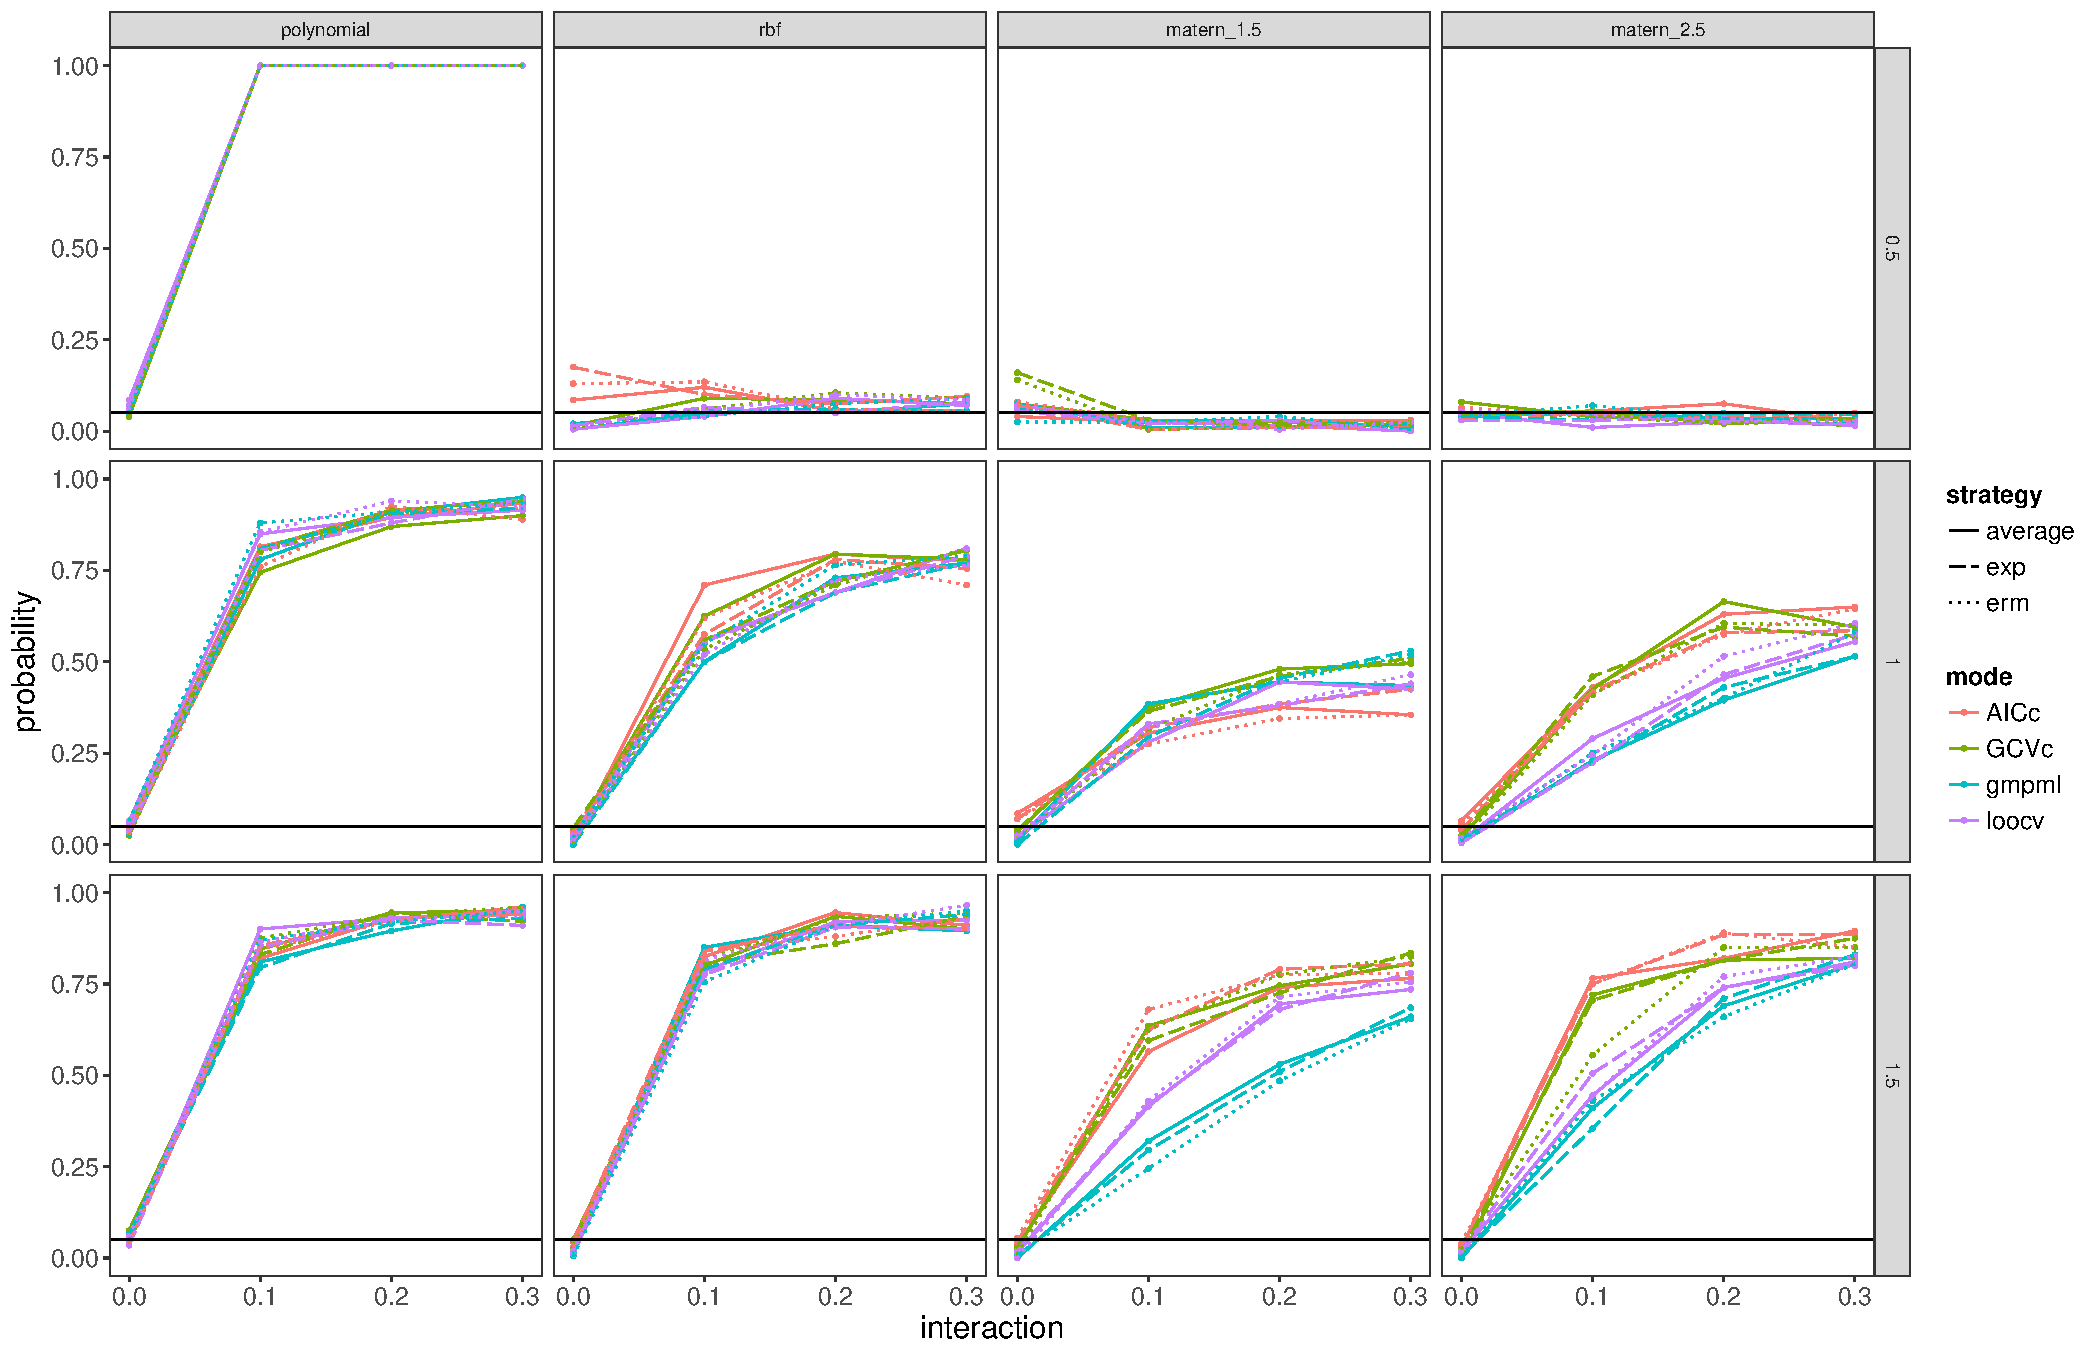
\includegraphics[width=0.9\columnwidth]{A1} 
\caption{Asym, True kernel only}
\label{fig:res}
\end{center}
\end{figure}

\begin{figure}
\begin{center}
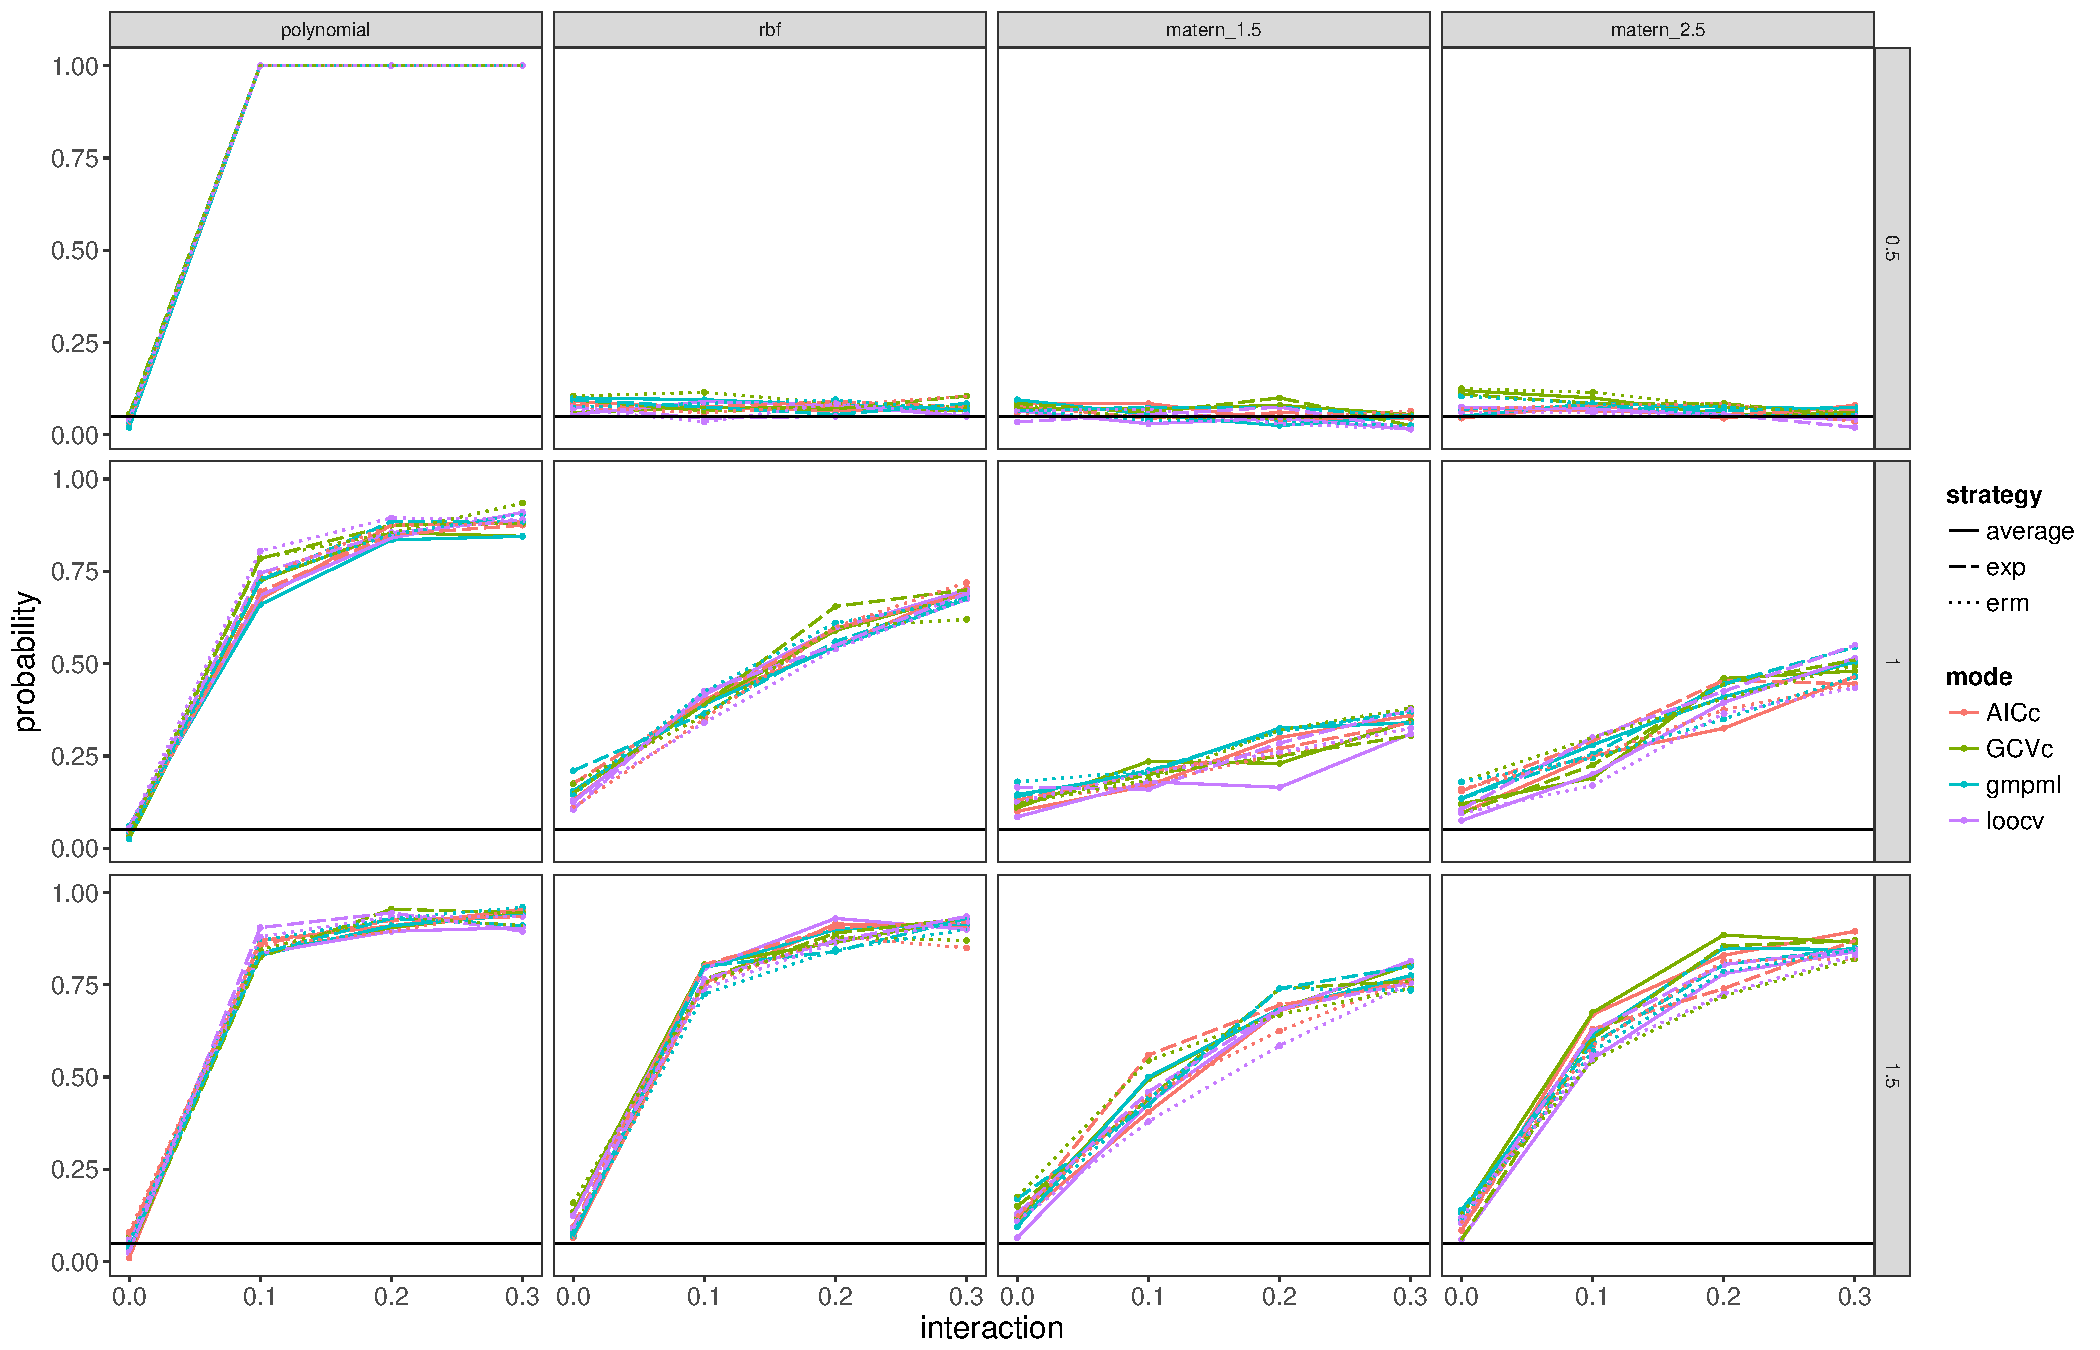
\includegraphics[width=0.9\columnwidth]{A2} 
\caption{Asym, 3 Polynomial kernels}
\label{fig:res}
\end{center}
\end{figure}

\begin{figure}
\begin{center}
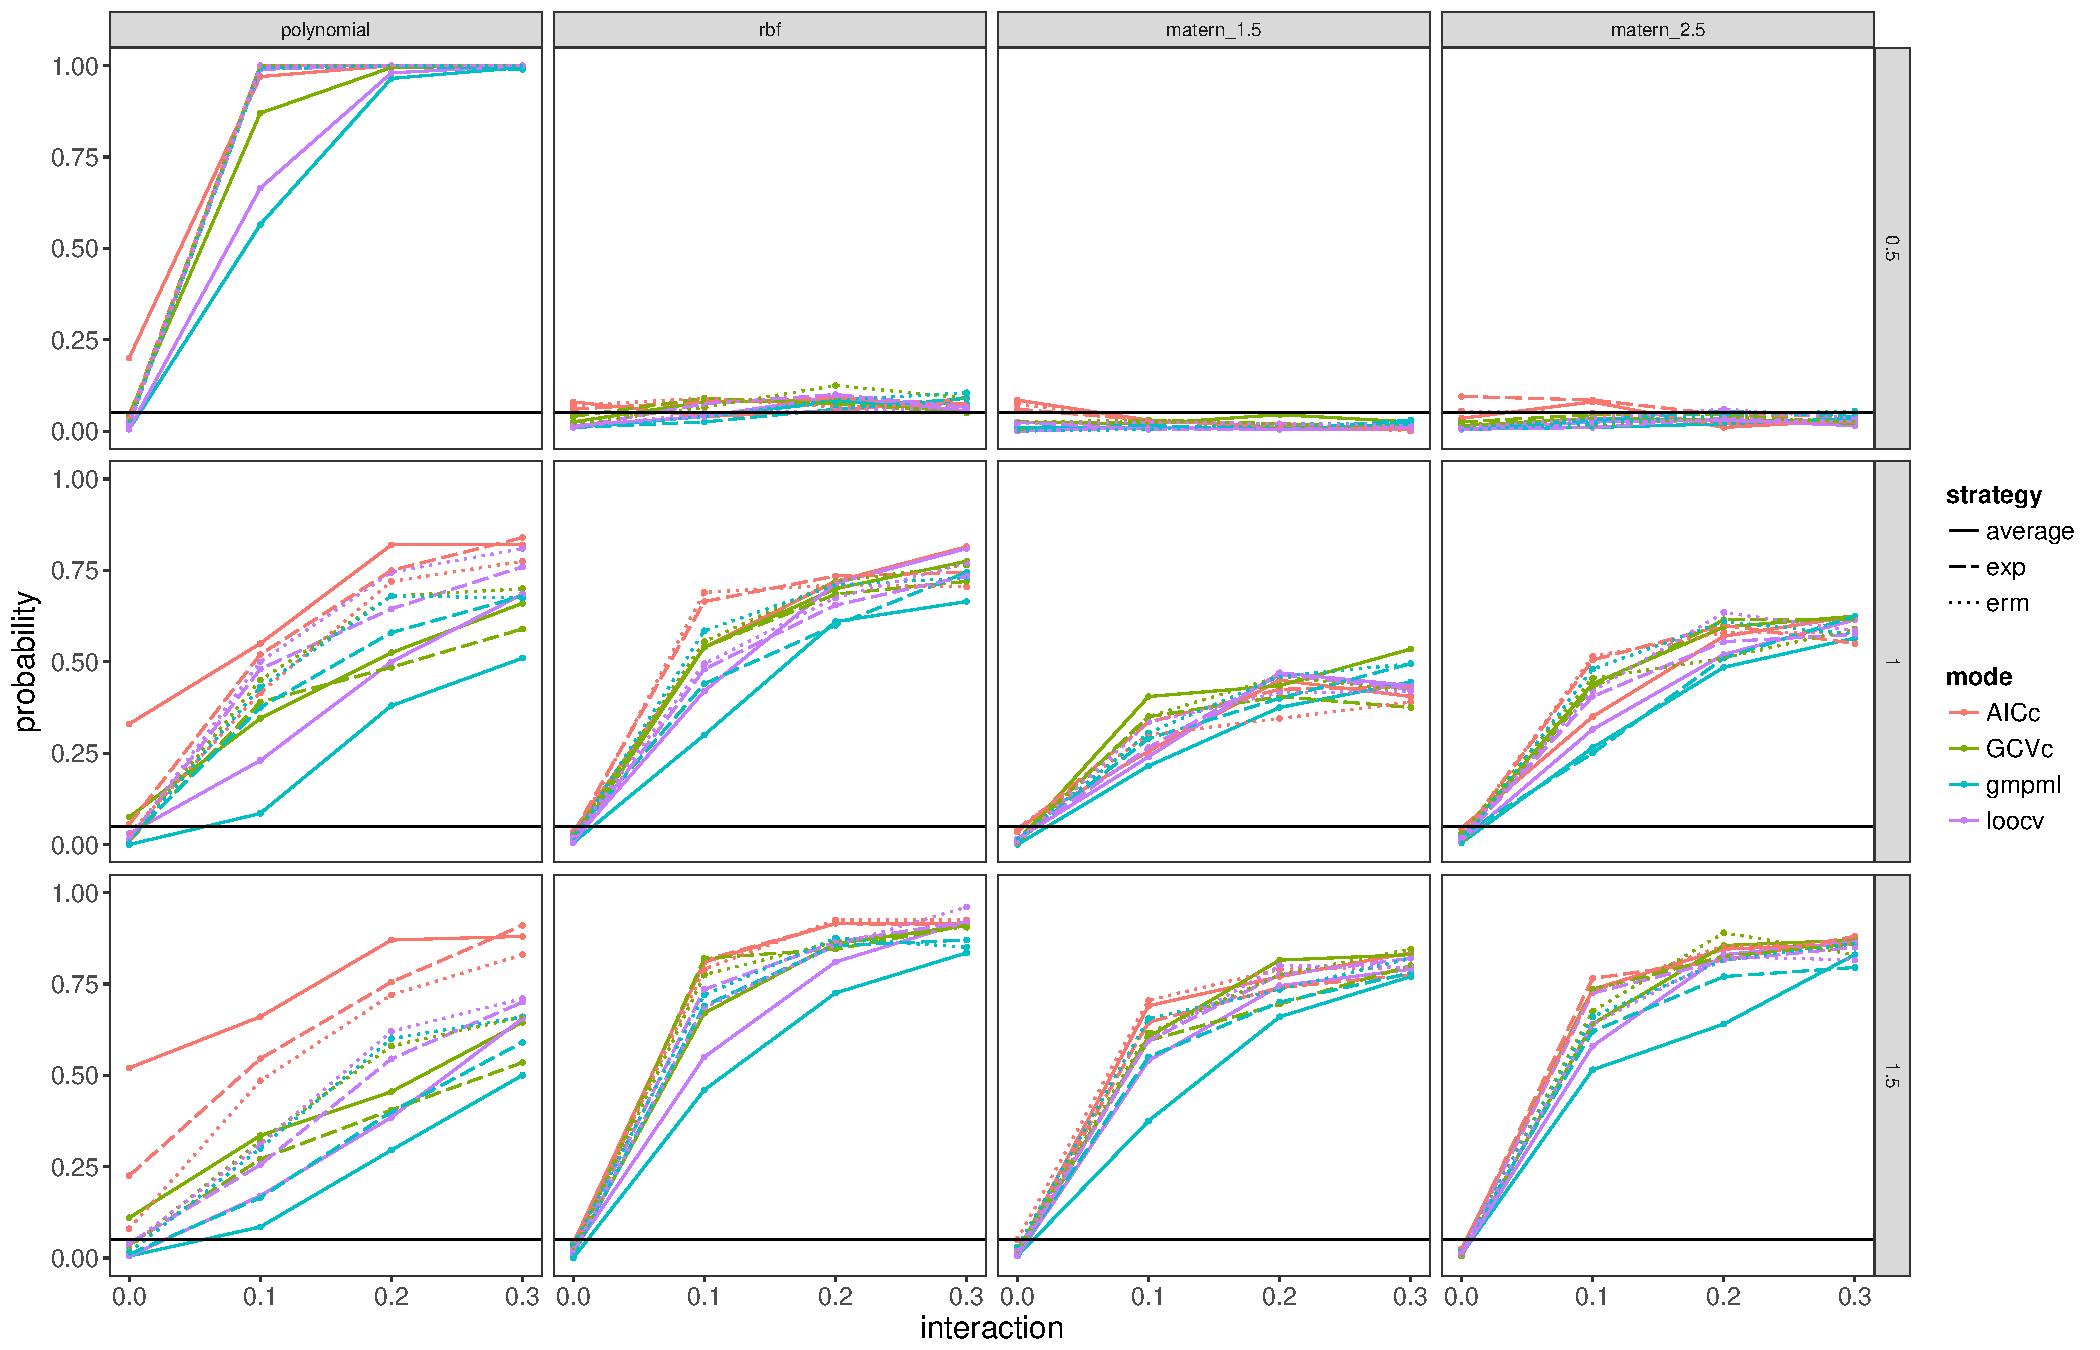
\includegraphics[width=0.9\columnwidth]{A3} 
\caption{Asym, 3 RBF kernels}
\label{fig:res}
\end{center}
\end{figure}

\begin{figure}
\begin{center}
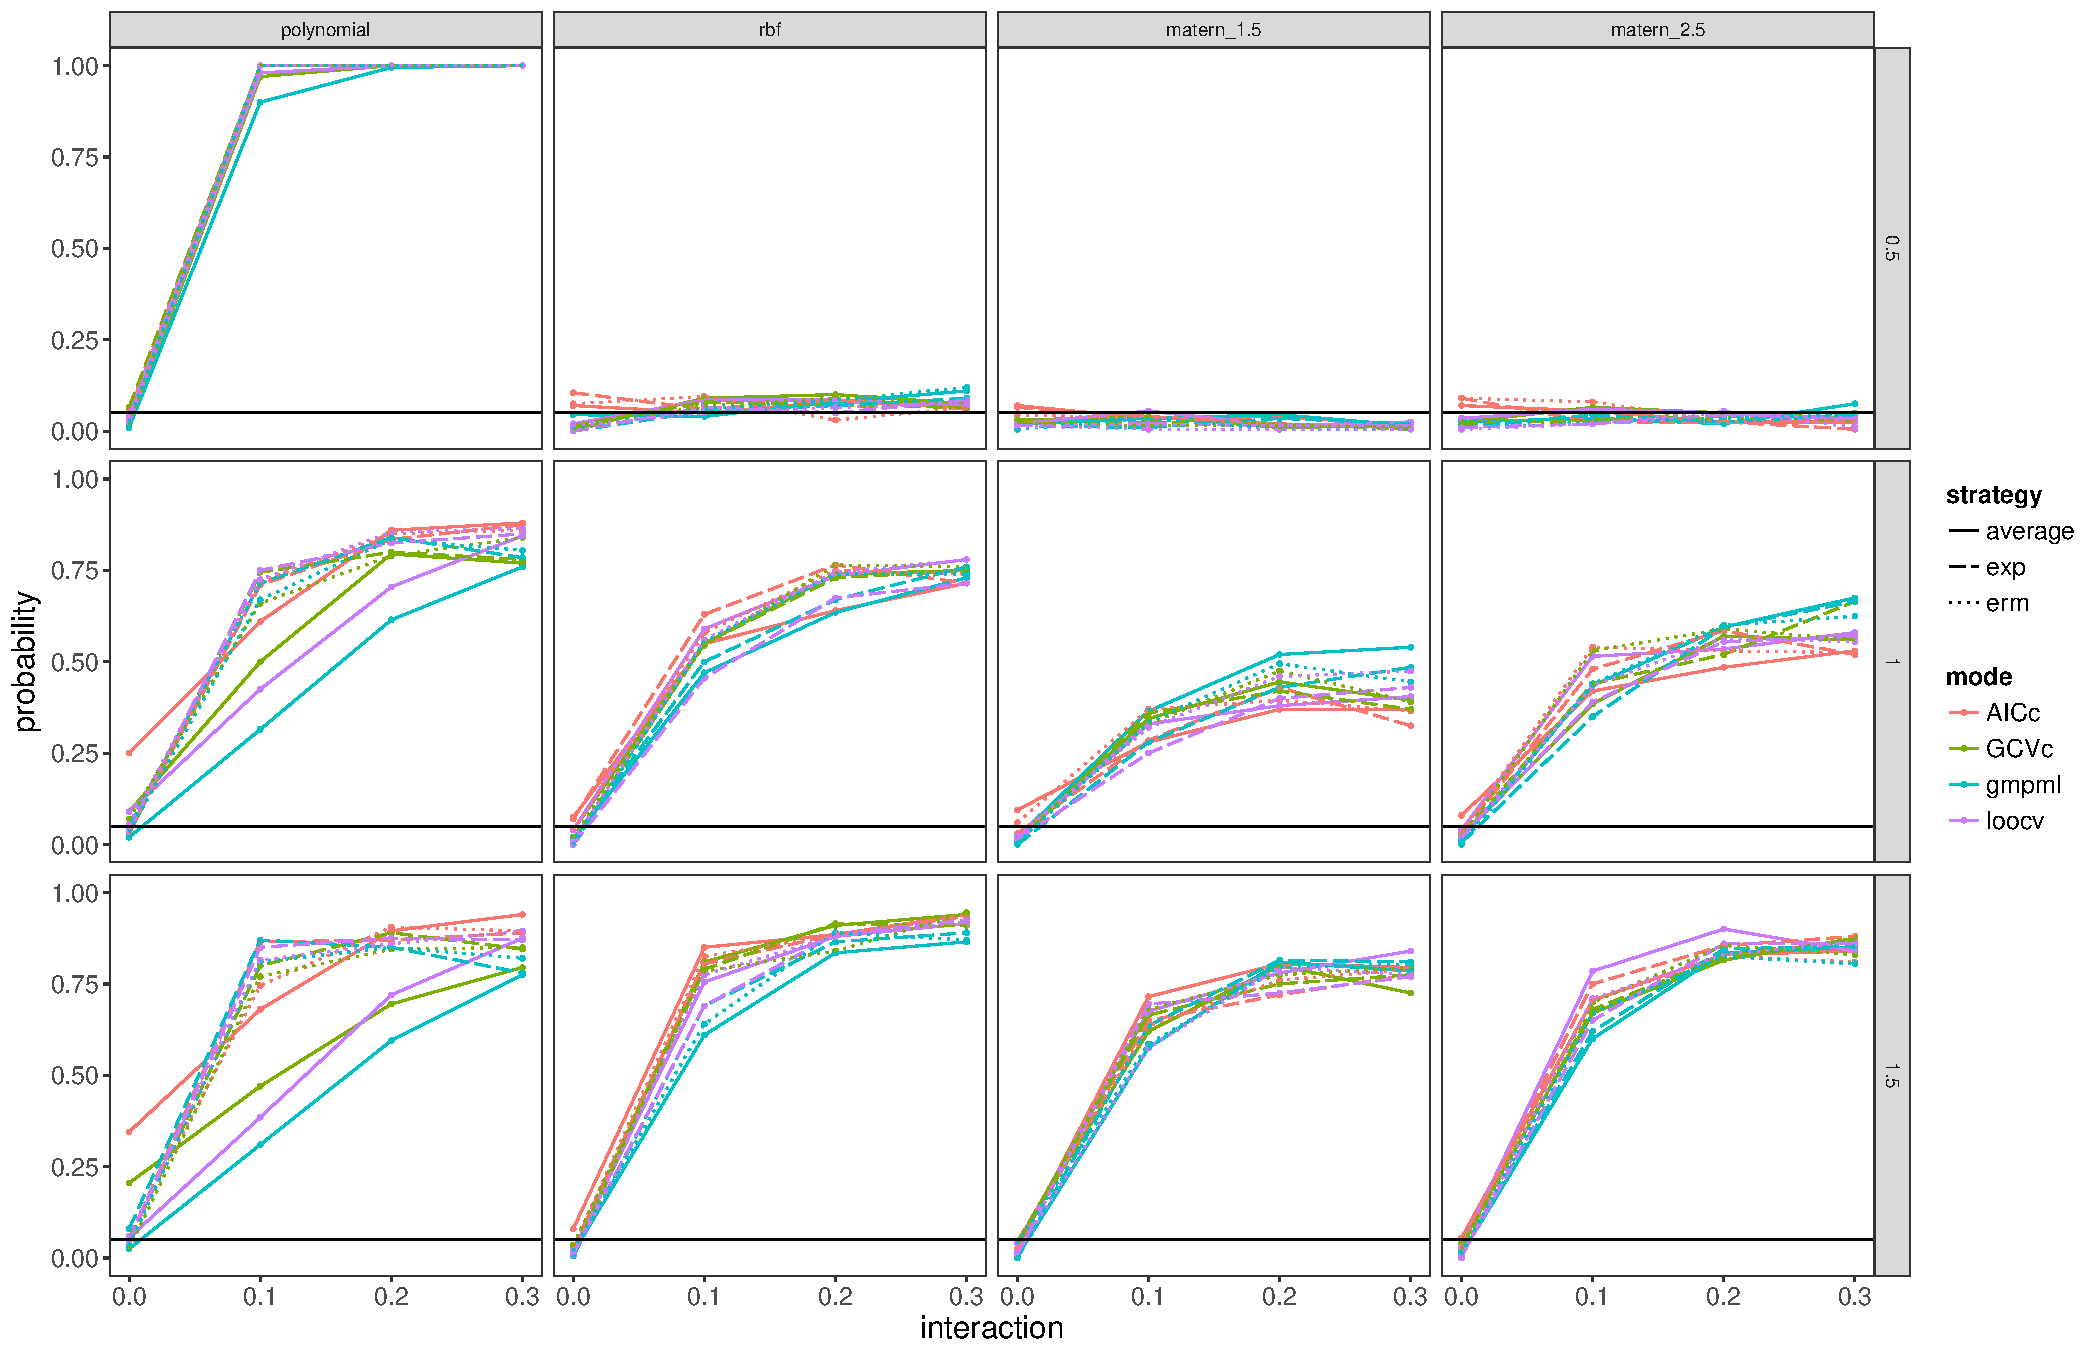
\includegraphics[width=0.9\columnwidth]{A4} 
\caption{Asym, 3 Polynomial kernels and 3 RBF kernels}
\label{fig:res}
\end{center}
\end{figure}

\begin{figure}
\begin{center}
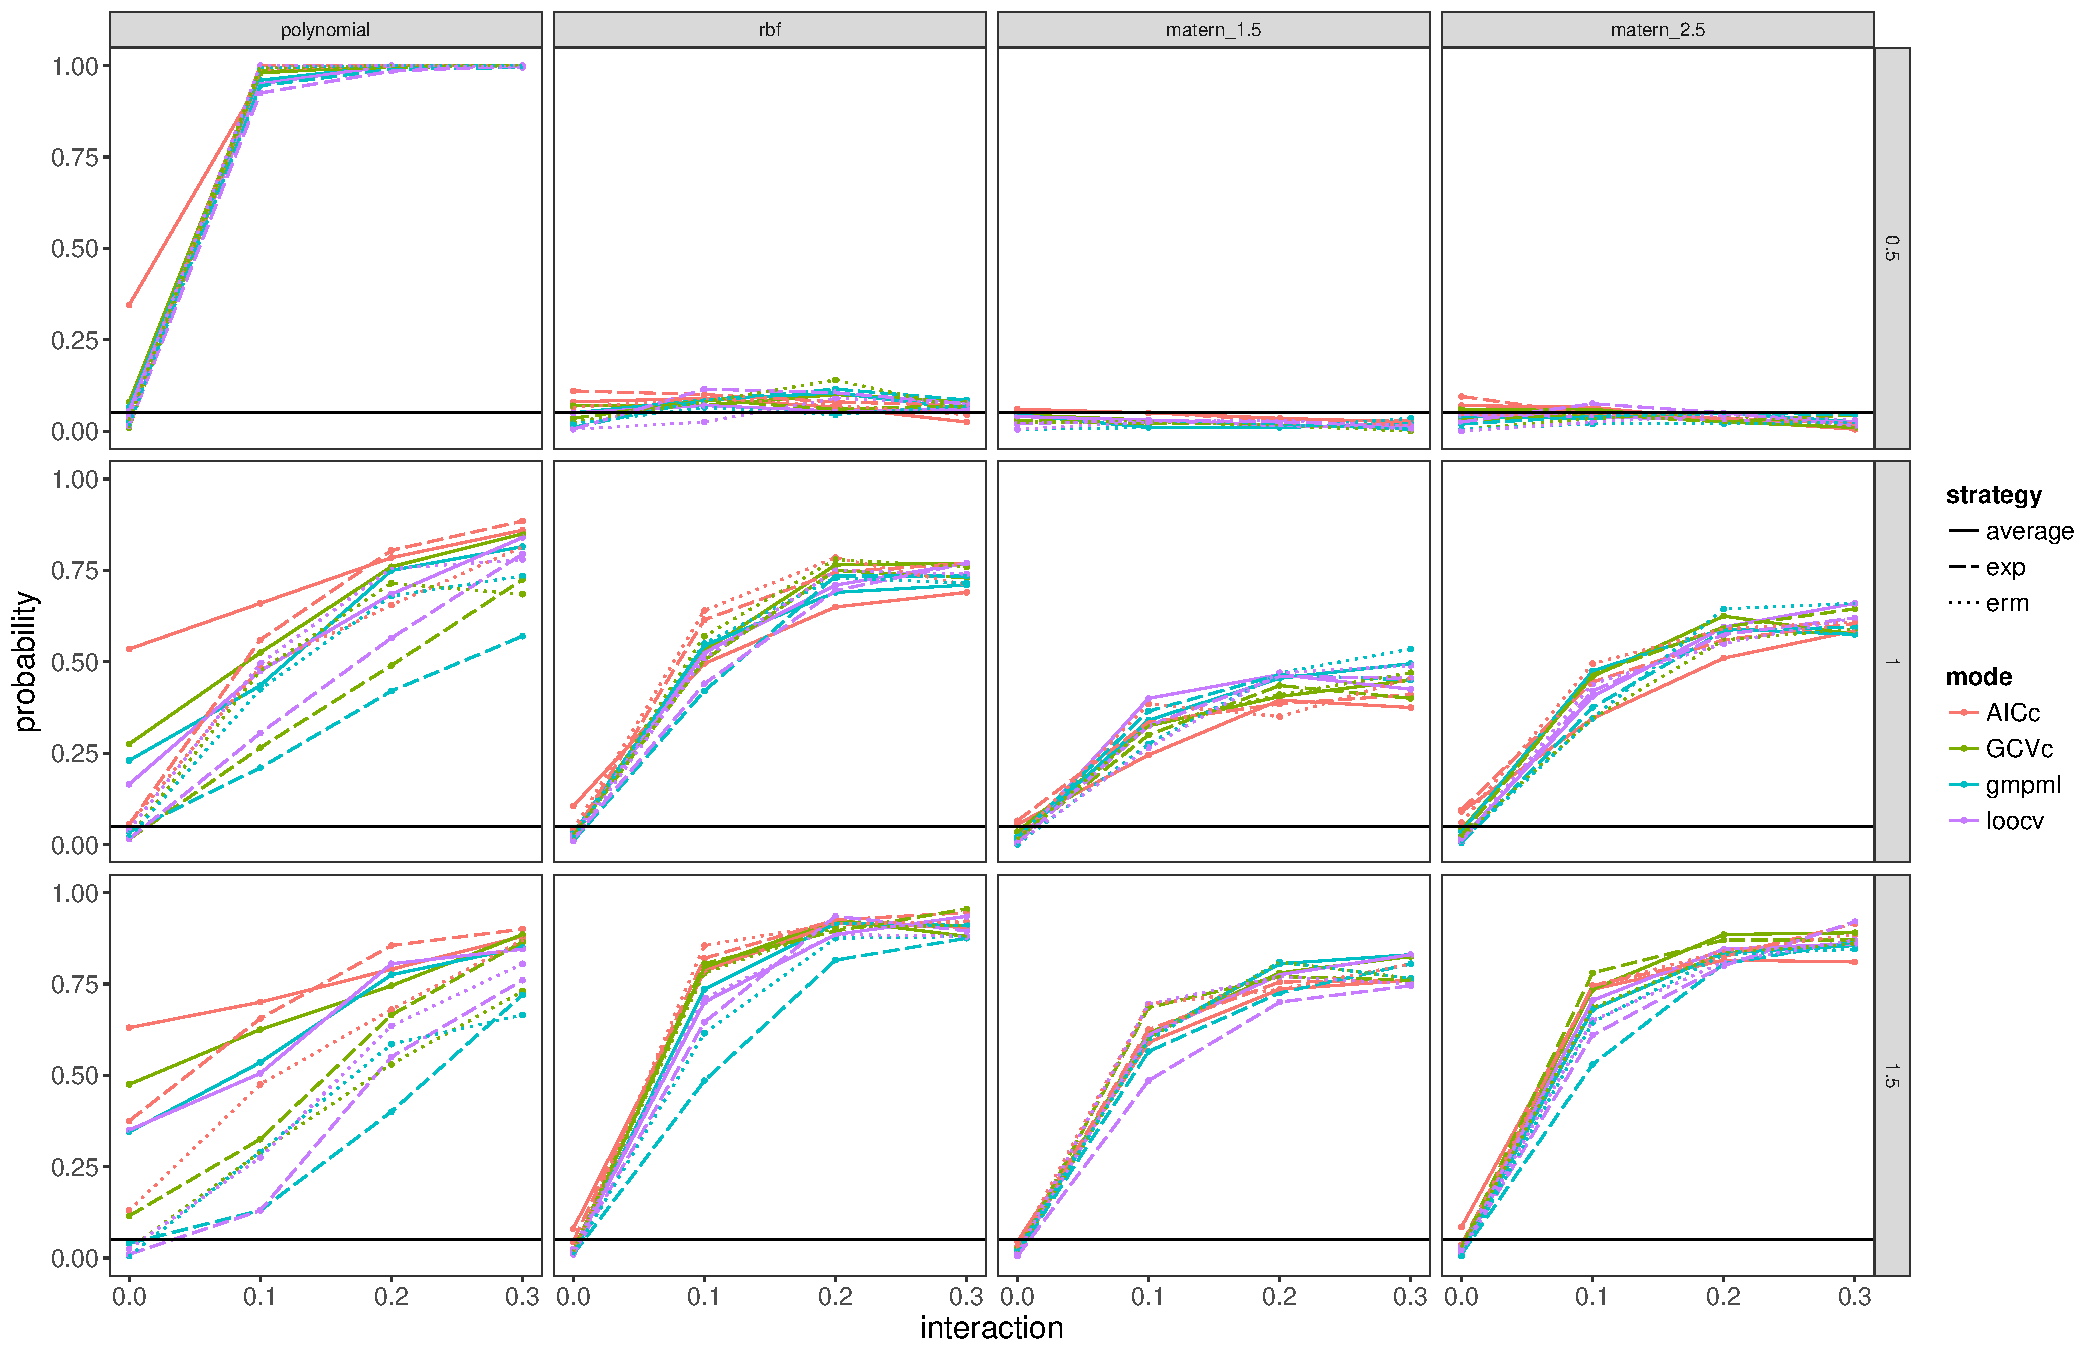
\includegraphics[width=0.9\columnwidth]{A5} 
\caption{Asym, 3 Matern kernels and 3 RBF kernels}
\label{fig:res}
\end{center}
\end{figure}

\begin{figure}
\begin{center}
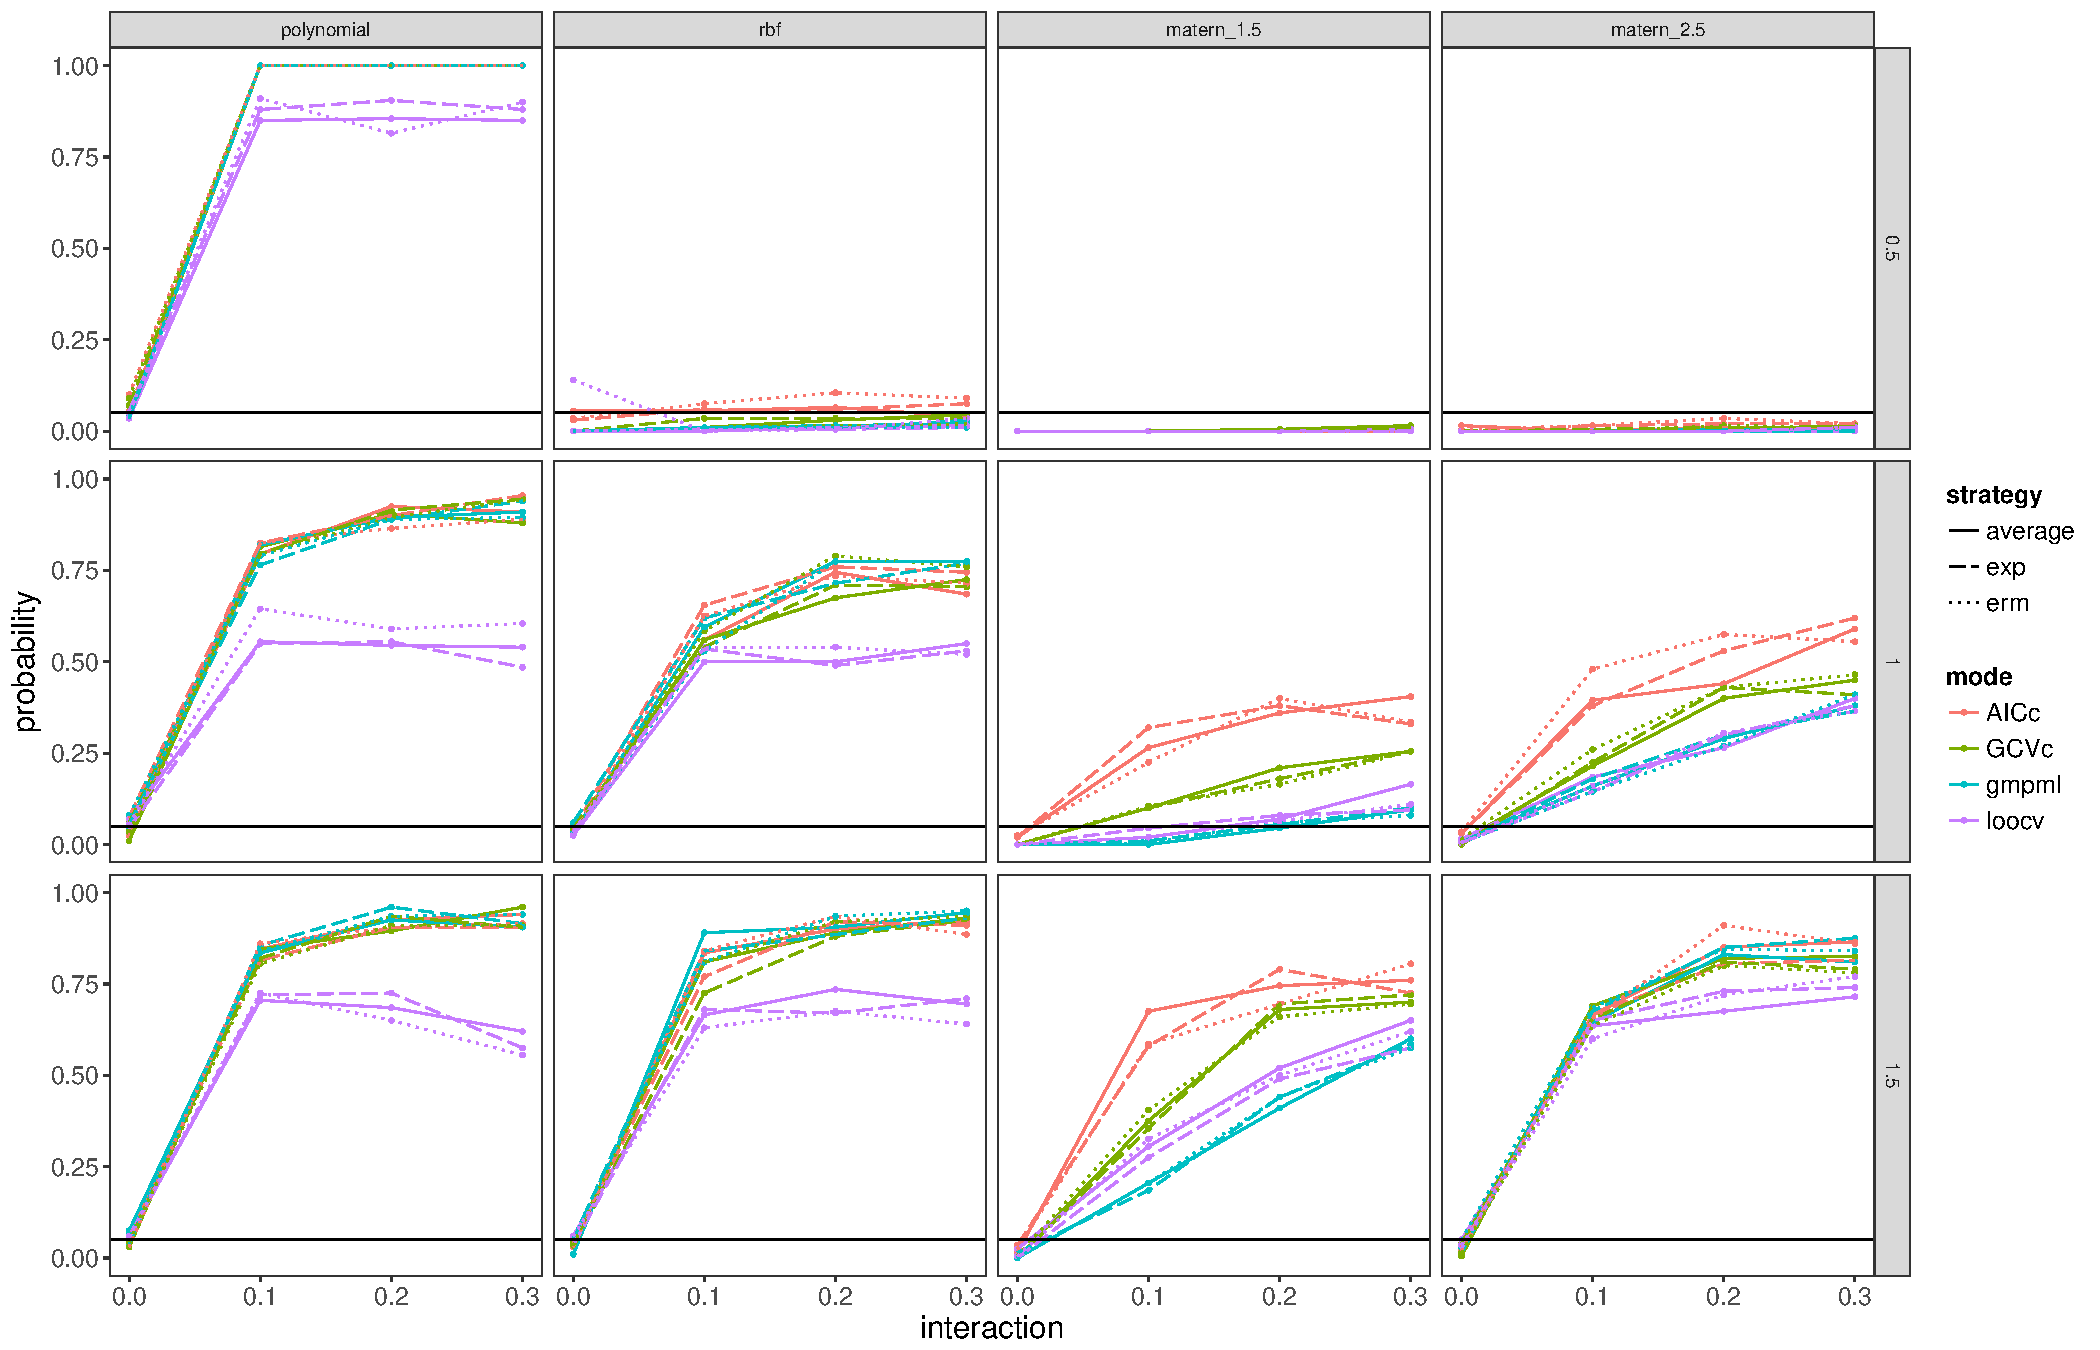
\includegraphics[width=0.9\columnwidth]{B1} 
\caption{Boot, True kernel only}
\label{fig:res}
\end{center}
\end{figure}

\begin{figure}
\begin{center}
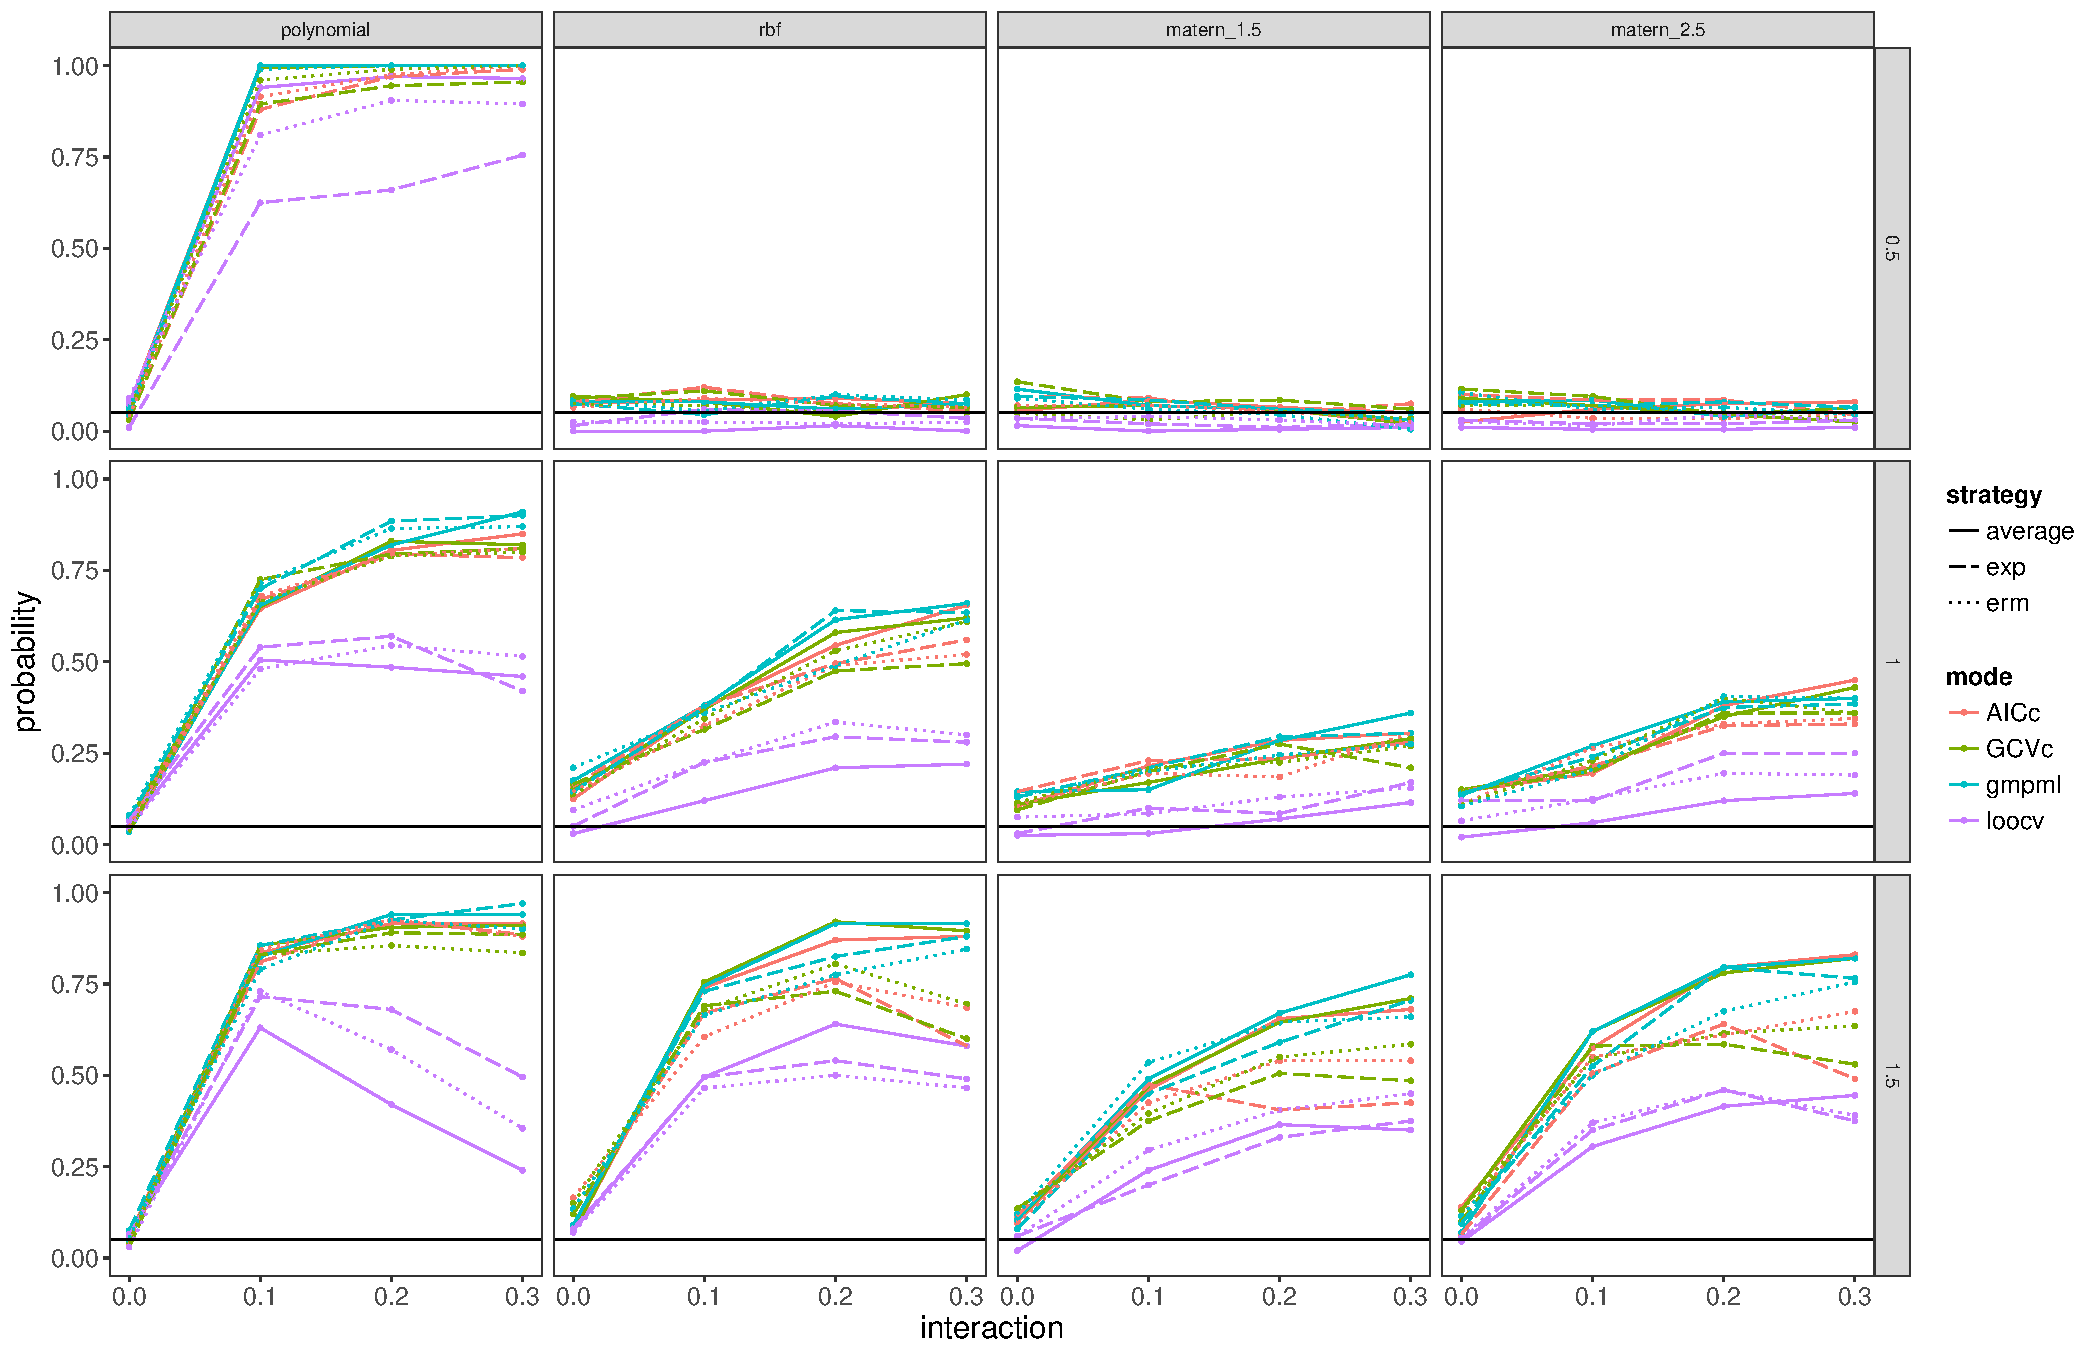
\includegraphics[width=0.9\columnwidth]{B2} 
\caption{Boot, 3 Polynomial kernels}
\label{fig:res}
\end{center}
\end{figure}

\begin{figure}
\begin{center}
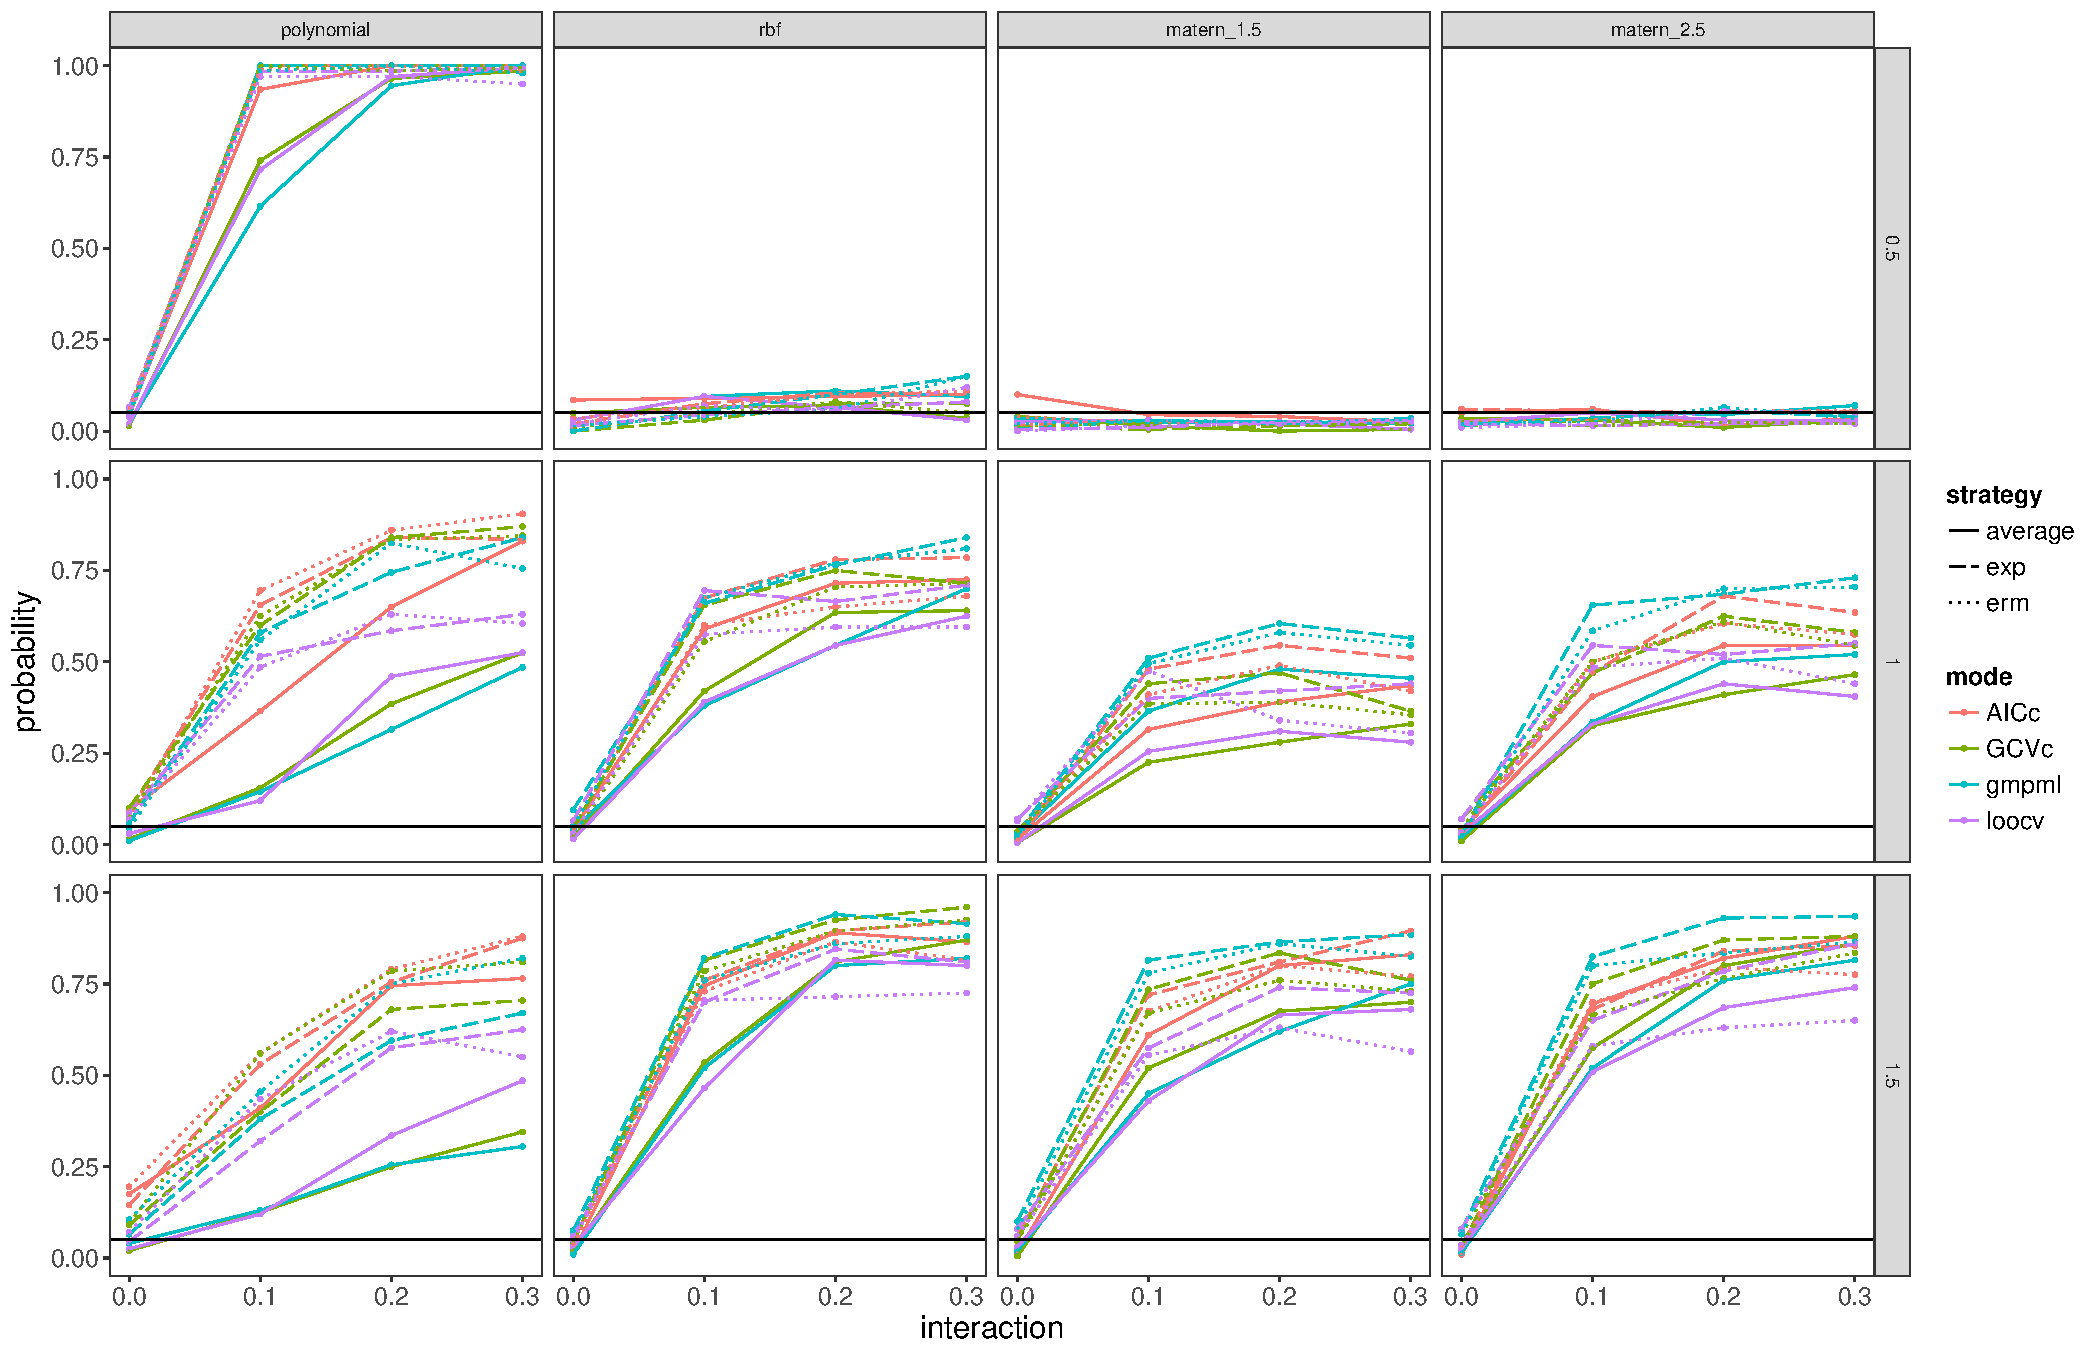
\includegraphics[width=0.9\columnwidth]{B3} 
\caption{Boot, 3 RBF kernels}
\label{fig:res}
\end{center}
\end{figure}

\begin{figure}
\begin{center}
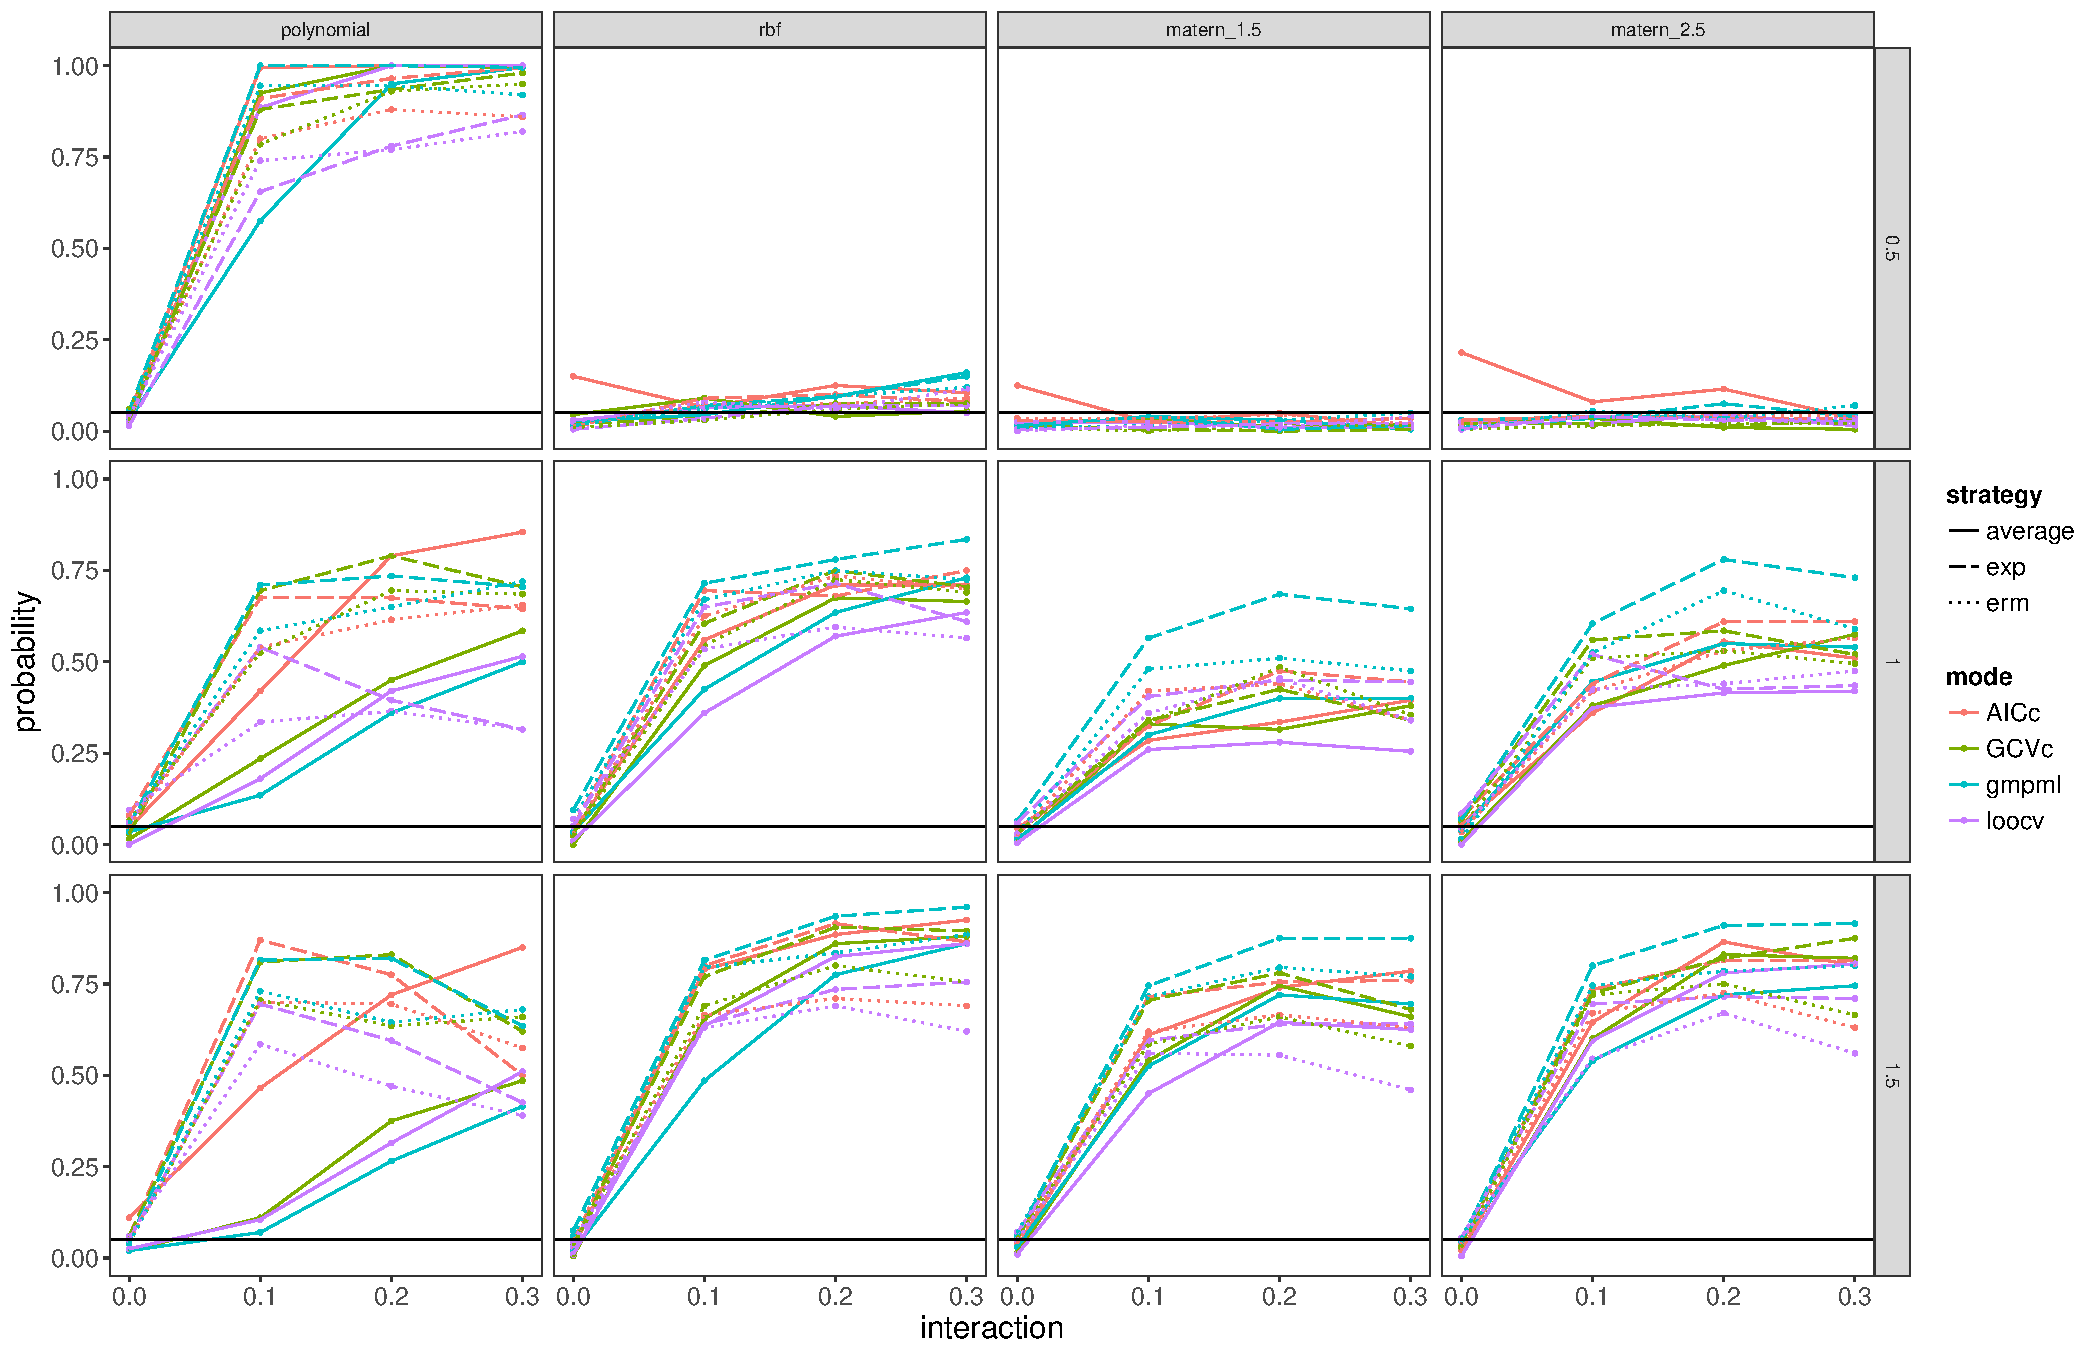
\includegraphics[width=0.9\columnwidth]{B4} 
\caption{Boot, 3 Polynomial kernels and 3 RBF kernels}
\label{fig:res}
\end{center}
\end{figure}

\begin{figure}
\begin{center}
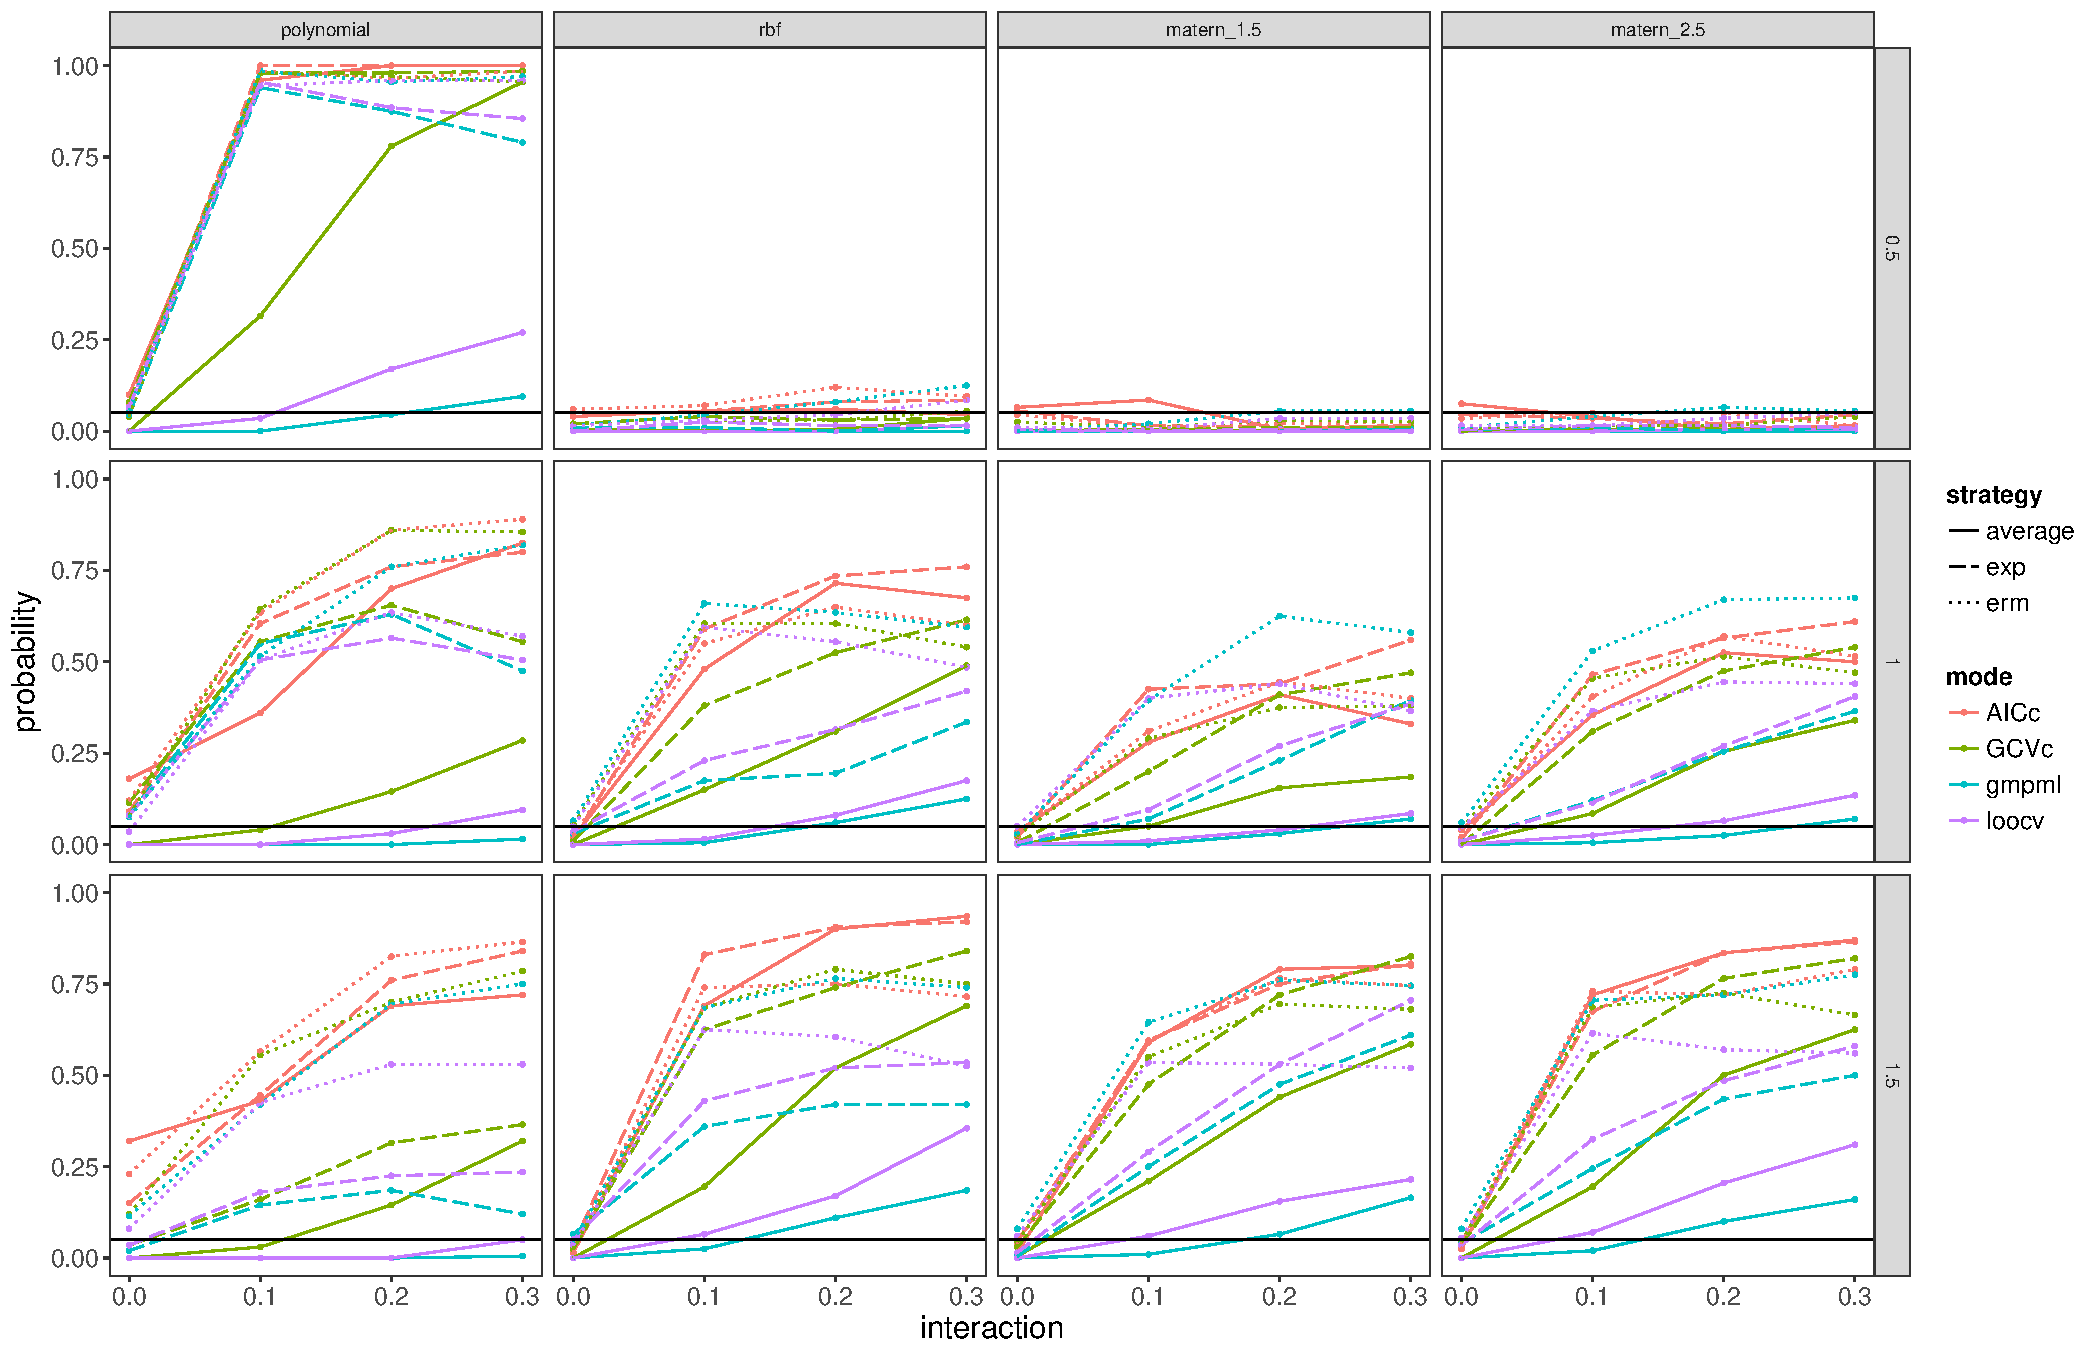
\includegraphics[width=0.9\columnwidth]{B5} 
\caption{Boot, 3 Matern kernels and 3 RBF kernels}
\label{fig:res}
\end{center}
\end{figure}

\section*{Acknowledgments}
The authors are grateful to the Department of Biostatistics at the Harvard Chan School, with special thanks to Dr. Erin Lake for offering insightful instructions and helpful resources.

\clearpage


%% -- Bibliography -------------------------------------------------------------
%% - References need to be provided in a .bib BibTeX database.
%% - All references should be made with \cite, \citet, \citep, \citealp etc.
%%   (and never hard-coded). See the FAQ for details.
%% - JSS-specific markup (\proglang, \pkg, \code) should be used in the .bib.
%% - Titles in the .bib should be in title case.
%% - DOIs should be included where available.

\bibliography{refs}


%% -- Appendix (if any) --------------------------------------------------------
%% - After the bibliography with page break.
%% - With proper section titles and _not_ just "Appendix".

\newpage

\begin{appendix}
\setcounter{equation}{0}
\renewcommand{\theequation}{App.\arabic{equation}}
\section{Derivation of Derivative wrt lambda} \label{app:technical}

Corresponding to (2.2.3),
\begin{align*}
\by=\bmu+\bh+\bepsilon \quad \mbox{where} \quad \bh \sim \mathrm{N}(\mathbf{0}, \tau \bK_\delta) \quad \bepsilon \sim \mathrm{N}(\mathbf{0}, \sigma^2\bI),
\end{align*}
where $\bK_\delta$ is the kernel matrix generated by $k_{\delta}(\bz, \bz')$.

The general model may be expressed in matrix form as \citep{reiss_smoothing_2009}:
\begin{align}
\by=\bmu+\Phi(\bX)^\top  \bbeta+\bepsilon \quad \mbox{where}\; \Phi(\bX)^\top \;\mbox{is}\; n\times p, \label{bb}
\end{align}
where $\Phi(\bX)$ is the aggregation of columns $\phi(\bx)$ for all cases in the training set, and $\phi(\bx)$ is a function mapping a $D$-dimensional input vector $\bx$ into an $p$-dimensional feature space. This model is fitted by penalized least squares, i.e., our estimate is
\begin{align}
(\hat{\mu}, \hat{\bbeta})=\underset{\mu, \bbeta}{\mbox{argmin}} \; (\parallel \by-\bmu-\Phi(\bX)^\top \bbeta \parallel^2+\lambda \bbeta^\top \bbeta). \label{cc}
\end{align}
The development that follows depends on the following Assumptions:
\begin{itemize}
\item $\bf{1}^\top \Phi(\bX)^\top=\mathbf{0}$,
\item $\by$ is not in the column space of $\bf{1}$,
\end{itemize}
where $\mathbf{1}$ is a $n\times 1$ vector.

\subsection{Derivative of REML}

As our choice of matrix notation suggests, model \eqref{bb} can be seen as equivalent to a linear mixed model, in the following sense. The criterion in \eqref{cc} is proportional to the log likelihood for the partly observed ``data'' $(\by, \bbeta)$ with respect to the unknowns $\bmu$ and $\bbeta$, i.e., the best linear unbiased prediction (BLUP) criterion, for the mixed model
\begin{align*}
\by|\bbeta \sim \mathrm{N}(\bmu+\Phi(\bX)^\top \bbeta, \sigma^2\bI), \quad \bbeta \sim \mathrm{N}(0, (\sigma^2/\lambda) \bI).
\end{align*}

Under this model, $Var(\by)=\sigma^2 \bV_\lambda$ where
\begin{align}
\bV_\lambda=\bI+\lambda^{-1}\Phi(\bX)^\top \Phi(\bX)=\bI+\lambda^{-1}\bK_\delta.
\end{align}

The mixed model formulation motivates treating $\lambda$ as a variance parameter to be estimated by maximizing the log likelihood
\begin{align*}
l(\mu, \lambda, \sigma^2|\by)=-\frac{1}{2}\Big[\mbox{log}| \sigma^2 \bV_\lambda | +(\by-\bmu)^\top (\sigma^2 \bV_\lambda)^{-1}(\by-\bmu) \Big]
\end{align*}
Maximizing this log likelihood results in estimating $\sigma^2$ with a downward bias, which is removed if we instead maximize the restricted log likelihood
\begin{align}
l_R(\mu, \lambda, \sigma^2|\by)=-\frac{1}{2}\Big[\mbox{log}| \sigma^2 \bV_\lambda | +(\by-\bmu)^\top (\sigma^2 \bV_\lambda)^{-1}(\by-\bmu)+\mbox{log} | \sigma^{-2}\mathbf{1}^\top \bV_\lambda^{-1}\mathbf{1} | \Big]. \label{aa} 
\end{align}

We shall refer to the resulting estimate of $\lambda$ as the REML choice of the parameter.\\
For given $\mu$ and $\lambda$, the value of $\sigma^2$ maximizing the restricted log likelihood \eqref{aa} is
\begin{align}
\hat{\sigma}_{\mu, \lambda}^2=(\by-\bmu)^\top \bV_\lambda^{-1}(\by-\bmu)/(n-1).
\end{align}

Substituting in this value and ignoring an additive constant leads to the profile restricted log likelihood
\begin{align}
l_R(\mu, \lambda|\by)=-\frac{1}{2}\Big[\mbox{log}| \bV_\lambda | +\mbox{log} | \mathbf{1}^\top \bV_\lambda^{-1}\mathbf{1} |+(n-1)\mbox{log}\{(\by-\bmu)^\top  \bV_\lambda^{-1}(\by-\bmu)\}\Big]. \label{ee}
\end{align}

For given $\lambda$, the value of $\mu$ maximizing this last expression is the generalized least square fit $\hat{\mu}_\lambda=(\mathbf{1}^\top \bV_\lambda^{-1}\mathbf{1})^{-1}\mathbf{1}^\top \bV_\lambda^{-1}\by$.

Using the readily verified equality $\bV_\lambda^{-1}=\bI-\bA_\lambda$, the following key facts about $\bP_\lambda$ can be shown to hold under Assumptions 1-2:
\begin{align}
\bP_\lambda=\bI-\bH_\lambda, \label{mm}
\end{align}
where $\bH_\lambda$ is the hat matrix defined by $\hat{\by}=\bH_\lambda \by$ and given by
\begin{align}
\bH_\lambda=\mathbf{1}(\mathbf{1}^\top \mathbf{1})^{-1}\mathbf{1}^\top &+\bA_\lambda,\\
\bV_\lambda^{-1}\mathbf{1}=\mathbf{1} \label{dd}, \\
\bP_\lambda^k=\bV_\lambda^{-k}-\mathbf{1}(\mathbf{1}^\top \mathbf{1})^{-1}&\mathbf{1}^\top. \;\mbox{for}\;k=1,\;2,...\label{ii}
\end{align}

Under Assumptions 1-2, repeated application of \eqref{dd} gives $\by-\hat{\bmu}_\lambda=[\bI-\mathbf{1}(\mathbf{1}^\top \mathbf{1})^{-1}\mathbf{1}^\top ]\by$, and hence
\begin{align}
(\by-\hat{\bmu}_\lambda)^\top \bV_\lambda^{-1}(\by-\hat{\bmu}_\lambda)=\by^\top \bP_\lambda \by.\label{ff}
\end{align}

Substituting \eqref{ff} into \eqref{ee} yields the profile restricted log likelihood for $\lambda$ alone:
\begin{align}
l_R(\lambda|\by)=-\frac{1}{2}\Big[\mbox{log}| \bV_\lambda | +\mbox{log} | \mathbf{1}^\top \bV_\lambda^{-1}\mathbf{1} |+(n-1)\mbox{log}(\by^\top \bP_\lambda \by)\Big] \label{gg}
\end{align}

Setting the derivative of \eqref{gg} with respect of $\lambda$ to zero will yield an equation for the REML estimate of $\lambda$. By \eqref{dd} again, $\mbox{log} | \mathbf{1}^\top \bV_\lambda^{-1}\mathbf{1} |=\mbox{log} | \mathbf{1}^\top \mathbf{1} |$, which does not depend on $\lambda$, so the differentiation reduces to finding the derivatives of $\mbox{log}| \bV_\lambda |$ and $\mbox{log}(\by^\top \bP_\lambda \by)$. To that end we shall need the (component-wise) derivatives of $\bV_\lambda$ and $\bP_\lambda$ with respect to $\lambda$. These can be shown to be:
\begin{align}
\frac{\partial \bV_\lambda}{\partial \lambda}=&\lambda^{-1}(\bI-\bV_\lambda), \label{hh} \\
\frac{\partial \bP_\lambda}{\partial \lambda}=&\lambda^{-1}(\bP_\lambda-\bP_\lambda^2). \label{jj}
\end{align}

A formula in \citep{lindstrom_newtonraphson_1988}(p. 1016), together with \eqref{hh}, leads to
\begin{align*}
\frac{\partial}{\partial \lambda}\mbox{log}| \bV_\lambda |=\lambda^{-1}\mbox{tr}(\bV_\lambda^{-1}-\bI).
\end{align*}

By \eqref{ii}, $\mbox{tr}(\bV_\lambda^{-1})=\mbox{tr}(\bP_\lambda)+\mbox{tr}[\bI-\mathbf{1}(\mathbf{1}^\top \mathbf{1})^{-1}\mathbf{1}^\top ]=\mbox{tr}(\bP_\lambda)+1$, so we conclude that
\begin{align}
\frac{\partial}{\partial \lambda}\mbox{log}| \bV_\lambda |=\lambda^{-1}[\mbox{tr}(\bP_\lambda)-(n-1)]. \label{kk}
\end{align}

By Assumption 2, $\by^\top \bP_\lambda \by>0$. Thus, using \eqref{jj}, we obtain
\begin{align}
\frac{\partial}{\partial \lambda}\mbox{log}(\by^\top \bP_\lambda \by)=\lambda^{-1}\Big[1-\frac{\by^\top \bP_\lambda^2\by}{\by^\top \bP_\lambda \by} \Big]. \label{ll}
\end{align}

Under our Assumptions, the matrix
\begin{align*}
\bP_\lambda=\bV_\lambda^{-1}-\bV_\lambda^{-1}\mathbf{1}(\mathbf{1}^\top \bV_\lambda^{-1}\mathbf{1})^{-1}\mathbf{1}^\top \bV_\lambda^{-1}
\end{align*}
which plays a role in some treatments of mixed model theory, turns out to be important for both the REML and the GCV approach to choosing $\lambda$.

By \eqref{gg}, \eqref{kk} and \eqref{ll}, we obtain
\begin{align}
\frac{\partial l_R(\lambda|\by)}{\partial \lambda}=\frac{1}{2\lambda}\Big[(n-1)\frac{\by^\top \bP_\lambda^2\by}{\by^\top \bP_\lambda \by}- \mbox{tr}(\bP_\lambda)\Big]. \label{nn}
\end{align}

Thus by \eqref{mm}, \eqref{ff} and \eqref{nn}, $\frac{\partial l_R(\lambda|\by)}{\partial \lambda}=0$ implies
\begin{align}
\frac{(\by-\hat{\bmu}_\lambda)^\top \bV_\lambda^{-1}(\by-\hat{\bmu}_\lambda)}{n-1}=\frac{\by^\top  (\bI-\bH_\lambda)^2\by}{\mbox{tr}(\bI-\bH_\lambda)}. \label{oo}
\end{align}
which is also
\begin{align}
\frac{\by^\top \bP_\lambda \by}{n-1}=\frac{\by^\top  \bP_\lambda^2\by}{\mbox{tr}(\bP_\lambda)} \quad \mbox{or} \quad \frac{\by^\top \bP_\lambda \by}{\by^\top  \bP_\lambda^2\by}=\frac{n-1}{\mbox{tr}(\bP_\lambda)},
\end{align}
where $\hat{\mu}_\lambda$ and $\bH_\lambda$ are the parameter estimate and hat matrix, respectively, obtained with smoothing parameter value $\lambda$. The left side of \eqref{oo} is the REML estimate of $\sigma^2$ \citep{wahba_spline_1990}. The right side equals $\parallel \by-\hat{\by}\parallel ^2/[n-\mbox{tr}(\bH_\lambda)]$, an estimate of $\sigma^2$ based on viewing $tr(\bH_\lambda)$ as the degrees of freedom of the smoother \citep{pawitan_all_2001}(p. 487) and \citep{lee_generalized_2006}(p. 279). In other words, when $\lambda$ is estimated by REML, the REML error variance estimate agrees with the ``smoothing-theoretic'' variance estimate.

\subsection{Derivative of GCV}
The GCV criterion is given by
\begin{align*}
GCV(\lambda)=\frac{\parallel \by-\hat{\by}\parallel ^2}{[1-\mbox{tr}(\bH_\lambda)/n]^2}=\frac{\by^\top  (\bI-\bH_\lambda)^2\by}{[\mbox{tr}(\bI-\bH_\lambda)]^2}=\frac{\by^\top  \bP_\lambda^2\by}{[\mbox{tr}(\bP_\lambda)]^2},
\end{align*}
with the last equality following from \eqref{mm}. This criterion, originally proposed by \citep{craven_smoothing_1979}, is an approximation to $\frac{1}{n}\sum_{i=1}^n \frac{(y_i-\hat{y}_i)^2}{(1-h_{\lambda [ii]})^2}$, where $h_{\lambda [11]},...,h_{\lambda [nn]}$ are the diagonal elements of $\bH_\lambda$. The latter expression can be shown (at least in some smoothing problems) to be equal to the leave-one-out cross-validation criterion, but lacks an invariance-under-reparametrization property that is gained by instead using GCV \citep{wahba_spline_1990}(pp. 52-53). Using \eqref{jj}, we can obtain
\begin{align}
\frac{\partial GCV(\lambda)}{\partial \lambda}=\frac{2}{\lambda [\mbox{tr}(\bP_\lambda)]^3}\Big[\mbox{tr}(\bP_\lambda^2)\by^\top  P_\lambda^2\by-\mbox{tr}(\bP_\lambda)\by^\top  P_\lambda^3\by \Big].
\end{align}

Thus at the GCV-minimizing $\lambda$ we have
\begin{align*}
\frac{\by^\top  \bP_\lambda^3\by}{\mbox{tr}(\bP_\lambda^2)}=\frac{\by^\top  \bP_\lambda^2\by}{\mbox{tr}(\bP_\lambda)}\quad \mbox{or} \quad \frac{\by^\top  \bP_\lambda^3\by}{\by^\top  \bP_\lambda^2\by}=\frac{\mbox{tr}(\bP_\lambda^2)}{\mbox{tr}(\bP_\lambda)}
\end{align*}

\subsection{Derivative of AIC}

The AIC criterion is given by
\begin{align*}
AIC(\lambda)=\mbox{log} (\parallel \by-\hat{\by}\parallel ^2)+\frac{2}{n}[\mbox{tr}(\bH_\lambda)+1]=\mbox{log}(\by^\top  \bP_\lambda^2\by)+\frac{2}{n}\mbox{tr}(\bI-\bP_\lambda)+\frac{2}{n}.
\end{align*}

Using \eqref{jj}, we can obtain
\begin{align}
\frac{\partial AIC(\lambda)}{\partial \lambda}=\frac{2}{\lambda}\Big[1-\frac{\by^\top  \bP_\lambda^3\by}{\by^\top  \bP_\lambda^2\by}-\frac{1}{n}\mbox{tr}(\bP_\lambda-\bP_\lambda^2)\Big].
\end{align}

Thus at the AIC-minimizing $\lambda$ we have
\begin{align*}
\frac{\by^\top  \bP_\lambda^3\by}{\by^\top  \bP_\lambda^2\by}=\frac{\mbox{tr}(\bI-\bP_\lambda+\bP_\lambda^2)}{n}.
\end{align*}


\section{Derivation of the REML based Test Statistic}
\subsection{Derivation of the Score Test Statistic}

In this section, we derive the score test statistic based on REML \citep{maity_powerful_2011}.\\ 
Denote $\bV(\btheta)=\sigma^2 \bV_\lambda=\sigma^2\bI+\tau \bK_\delta$, where $\btheta=(\delta, \tau, \sigma^2)$. The REML given in \eqref{aa} can be rewritten as
\begin{align}
l_R=-\frac{1}{2}\Big[\mbox{log}| \bV(\btheta) | +\mbox{log} | \mathbf{1}^\top \bV(\btheta)^{-1}\mathbf{1} | +(\by-\bmu)^\top \bV(\btheta)^{-1}(\by-\bmu)\Big]. \label{pp}
\end{align}

Under $H_0: \delta=0$ (2.2.2), we set $\btheta_0=(0, \tau, \sigma^2)$ and
\begin{align*}
\bP_0(\btheta_0)=\bV(\btheta_0)^{-1}-\bV(\btheta_0)^{-1}\mathbf{1}[\mathbf{1}^\top \bV(\btheta_0)^{-1}\mathbf{1}]^{-1}\mathbf{1}^\top \bV(\btheta_0)^{-1}.
\end{align*}

Take the derivative of \eqref{pp} with respect to $\delta$,
\begin{align}
\frac{\partial l_R}{\partial \delta}=&-\frac{1}{2}\Big[\frac{\partial \mbox{log}| \bV(\btheta) |}{\partial \delta}+\frac{\partial \mbox{log} | \mathbf{1}^\top \bV(\btheta)^{-1}\mathbf{1} |}{\partial \delta}+ \frac{\partial (\by-\bmu)^\top \bV(\btheta)^{-1}(\by-\bmu)}{\partial \delta}\Big]\nonumber \\
=&-\frac{1}{2}\Big[\mbox{tr}\big(\bV(\btheta)^{-1}\frac{\partial \bV(\btheta)}{\partial \delta}\big)+\mbox{tr}\big([\mathbf{1}^\top \bV(\btheta)^{-1}\mathbf{1}]^{-1}\mathbf{1}^\top \frac{\partial \bV(\btheta)^{-1}}{\partial \delta}\mathbf{1}\big)\nonumber \\
&+(\by-\bmu)^\top \frac{\partial \bV(\btheta)^{-1}}{\partial \delta}(\by-\bmu) \Big]\nonumber \\
=&-\frac{1}{2}\Big[\mbox{tr}\big(\bV(\btheta)^{-1}\tau (\partial \bK_\delta)\big)-\mbox{tr}\big(\tau (\partial \bK_\delta)\bV(\btheta)^{-1}\mathbf{1}[\mathbf{1}^\top \bV(\btheta)^{-1}\mathbf{1}]^{-1}\mathbf{1}^\top \bV(\btheta)^{-1}\big)\nonumber \\
&-(\by-\bmu)^\top \bV(\btheta)^{-1}\tau (\partial \bK_\delta)\bV(\btheta)^{-1}(\by-\bmu) \Big]\nonumber \\
=&\frac{1}{2}(\by-\bmu)^\top \bV(\btheta)^{-1}\tau (\partial \bK_\delta)\bV(\btheta)^{-1}(\by-\bmu)\nonumber \\
&-\frac{1}{2}\mbox{tr}\Big[\tau (\partial \bK_\delta)\big[\bV(\btheta)^{-1}-\bV(\btheta)^{-1}\mathbf{1}[\mathbf{1}^\top \bV(\btheta)^{-1}\mathbf{1} ]^{-1}\mathbf{1}^\top \bV(\btheta)^{-1}\big]\Big], \label{qq}
\end{align}
where $\partial \bK_\delta$ is the derivative kernel matrix whose $(i,j)^{th}$ entry is $\frac{\partial k_\delta(\bx, \bx')}{\partial \delta}$. If we further denote $\bK_0=\bK_\delta |_{\delta=0}$ and $\partial \bK_0=(\partial \bK_\delta)|_{\delta=0}$, we get the REML based score function of $\delta$ evaluated at $H_0$
\begin{align*}
S_{\delta=0}=\frac{1}{2}(\by-\bmu)^\top \bV(\btheta_0)^{-1}\tau (\partial \bK_0)\bV(\btheta_0)^{-1}(\by-\bmu)-\frac{1}{2}\mbox{tr}[\tau (\partial \bK_0)\bP_0].
\end{align*}

To test for $H_0: \delta=0$, we propose to use the score-based test statistic
\begin{align}
\hat{T}_0=\hat{\tau}(\by-\hat{\bmu})^\top \bV_0^{-1} (\partial \bK_0)\bV_0^{-1}(\by-\hat{\bmu}),
\end{align}
where $\bV_0=\hat{\sigma}^2\bI+\hat{\tau}\bK_0$.


\subsection{The Null Distribution of the Test Statistic}

For simplicity, we denote
\begin{align*}
\bV&=\bV(\btheta),\\
\bP=\bP(\btheta)=\bV^{-1}&-\bV^{-1}\mathbf{1}[\mathbf{1}^\top \bV^{-1}\mathbf{1}]^{-1}\mathbf{1}^\top \bV^{-1}.
\end{align*}

With similar derivation as \eqref{qq}, for each $\theta_i \in \btheta=(\delta, \tau, \sigma^2)$, we have
\begin{align}
\frac{\partial l_R}{\partial \theta_i}=-\frac{1}{2}\Big[\mbox{tr}\big(\bP \frac{\partial \bV}{\partial \theta_i}\big)-(\by-\bmu)^\top \bV^{-1}\big(\frac{\partial \bV}{\partial \theta_i}\big)\bV^{-1}(\by-\bmu)\Big]. \label{rr}
\end{align}

From \citep{liu_semiparametric_2007} we know $\hat{\bmu}=[\mathbf{1}^\top \bV^{-1}\mathbf{1}]^{-1}\mathbf{1}^\top \bV^{-1}\by$, plug it in \citep{lin_inference_1999}, we obtain 
\begin{align*}
(\by-\bmu)^\top \bV^{-1}=\by^\top  \big(\bI-\mathbf{1}[\mathbf{1}^\top \bV^{-1}\mathbf{1}]^{-1}\mathbf{1}^\top \bV^{-1}\big)^\top \bV^{-1}=\by^\top.  \bP
\end{align*}

\eqref{ss} becomes 
\begin{align*}
\frac{\partial l_R}{\partial \theta_i}=-\frac{1}{2}\Big[\mbox{tr}\big(\bP \frac{\partial \bV}{\partial \theta_i}\big)-\by^\top  \bP\big(\frac{\partial \bV}{\partial \theta_i}\big)\bP \by \Big].
\end{align*}

The second-order partial derivatives with respect to $\theta_i$ and $\theta_j$ is 
\begin{align}
\frac{\partial^2 l_R}{\partial \theta_i \partial \theta_j}=&-\frac{1}{2}\Big[\mbox{tr}\big(\frac{\partial \bP}{\partial \theta_j} \frac{\partial \bV}{\partial \theta_i}\big)+\mbox{tr}\big(\bP \frac{\partial^2 \bV}{\partial \theta_i \partial \theta_j}\big)+\by^\top  \bP\big(\frac{\partial \bV}{\partial \theta_i}\big)\bP \big(\frac{\partial \bV}{\partial \theta_j}\big)\bP \by \nonumber\\
&+\by^\top  \bP\big(\frac{\partial \bV}{\partial \theta_j}\big)\bP \big(\frac{\partial \bV}{\partial \theta_i}\big)\bP \by-\by^\top  \bP\frac{\partial^2 \bV}{\partial \theta_i \partial \theta_j}\bP \by \Big], \label{99}
\end{align}
where we have used the fact that
\begin{align*}
\frac{\partial \bP}{\partial \theta_j}=&-\bV^{-1}\frac{\partial \bV}{\partial \theta_j}\bV^{-1}+\bV^{-1}\frac{\partial \bV}{\partial \theta_j}\bV^{-1}\mathbf{1}[\mathbf{1}^\top \bV^{-1}\mathbf{1}]^{-1}\mathbf{1}^\top \bV^{-1}\\
&+\bV^{-1}\mathbf{1}[\mathbf{1}^\top \bV^{-1}\mathbf{1}]^{-1}\mathbf{1}^\top \bV^{-1}\frac{\partial \bV}{\partial \theta_j}\bV^{-1}\\&-\bV^{-1}\mathbf{1}\big([\mathbf{1}^\top \bV^{-1}\mathbf{1}]^{-1}\mathbf{1}^\top \bV^{-1}\frac{\partial \bV}{\partial \theta_j}\bV^{-1}\mathbf{1}[\mathbf{1}^\top \bV^{-1}\mathbf{1}]^{-1}\big)\mathbf{1}^\top \bV^{-1}\\
=&-\bP\frac{\partial \bV}{\partial \theta_j}\bP.
\end{align*}

Then \eqref{99} turns into 
\begin{align}
\frac{\partial^2 l_R}{\partial \theta_i \partial \theta_j}=&-\frac{1}{2}\Big[-\mbox{tr}\big(\bP \frac{\partial \bV}{\partial \theta_j}\bP \frac{\partial \bV}{\partial \theta_i}\big)+\mbox{tr}\big(\bP \frac{\partial^2 \bV}{\partial \theta_i \partial \theta_j}\big)+\by^\top  \bP\big(\frac{\partial \bV}{\partial \theta_i}\big)\bP \big(\frac{\partial \bV}{\partial \theta_j}\big)\bP \by \nonumber\\
&+\by^\top  \bP\big(\frac{\partial \bV}{\partial \theta_j}\big)\bP \big(\frac{\partial \bV}{\partial \theta_i}\big)\bP \by-\by^\top  \bP\frac{\partial^2 \bV}{\partial \theta_i \partial \theta_j}\bP \by \Big]. \label{ss}
\end{align}

Since 
\begin{align*}
\E(\bP \by \by^\top )&=\bP [\mbox{Var}(\by)+(\E\by)(\E\by)^\top ]=\bP [\bV+\bmu \bmu^\top ]=\bP \bV, \\
\bP \bV \bP&=\bP[\bI-\mathbf{1}[\mathbf{1}^\top \bV^{-1}\mathbf{1}]^{-1}\mathbf{1}^\top \bV^{-1}]=\bP,
\end{align*}
we get
\begin{align*}
\E\Big[\by^\top  \bP\big(\frac{\partial \bV}{\partial \theta_j}\big)\bP \big(\frac{\partial \bV}{\partial \theta_i}\big)\bP \by \Big]=&\mbox{tr}\Big(\E\Big[\bP\big(\frac{\partial \bV}{\partial \theta_j}\big)\bP \big(\frac{\partial \bV}{\partial \theta_i}\big)\bP \by \by^\top  \Big] \Big)\\
=&\mbox{tr}\Big(\bP\big(\frac{\partial \bV}{\partial \theta_j}\big)\bP \big(\frac{\partial \bV}{\partial \theta_i}\big)\bP \bV \Big)\\
=&\mbox{tr}\Big(\bP\big(\frac{\partial \bV}{\partial \theta_j}\big)\bP \big(\frac{\partial \bV}{\partial \theta_i}\big)\Big),\\
\E\Big[\by^\top  \bP\frac{\partial^2 \bV}{\partial \theta_i \partial \theta_j}\bP \by \Big]=&\mbox{tr}\Big(\bP\frac{\partial^2 \bV}{\partial \theta_i \partial \theta_j}\Big).
\end{align*}

Therefore, 
\begin{align*}
\bI_{\theta_i, \theta_j}=-\E\Big[\frac{\partial^2 l_R}{\partial \theta_i \partial \theta_j}\Big]=\frac{1}{2}\mbox{tr}\Big(\bP\big(\frac{\partial \bV}{\partial \theta_j}\big)\bP \big(\frac{\partial \bV}{\partial \theta_i}\big)\Big).
\end{align*}


\section{Figures for 4 Different beta's of Exponential Weighting}
Below shows the performances under four different $\beta$s of exponential weighting: a fixed value 1, $\mbox{min}\{RSS\} _{d=1}^D/10$, $\mbox{median}\{RSS\} _{d=1}^D$ and $\mbox{max}\{RSS\} _{d=1}^D * 2$. Here $\{RSS\} _{d=1}^D$ are the set of residual sum of squares of $D$ base kernels. Lines refer to the different combination of tuning parameter selection (colors) and $\beta$s (line types).

Generally speaking, the differences of different $\beta$s in bootstrap test are more obvious than in asymptotic test. For asymptotic test, $\mbox{min}$ can guarantee correct Type I error and maintain better power under the alternative (Figure 3-5, column 1s) while the other three $\beta$s are similar. In terms of bootstrap test, $\mbox{fixed}$, $\mbox{med}$ and $\mbox{max}$ also have similar performances, but $\mbox{fixed}$ works better if base kernels are simple and finite-dimensional (Figure 7, column 2). In terms of small $\beta$ ($\mbox{min}$), it has fairly greater power under the alternative while guarantees correct Type I error under the null at the same time (Figure 8, 10, column 2-4s; Figure 9). Otherwise when the data-generating kernel is strictly simpler than kernels in the library, $\mbox{min}$ potentially cannot guarantee correct Type I error (Figure 8, 10, column 1s). And GMPML is not a good partner of it (Figure 8-9, column 2-3).


\clearpage
\begin{figure}
\begin{center}
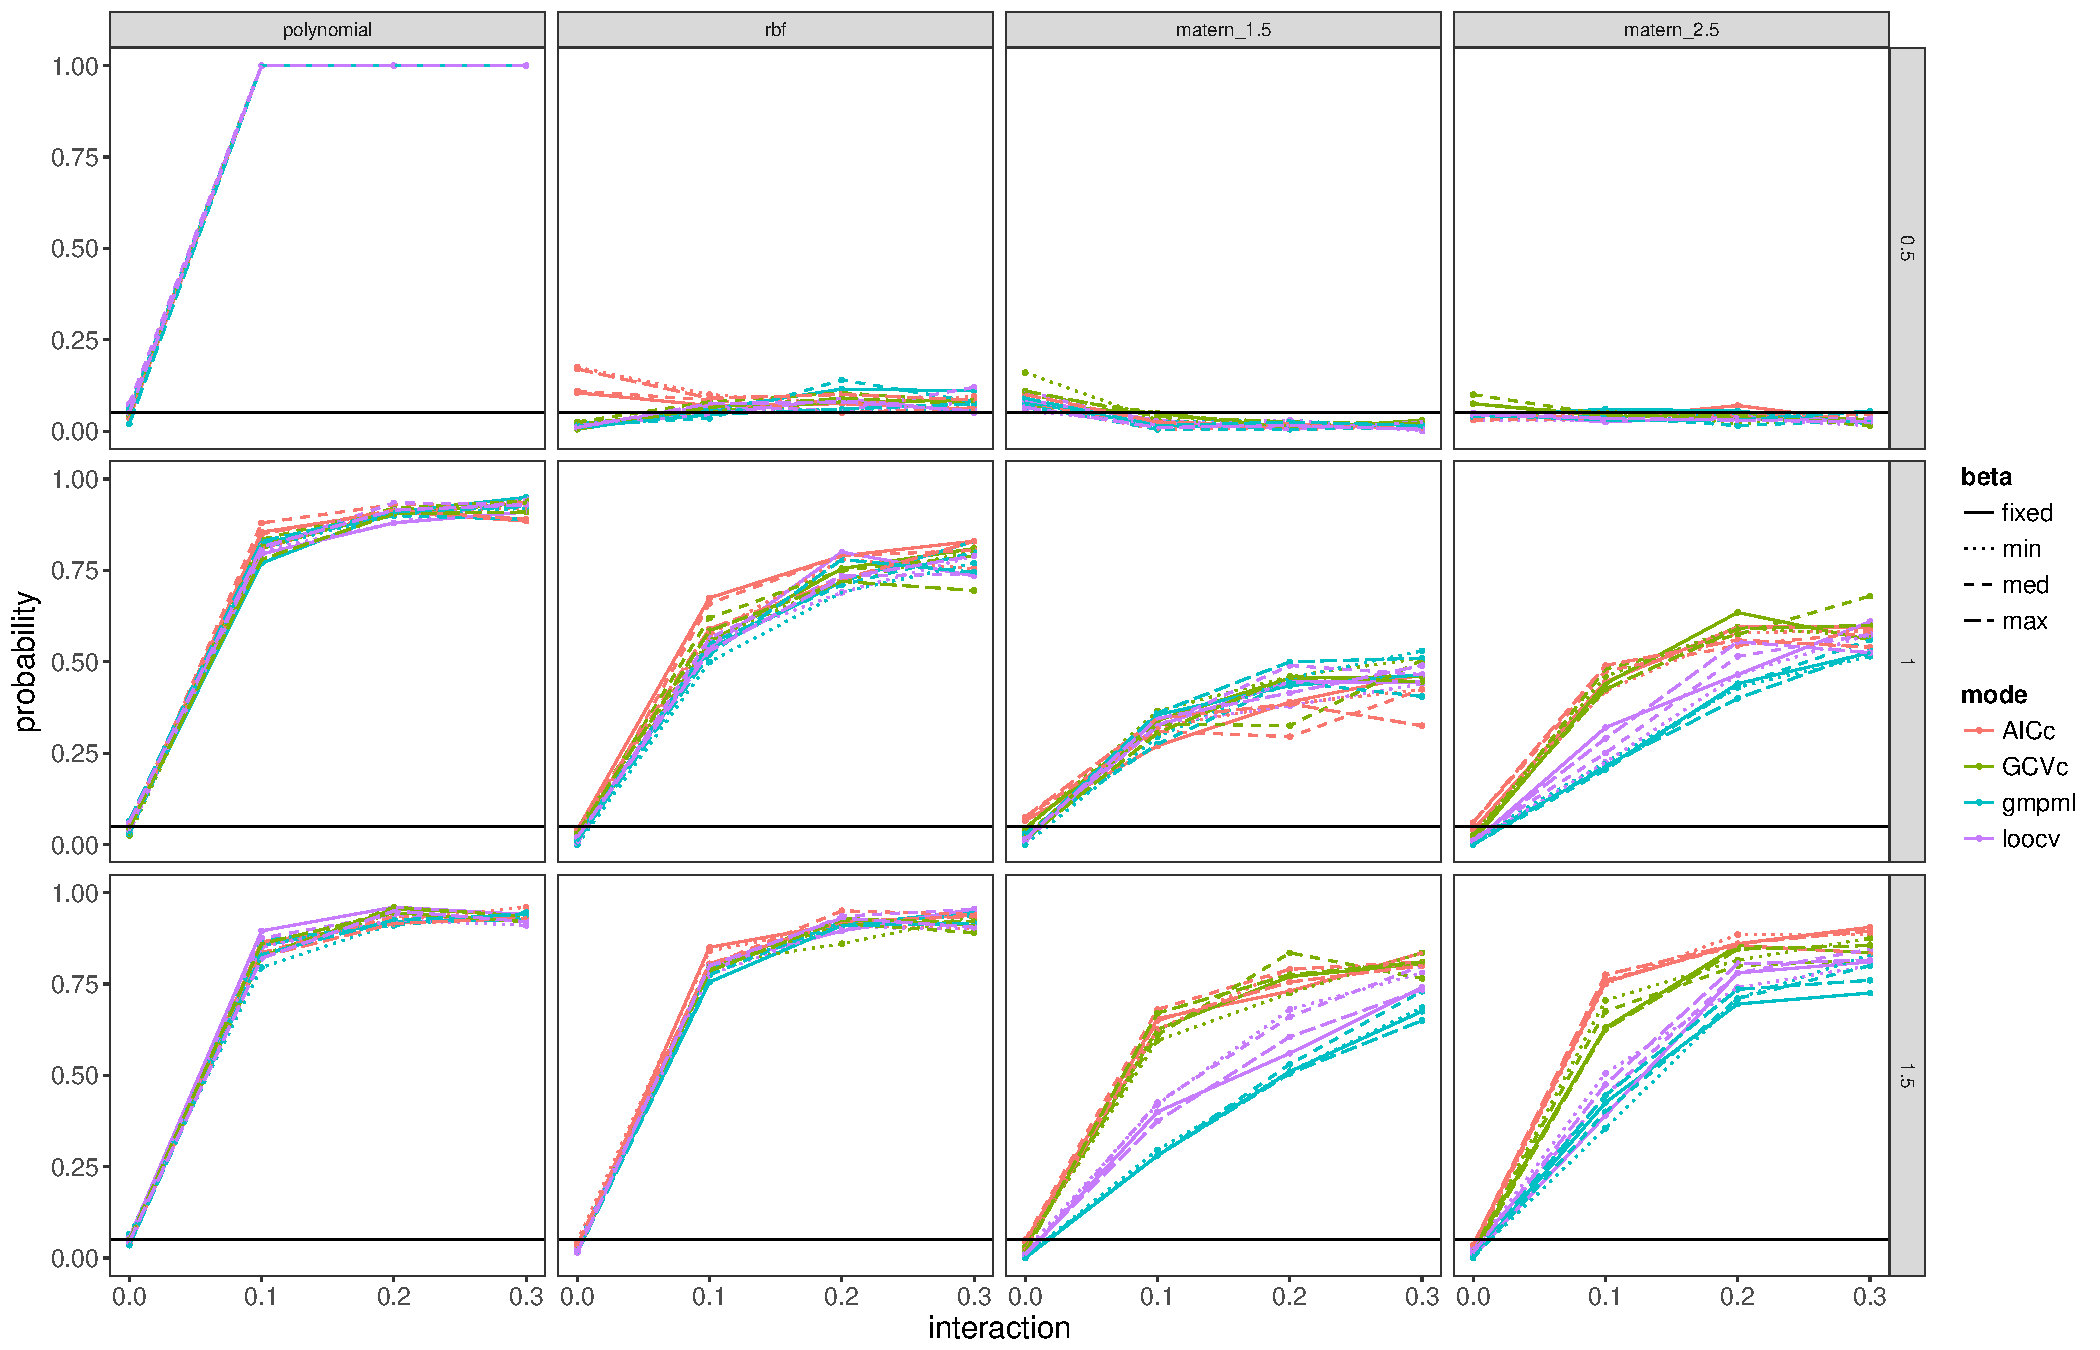
\includegraphics[width=0.9\columnwidth]{exp_A1} 
\caption{Asym, True kernel only}
\label{fig:res}
\end{center}
\end{figure}

\begin{figure}
\begin{center}
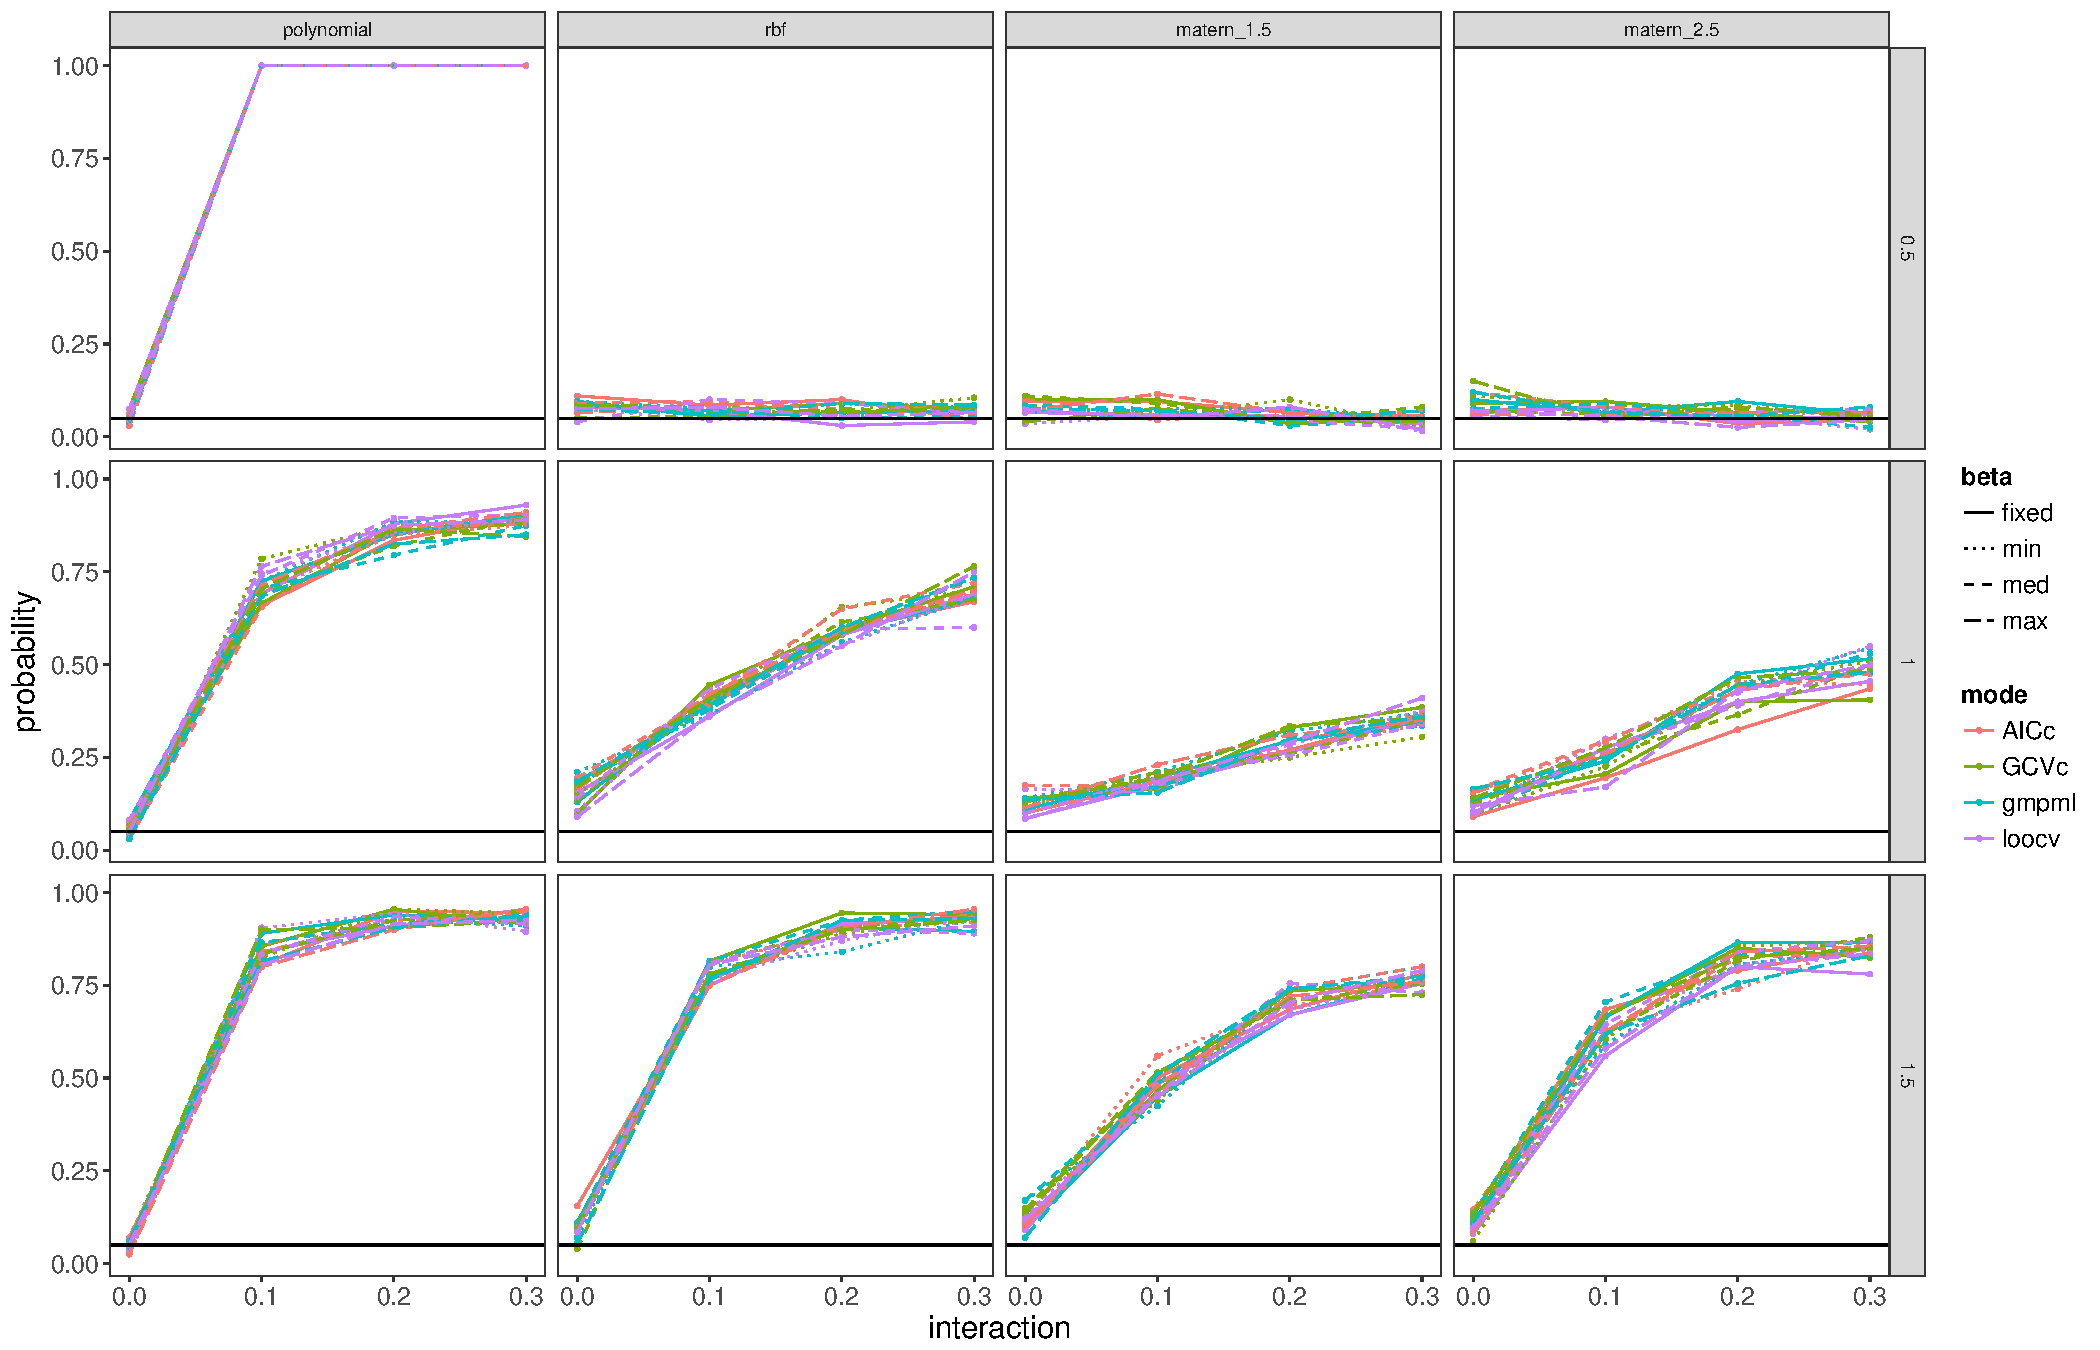
\includegraphics[width=0.9\columnwidth]{exp_A2} 
\caption{Asym, 3 Polynomial kernels}
\label{fig:res}
\end{center}
\end{figure}

\begin{figure}
\begin{center}
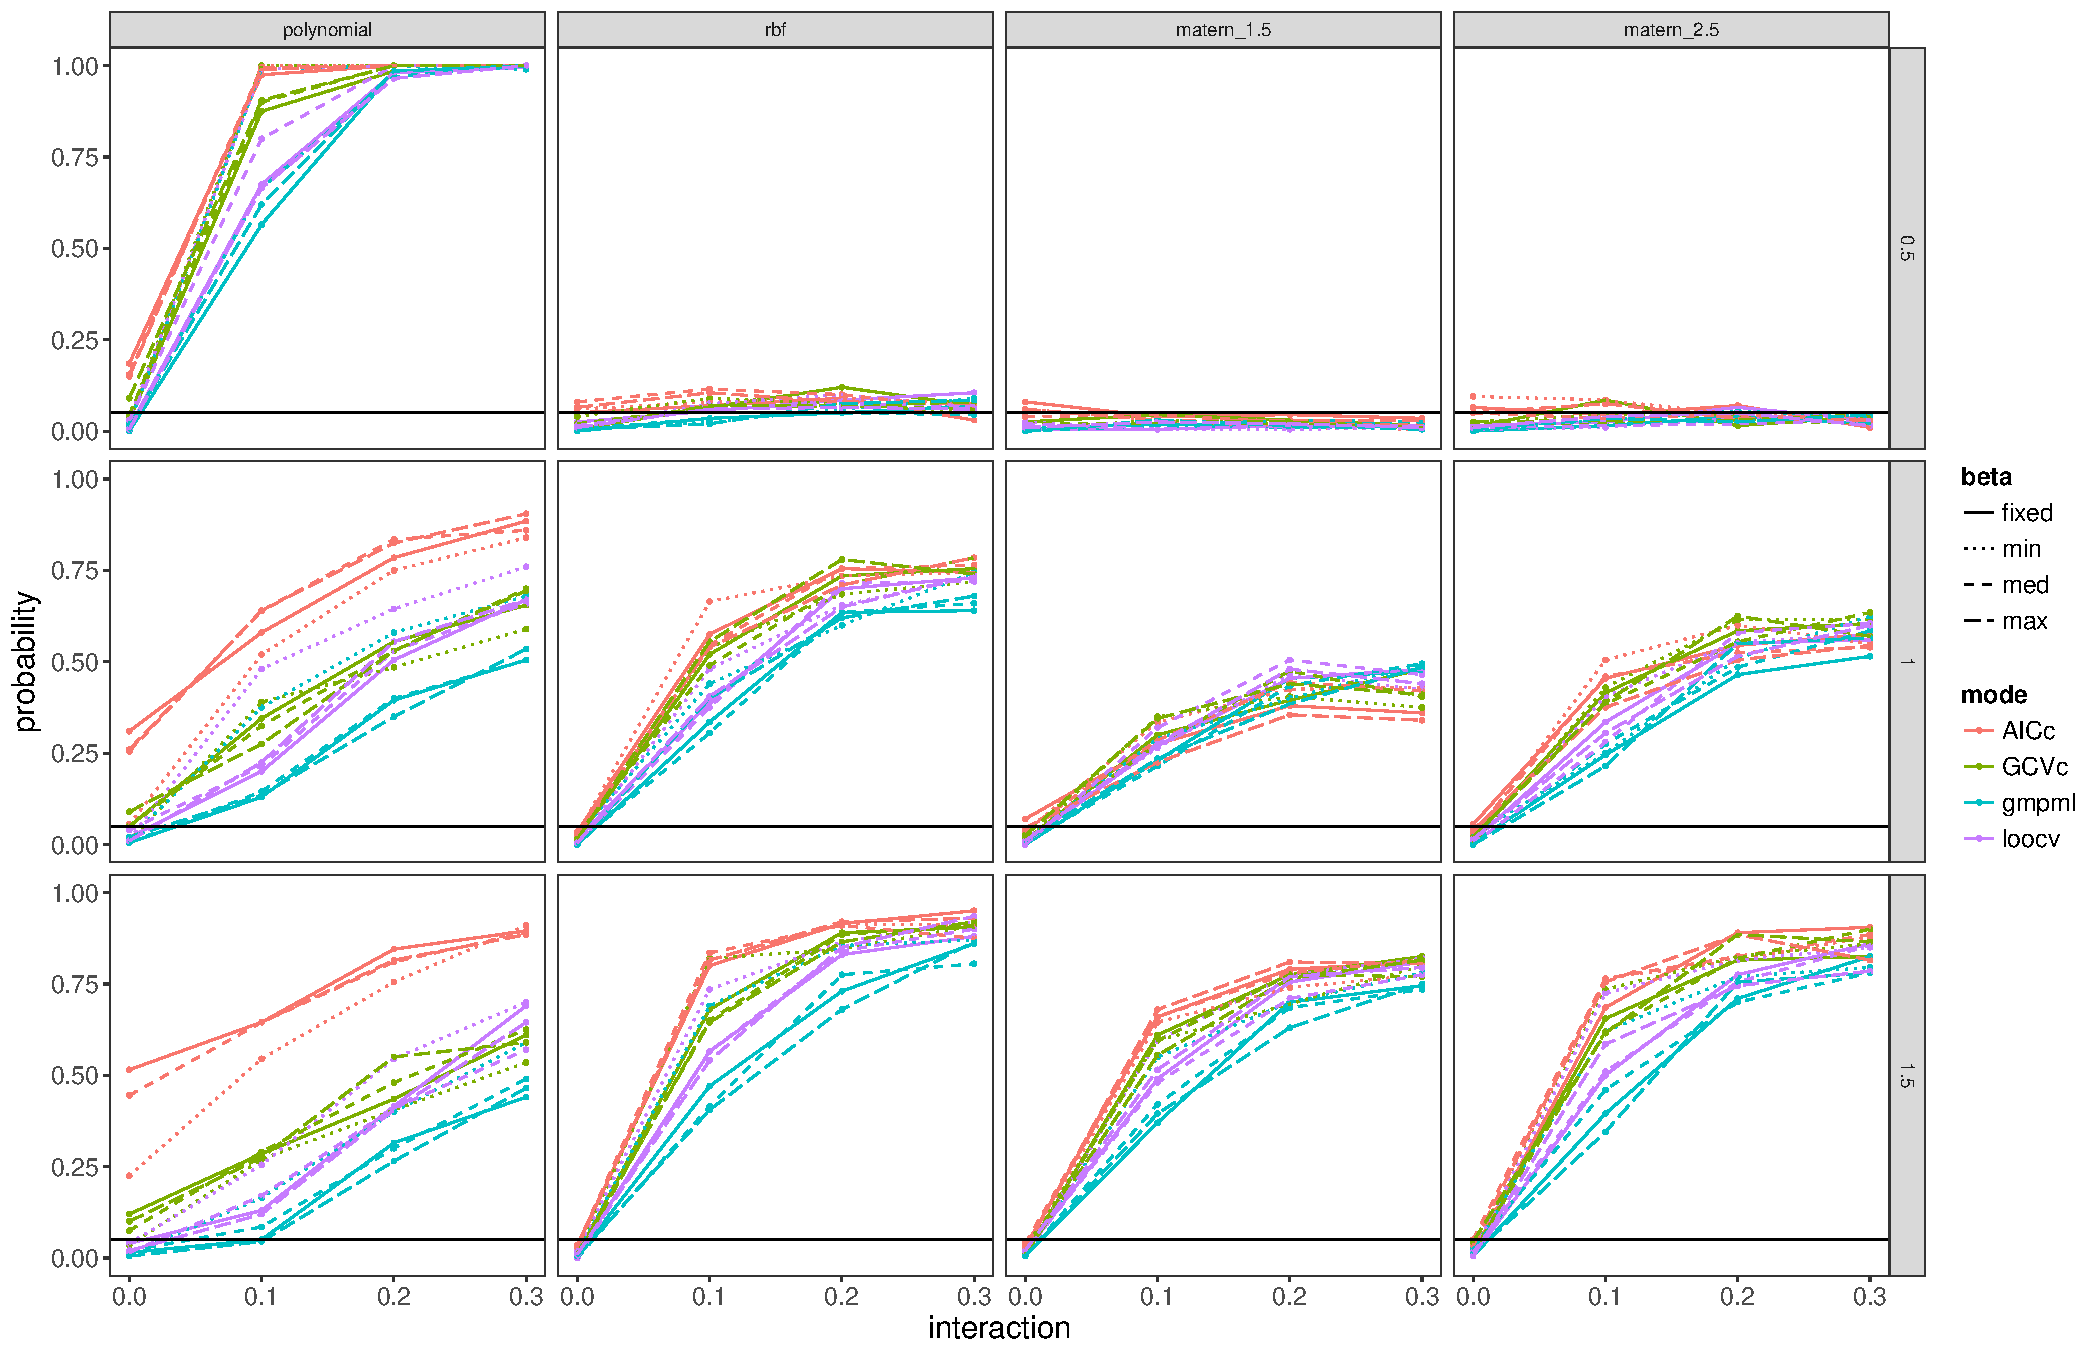
\includegraphics[width=0.9\columnwidth]{exp_A3} 
\caption{Asym, 3 RBF kernels}
\label{fig:res}
\end{center}
\end{figure}

\begin{figure}
\begin{center}
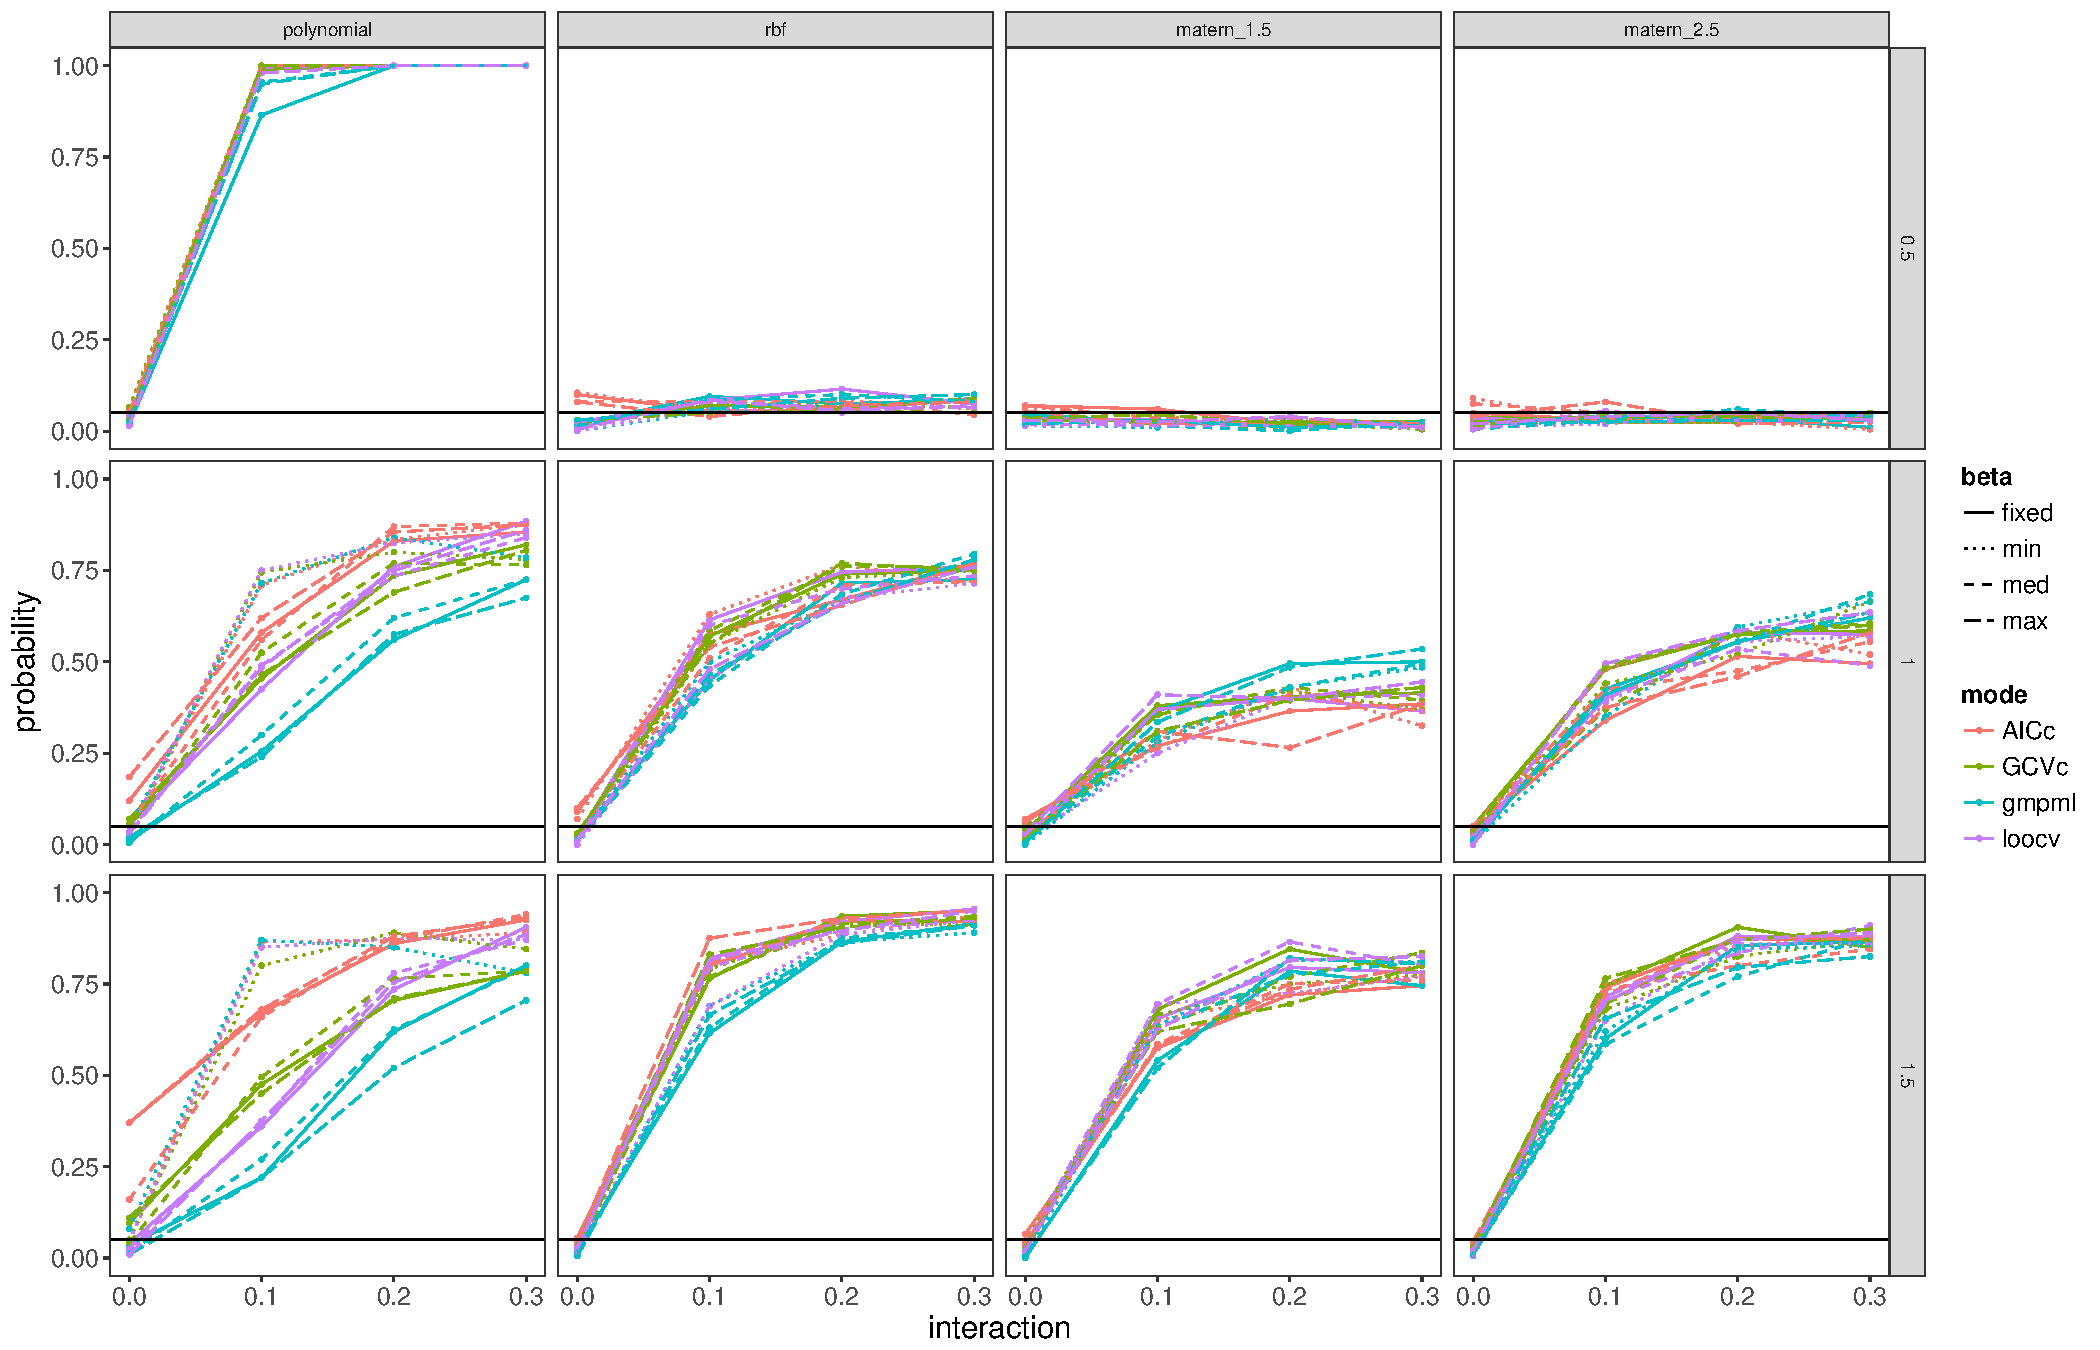
\includegraphics[width=0.9\columnwidth]{exp_A4} 
\caption{Asym, 3 Polynomial kernels and 3 RBF kernels}
\label{fig:res}
\end{center}
\end{figure}

\begin{figure}
\begin{center}
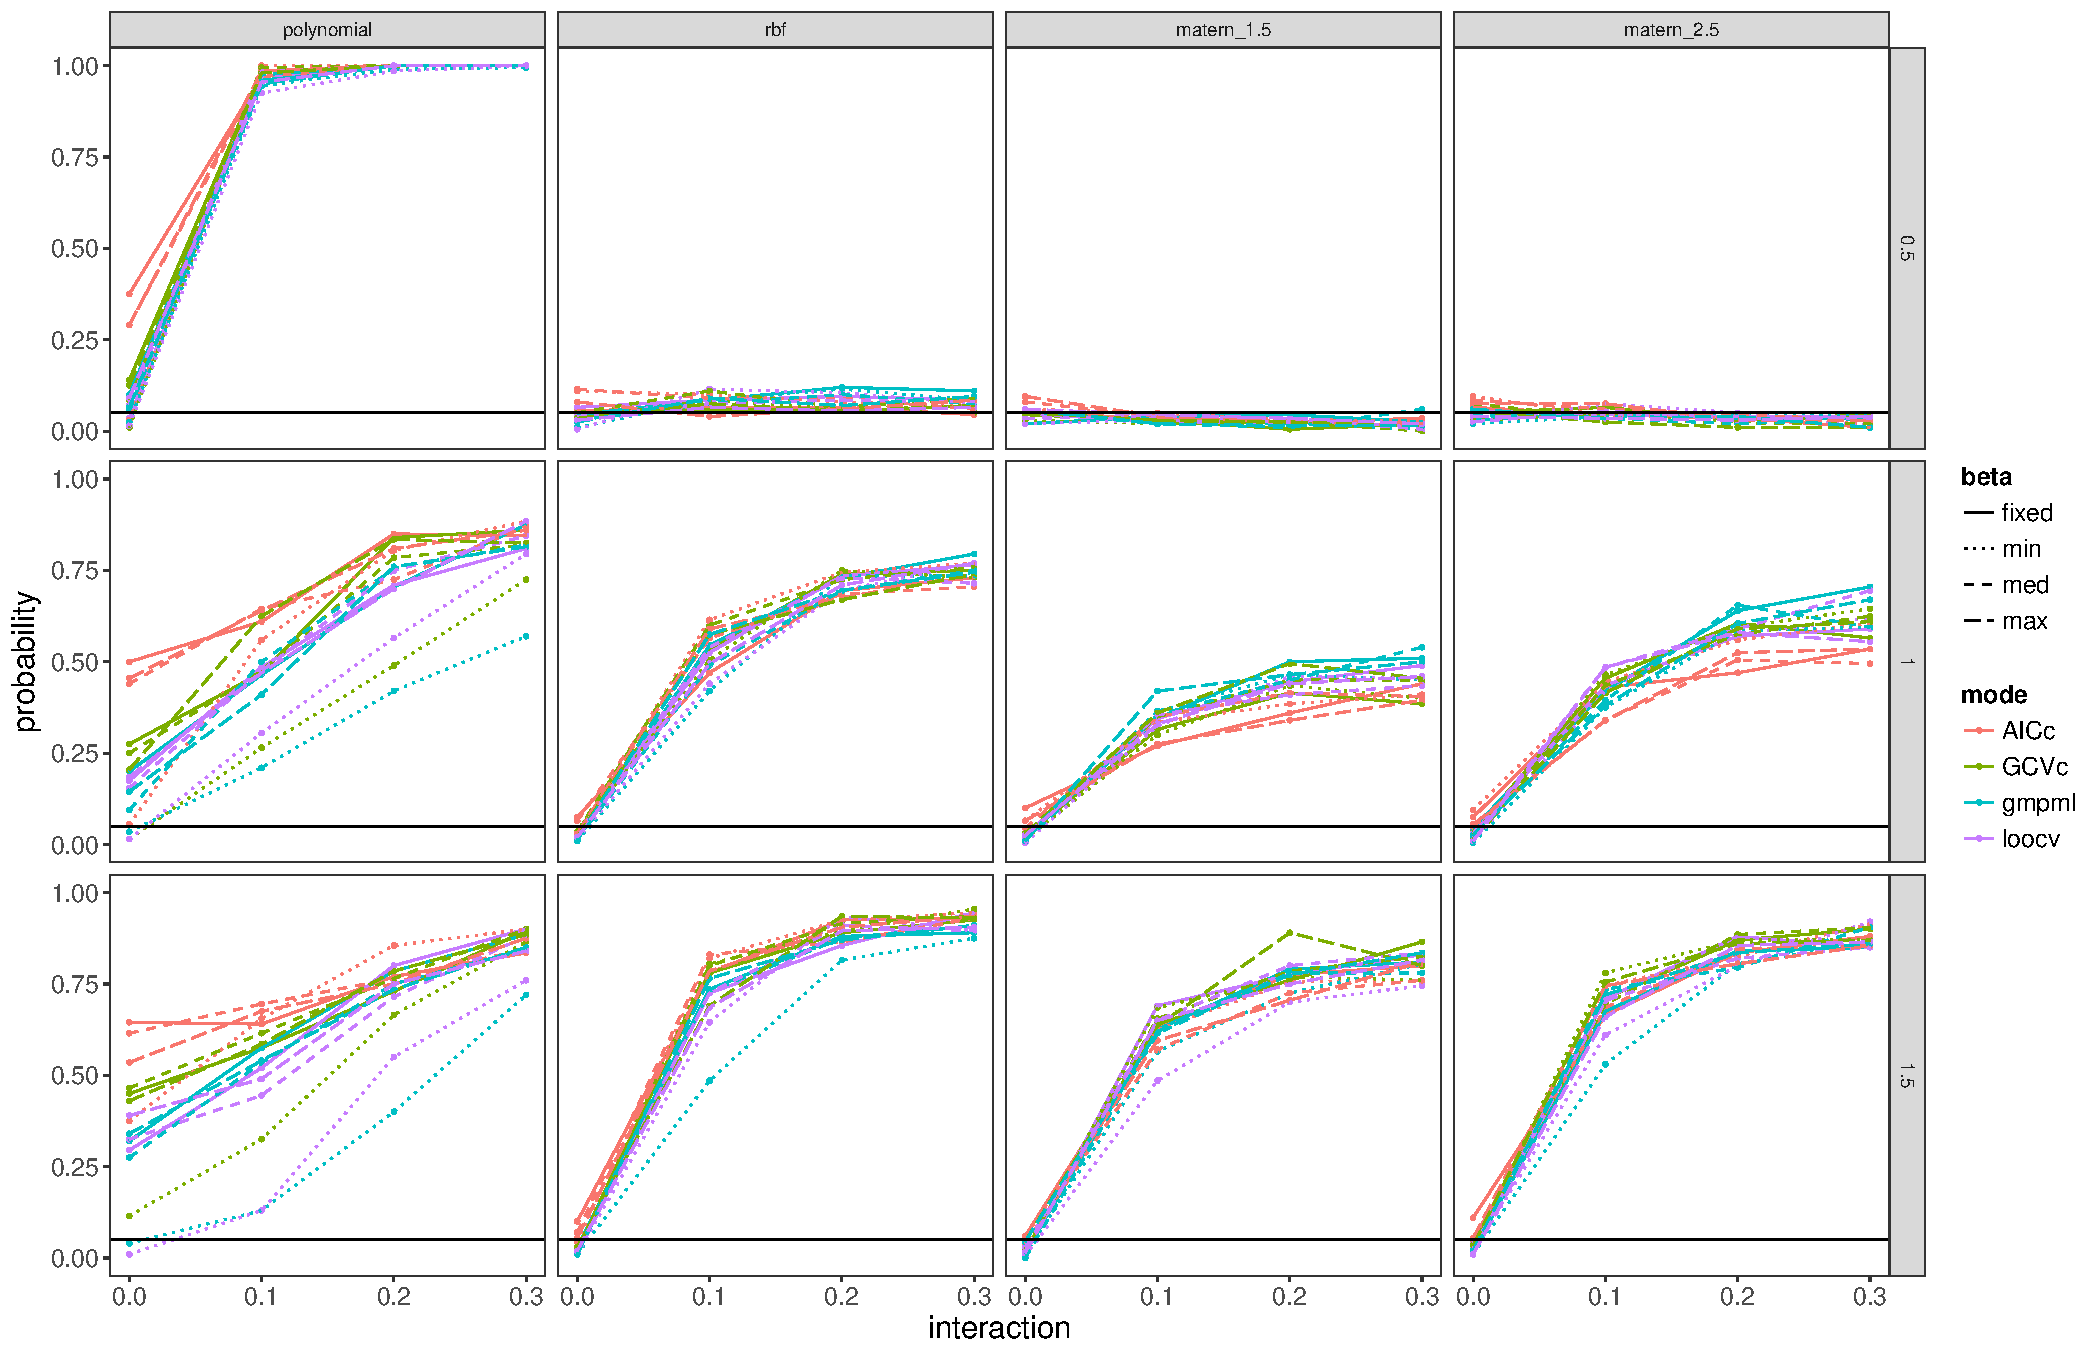
\includegraphics[width=0.9\columnwidth]{exp_A5} 
\caption{Asym, 3 Matern kernels and 3 RBF kernels}
\label{fig:res}
\end{center}
\end{figure}

\begin{figure}
\begin{center}
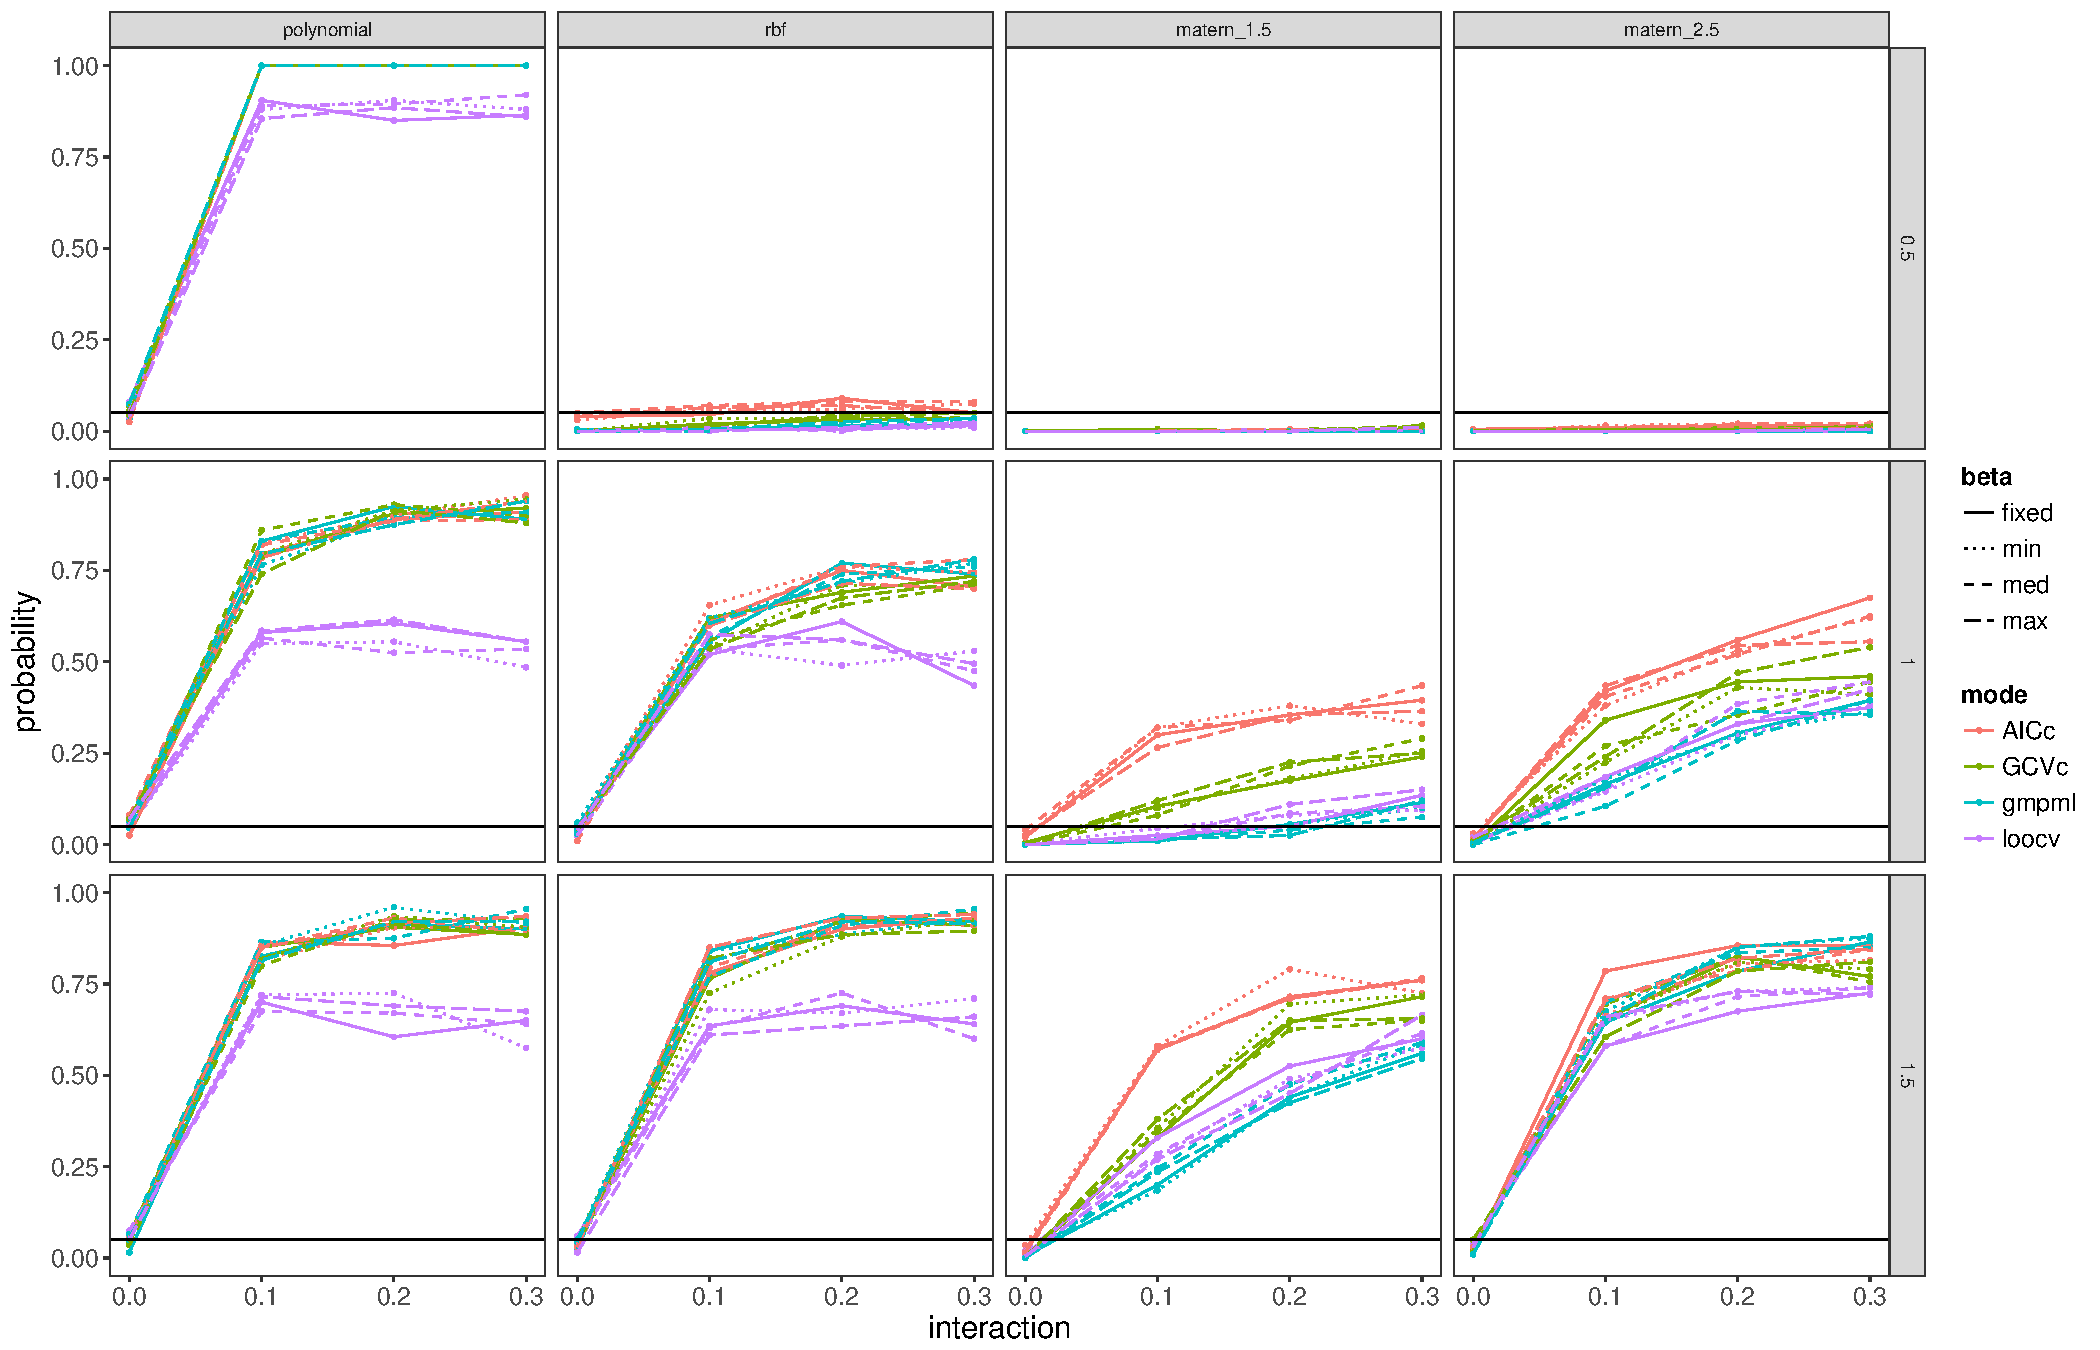
\includegraphics[width=0.9\columnwidth]{exp_B1} 
\caption{Boot, True kernel only}
\label{fig:res}
\end{center}
\end{figure}

\begin{figure}
\begin{center}
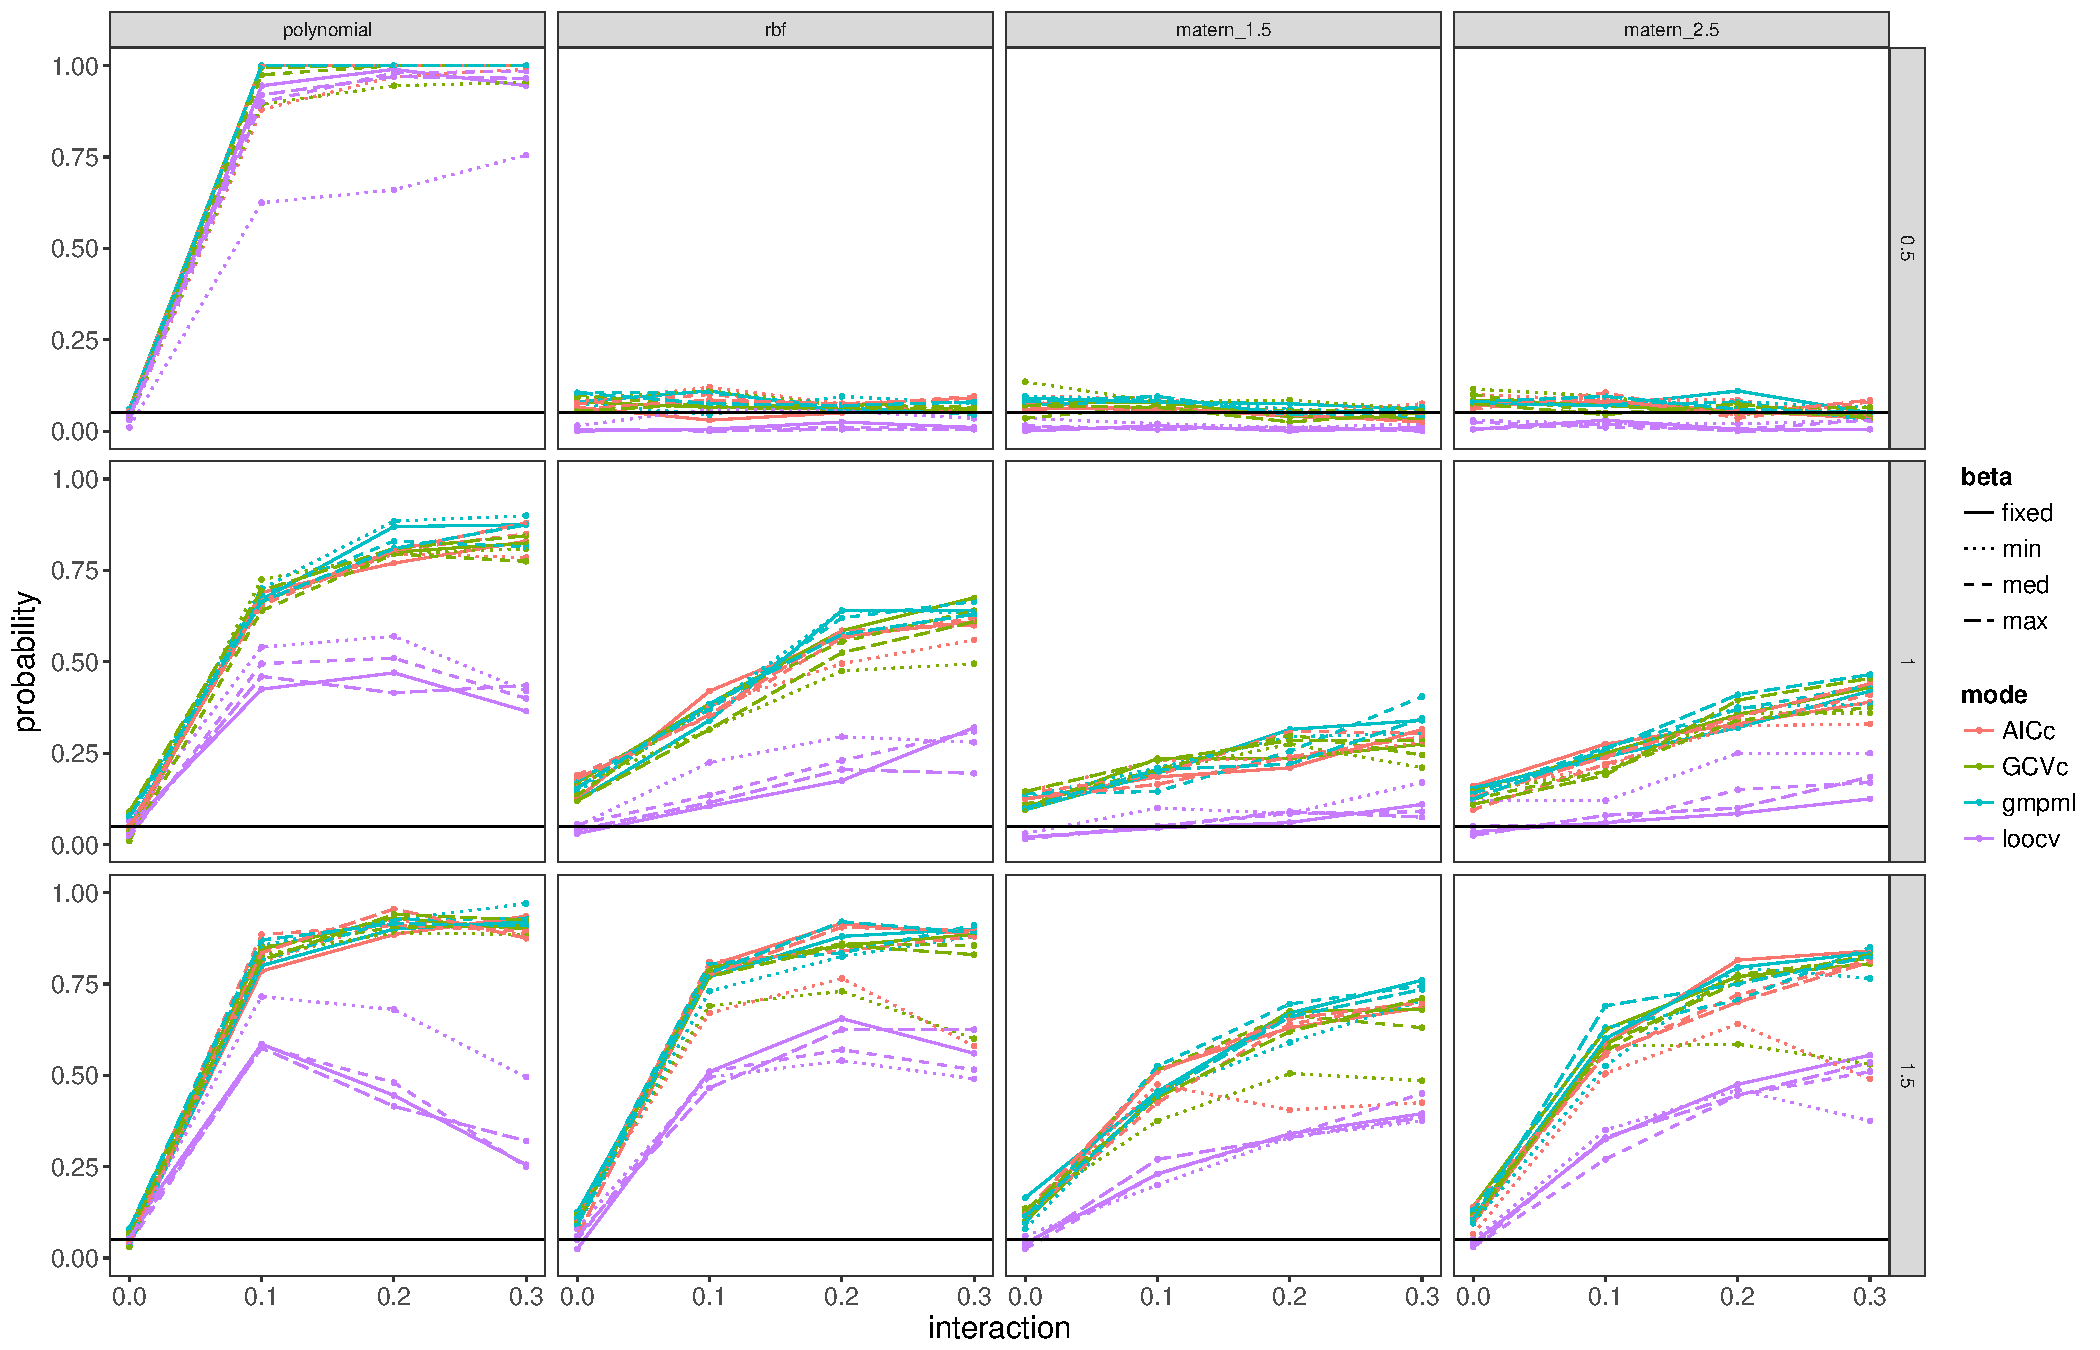
\includegraphics[width=0.9\columnwidth]{exp_B2} 
\caption{Boot, 3 Polynomial kernels}
\label{fig:res}
\end{center}
\end{figure}

\begin{figure}
\begin{center}
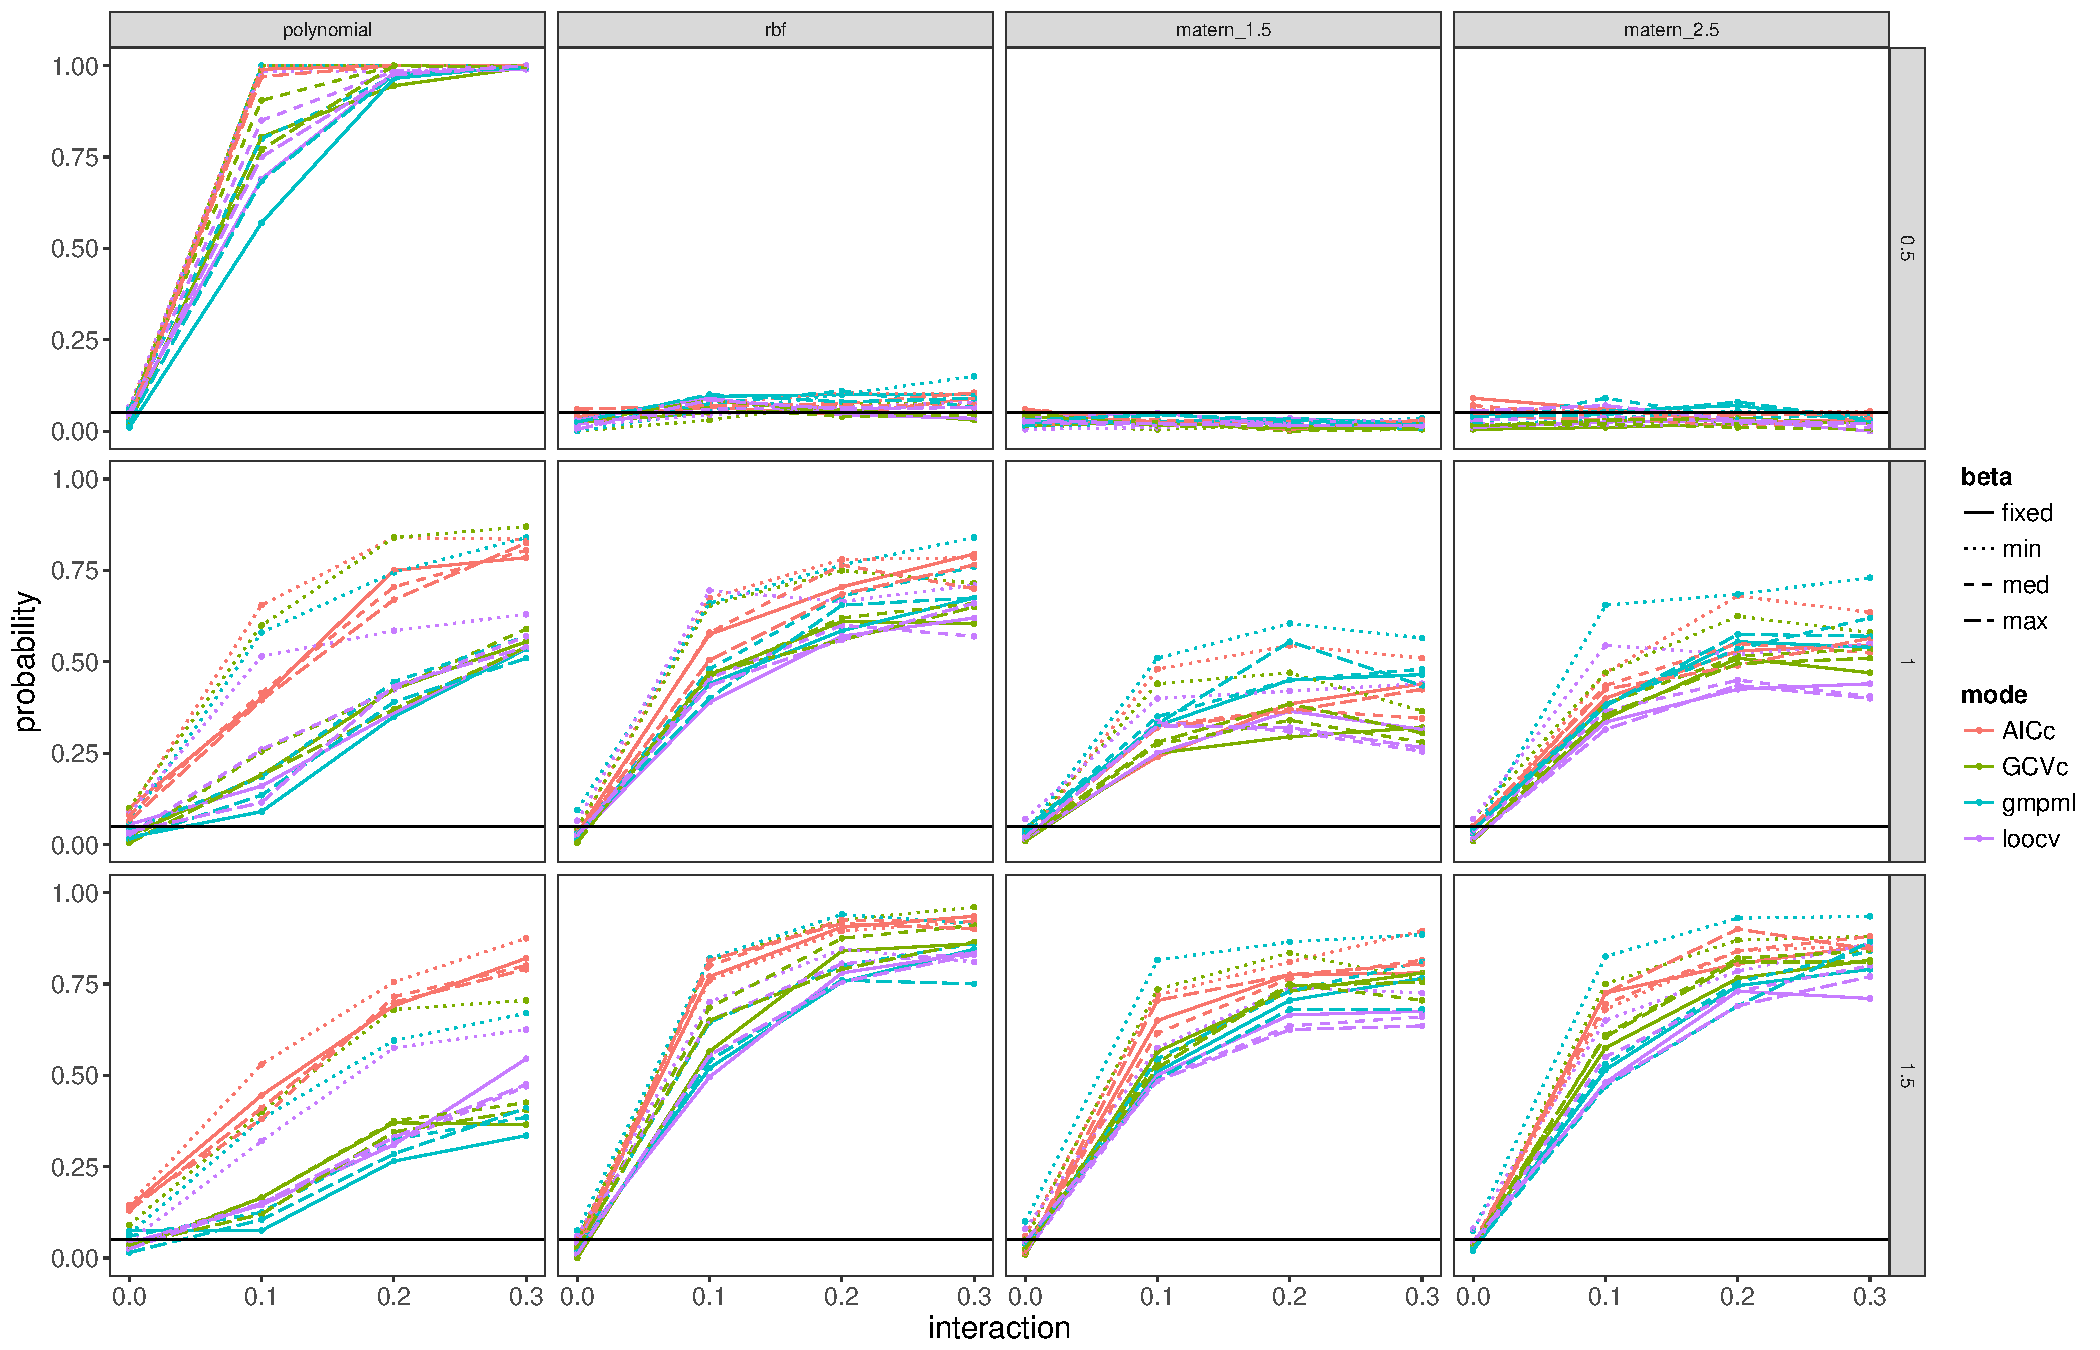
\includegraphics[width=0.9\columnwidth]{exp_B3} 
\caption{Boot, 3 RBF kernels}
\label{fig:res}
\end{center}
\end{figure}

\begin{figure}
\begin{center}
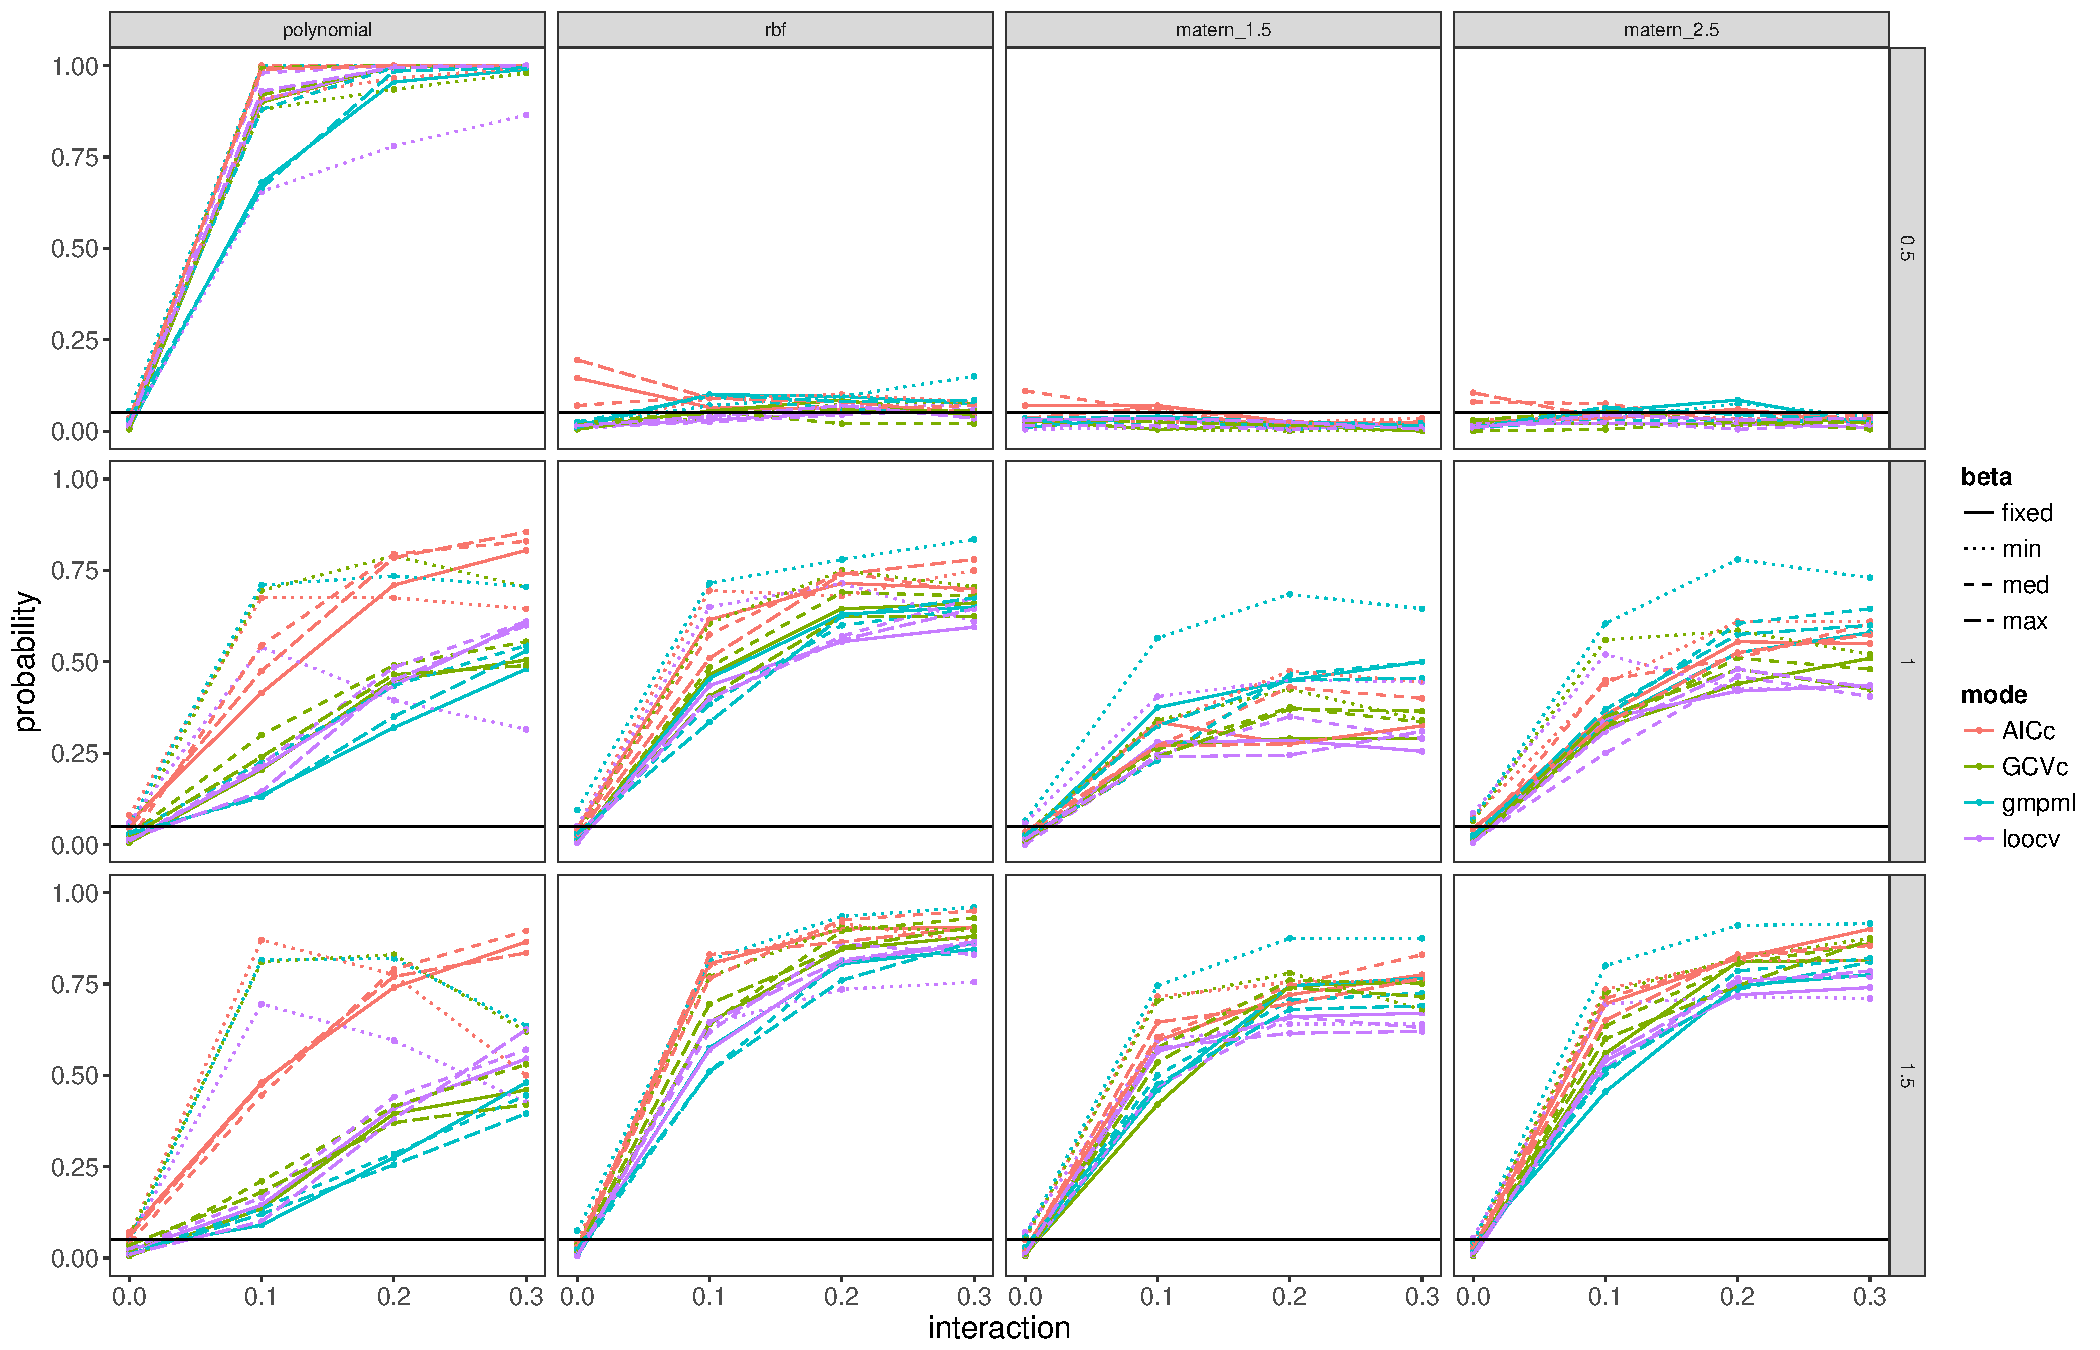
\includegraphics[width=0.9\columnwidth]{exp_B4} 
\caption{Boot, 3 Polynomial kernels and 3 RBF kernels}
\label{fig:res}
\end{center}
\end{figure}

\begin{figure}
\begin{center}
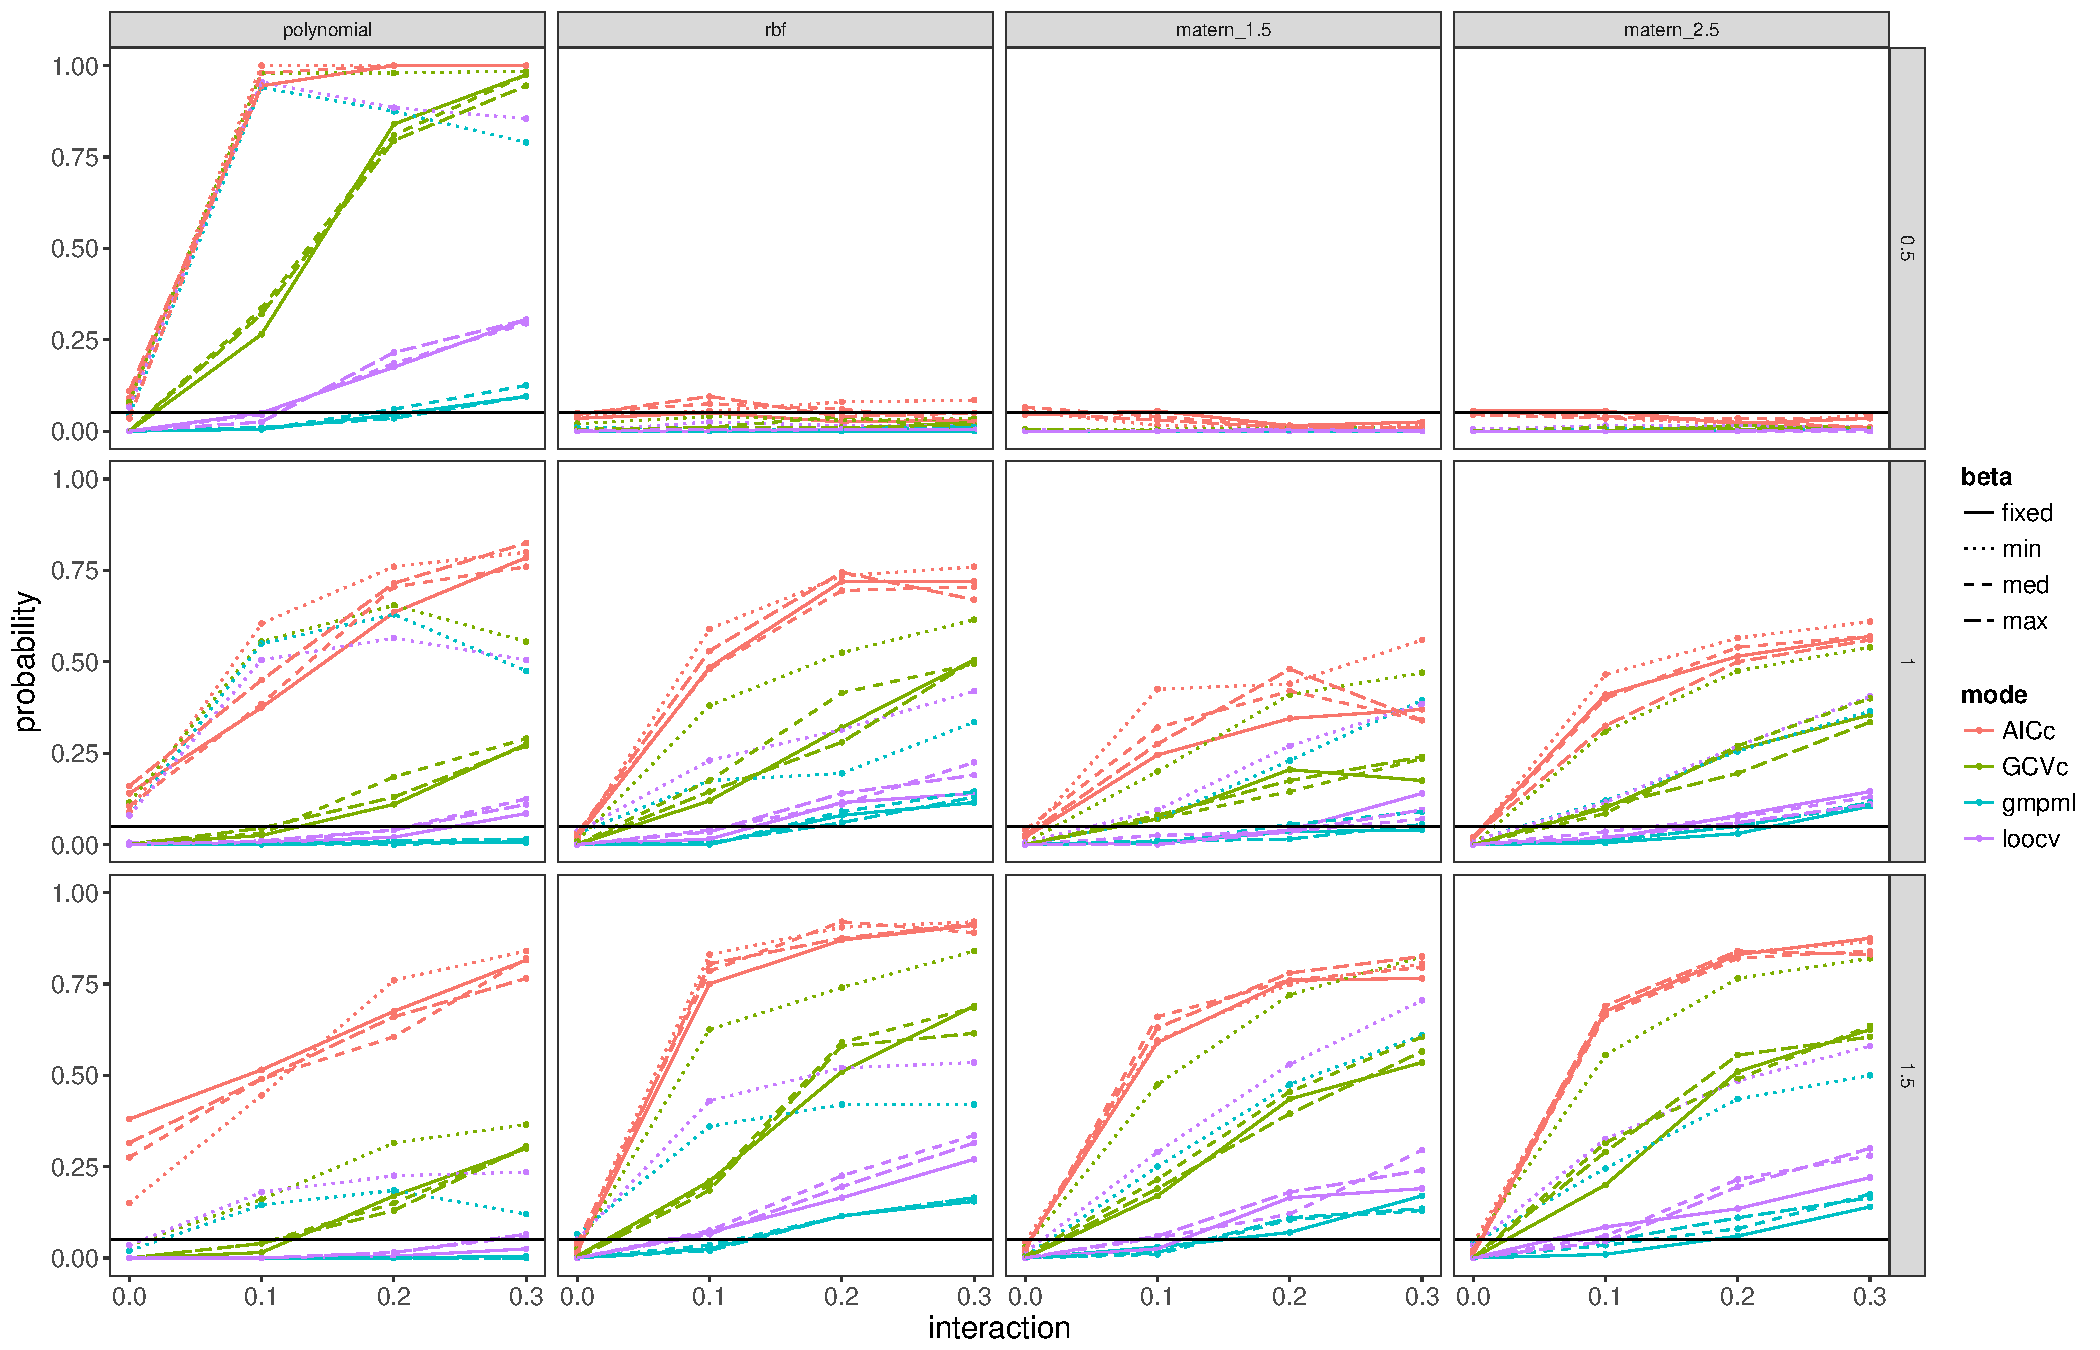
\includegraphics[width=0.9\columnwidth]{exp_B5} 
\caption{Boot, 3 Matern kernels and 3 RBF kernels}
\label{fig:res}
\end{center}
\end{figure}


\end{appendix}

%% -----------------------------------------------------------------------------


\end{document}
